\documentclass{itkmitlcoop}

\usepackage{afterpage}
\usepackage{graphicx,amsmath,latexsym,amssymb,amsthm}
\usepackage{indentfirst}
\usepackage{cite}
\graphicspath{ {images/} }
\usepackage{tabto}
\usepackage{tabularx}
\usepackage{ltablex}
\usepackage{longtable}
\usepackage[labelfont=bf]{caption}
\usepackage[labelfont=bf,tableposition=top]{caption}
\usepackage{float}
\captionsetup[table]{singlelinecheck=off}
\captionsetup[table]{labelsep=space}
\captionsetup[figure]{labelsep=space}

\makeindex
% ##### Set indent after new line on bibliography
\makeatletter
% \patchcmd{<cmd>}{<search>}{<replace>}{<succes>}{<failure>}
\patchcmd{\@chapter}{\addtocontents{lof}{\protect\addvspace{10\p@}}}{}{}{}% LoF
\patchcmd{\@chapter}{\addtocontents{lot}{\protect\addvspace{10\p@}}}{}{}{}% LoT
\makeatother
%1. Your thesis title (THAI)
\newcommand{\ThesisTiTle}{การพัฒนาชุดคำสั่งทดสอบอัตโนมัติ ด้วย แอพเพี่ยม บนฟลัตเตอร์ กรณีศึกษาของ โฮมโปร อีแคตตาล็อค แอปพลิเคชัน}
%2. Your thesis title (ENG)
\newcommand{\ThesisTiTleEng}{AUTOMATE TESTING WITH APPIUM ON FLUTTER WITH CASE STUDY BY HOMEPRO E-CATALOG APPLICATION}
%3. Your name
\newcommand{\AuName}{เสฎฐวุฒิ ไม้สนธิ์}
\newcommand{\AuNameEng}{Sedthawuth Maisonti}
%4. Your name ENG
\newcommand{\AuNameENG}{SEDTHAWUTH MAISONTI}
\newcommand{\AuNameENGSnakecase}{Sedthawuth Maisonti}
%5. Your student ID
\newcommand{\SId}{60070109}
%6. Your advisor
\newcommand{\Advisor}{ผศ.ดร.บุญประเสริฐ สุรักษ์รัตนสกุล}
\newcommand{\AdvisorEng}{Asst. Prof. Dr. Boonprasert Surakratanasakul}
%7. Your advisor employee
\newcommand{\Exami}{นางสาว อุบลรัตน์ พรหมสาขา ณ สกลนคร}
\newcommand{\ExamiEng}{ test }
%8. สถานประกอบการ
\newcommand{\Company}{บริษัท โฮมโปรดักส์ เซ็นเตอร์ จำกัด (มหาชน)}
%9. ภาคเรียนที่ (in normal letters)
\newcommand{\Sem}{1}
%10. ปีการศึกษา (in normal letters)
\newcommand{\AcaY}{2563}
%11. ปีการศึกษา (in normal letters)
\newcommand{\AcaYAD}{2020}
%12. วันส่งรายงาน
\newcommand{\SubD}{23 พฤศจิกายน พ.ศ. 2563}
%13. วันเริ่มทำงาน
\newcommand{\StartDWork}{1 มิถุนายน พ.ศ. 2563}
%14. วันสุดท้ายของการทำงาน
\newcommand{\EndDWork}{30 พฤศจิกายน พ.ศ. 2563}
%15. ที่อยู่สถานประกอบการ
\newcommand{\Address}{96/27 หมู่ที่ 9 ต.บางเขน อ.เมือง จ.นนทบุรี 11000}
%16. เว็บไซต์สถานประกอบการ
\newcommand{\Website}{www.homepro.co.th}
%17. ตำแหน่งานที่ปฏิบัติ
\newcommand{\Position}{PROGRAMMER}

\newcommand{\Department}{เทคโนโลยีสารสนเทศ}
\newcommand{\DepartmentEng}{Information Technology}

\newcommand{\Branch}{เทคโนโลยีสารสนเทศ}

\begin{document}    
    \pagestyle{empty}
    \frontmatter

    \makecover    
    \makeinnercover
    \makeinnercovereng
    \makecopyright
    \makeletter
    \makeack{
        \begin{enumerate}
            \item นางสาว อุบลรัตน์ พรหมสาขา ณ สกลนคร \quad ตำแหน่ง ผู้จัดการทั่วไป-สายบริการส่งเสริมการขาย (พนักงานที่ปรึกษา)
        \end{enumerate}
    }
    \makeapproveletter
   
    % Setting margin for page numbering on frontmatter
    \newgeometry{top=1in, bottom=1in, left=1.5in, right=1in, includefoot}

    \makeabstract{
        รายงานเล่มนี้จะนำเสนอผลลัพธ์ และขั้นตอนการดำเนินงานเพื่อให้ได้ชุดคำสั่งทดสอบอัตโนมัติที่ไว้ใช้
        ทดสอบกับแอปพลิเคชัน โฮมโปร อีแคตตาล็อค ที่ใช้กับระบบปฎิบัติการ Android ซึ่งนักศึกษาได้ปฎิบัติสหกิจศึกษา ณ {\Company}
        ตำแหน่ง Programmer

        {\Company} ได้ทำการพัฒนาแอปพลิเคชันออกมาหลายตัวหนึ่งในนั้นคือ แอปพลิเคชัน โฮมโปร อีแคตตาล็อค ที่ถูกพัฒนาขึ้นมาด้วย
        Flutter เมื่อจะนำขึ้นมาใช้งานจริงจะต้องทำการทดสอบก่อนเสมอทำให้ต้องนั่งทดสอบแบบ Manual ทำให้ใช้เวลานาน

        ทาง {\Company} จึงอยากทดสอบการนำ การพัฒนาชุดคำสั่งทดสอบอัตโนมัติมาใช้เพื่อลดเวลาในการทดสอบมาใช้ว่าจริงหรือไม่
        และดีกับการนำมาประยุกต์ใช้หรือไม่อีกทั้งต้องการนำชุดคำสั่งทดสอบอัตโนมัติขี้นไปทดสอบบน AWS Device Farm เพื่อทดสอบอุปกรณ์ได้หลากหลายมากขึ้

    }
    \pagestyle{fancy}
	\pagenumbering{Roman}
   \makeabstracteng{
       This report will offer result and development process to build automate test script for application HomePro E-Catalog. That run on android OS
       which cooperative education student work in Home Product Center Public Company Limited as Programmer.

       Home Product Center Public Company Limited create a lot of application which one of that is HomePro E-Catalog that are made with Flutter Framework.
       Before application go to production. The application need to be tested manual which take a longtime.

       So Home Product Center Public Company Limited want to try bring automate testing to help reduce time cost and see if it also worth to use it
       in other project and they also want to run automate test on AWS Device Farm for various devices.
   }

    \newpage
    \addcontentsline{toc}{chapter}{สารบัญ}
    \tableofcontents
    
    \newpage
    \addcontentsline{toc}{chapter}{สารบัญตาราง}
    \listoftables    
    
    \newpage
    \addcontentsline{toc}{chapter}{สารบัญรูป}
    \listoffigures
    
    % Reset frontmatter page numbering margin, back to original margin from class file
    \restoregeometry

    \mainmatter
    \pagestyle{plain}
    \pagenumbering{arabic}
    \chapter{บทนำ}
\thispagestyle{empty}
\label{chapter:introduction}

\section{ที่มาและความสำคัญ}
    {\Company} เป็นบริษัทขายปลีกที่จำหน่ายสินค้าและให้บริการที่เกี่ยวข้องกับการก่อสร้าง ตกแต่ง ต่อเติม ซ่อมแซม ปรับปรุง อาคาร บ้าน และที่อยู่อาศัยแบบครบวงจร
    แต่หากว่า โฮมโปรหน้าร้านบางสาขาอาจจะไม่มีสินค้าที่ลูกค้าต้องการอยู่เพราะขนาดของสาขาของโฮมโปรมีหลายขนาดตั้งแต่ร้านขนาดเล็กที่ตั้งอยู่ในห้างสรรพสินค้าของเจ้าอื่น
    ไปจนถึงตั้งแยกออกมาเป็นห้างสรรพสินค้าขนาดใหญ่ของตนเองจึงทำให้สินค้าที่มีอยู่ไม่สามารถแสดงได้ทั้งหมดตามขนาดโฮมโปรจึงจัดทำแอปพลิเคชัน E-Catalog ขึ้นมา
    แอปพลิเคชัน E-Catalog คือแอปพลิเคชันในการสนับสนุนการขายของพนักงานสาขาในการที่จะแสดงสินค้าที่โฮมโปรมีแต่สาขาที่ลูกค้าอยู่ไม่มีได้ยกตัวอย่างเช่น โฮมโปร
    สาขา ประชาชื่น ไม่มีแอร์รุ่นที่ลูกค้าต้องการพนักงานขายของสาขาสามารถแสดงรูปตัวอย่างสินค้าและคุณสมบัติของสินค้าผ่านแอปพลิเคชันให้ลูกค้าดูว่าตรงกับความต้องการลูกค้าหรือไม่และแสดง
    ถึงสาขาที่มี แอร์อยู่ได้อีกทั้งยังสามารถสั่งจองสินค้านั้นจากสาขาที่มีผ่านทางแอปพลิเคชันได้เลยเพียงแค่กรอกเบอร์โทรศัพท์ และ แอปพลิเคชันสามารถใช้ในการช่วยขายสินค้าที่เกี่ยวข้องกัน
    ให้กับลูกค้าเพิ่มเติมได้ เช่น ลูกค้าเลือกซื้อประตูพนักงานสาขาสามารถแสดงลูกบิดที่ดูเหมาะสมเข้ากับประตูนั้นได้ เป็นต้น
    เพื่อป้องกันข้อผิดพลาดก่อนนำแอปพลิเคชันไปใช้จริงต้องทดสอบเพื่อสังเกตหาข้อผิดพลาดทุกครั้งโดยแต่ละครั้งหากตัวแอปพลิเคชันเกิดการแก้ไขแม้ว่าจะมากหรือน้อยก็ตาม
    เพราะการแก้ไขแต่ละครั้งอาจจะส่งผลกระทบกับส่วนอื่นๆของแอปพลิเคชันได้ แต่จะเสียแรงงานและเวลากับการทดสอบได้หากเกิดการแก้ไขบ่อยครั้ง
    ดังนั้นบริษัท โฮมโปรดักส์ เซ็นเตอร์ จํากัด (มหาชน) จึงได้เล็งเห็นถึงความสําคัญของการทดสอบ
    แอปพลิเคชันแบบอัตโนมัติ จึงให้นักศึกษาปฏิบัติงานโครงการทวิภาคีสถาบันเทคโนโลยีพระจอมเกล้าเจ้าคุณทหารลาดกระบัง นาย เสฎฐวุฒิ ไม้สนธิ์ ทำการทดสอบโดยการเขียนชุดคำสั่งทดสอบอัตโนมัติ (automate testing) ให้ใช้คู่กับ AWS Device Farm
    ในการพัฒนาชุดคำสั่งทดสอบอัตโนมัติเพื่อลดระยะเวลาและแรงงานในการทดสอบแอปพลิเคชันแบบเดิม

\section{วัตถุประสงค์}
    \begin{enumerate}
        \item เพื่อพัฒนาทักษะของตนเองในการพัฒนาชุดคำสั่งทดสอบอัตโนมัติ
        \item เพื่อลดข้อผิดพลาดจากการทดสอบแอปพลิเคชันแบบ Manual
        \item ลดเวลาการทดสอบและส่งมอบแอปพลิเคชันได้รวดเร็วขึ้น
        \item เพื่อเป็นต้นแบบในการทดสอบแอปพลิเคชันตัวอื่นของบริษัทต่อไป
    \end{enumerate}

\section{ประวัติ และรายละเอียดสถานประกอบการ}
    \subsection{ชื่อ และสถานที่ตั้งของสถานประกอบการ}
        {\Company}

        ที่อยู่ {\Company} สำนักงานใหญ่

        {\Address}
    \subsection{ประวัติความเป็นมาของสถานประกอบการ}
        บมจ. โฮม โปรดักส์ เซ็นเตอร์ จดทะเบียนจัดตั้งขึ้นเมื่อวันที่ 27 มิถุนายน 2538 โดยเป็นการร่วมลงทุนของ บมจ. แลนด์แอนด์เฮ้าส์ และ บมจ. ควอลิตี้เฮ้าส์ บริษัทฯ เริ่มต้นเปิดดำเนินการที่สาขารังสิตในเดือนกันยายน 2539 เป็นแห่งแรก โดยใช้ชื่อทางการค้าว่า “โฮมโปร” (HomePro)
        บริษัทฯ ได้จดทะเบียนแปรสภาพเป็นบริษัทมหาชนในวันที่ 29 พฤษภาคม 2544 ด้วยทุนจดทะเบียนเริ่มต้น 150 ล้านบาท ต่อมาได้จดทะเบียนเป็นบริษัทรับอนุญาตในตลาดหลักทรัพย์แห่งประเทศไทยในวันที่ 30 ตุลาคม 2544 โดยใช้ชื่อย่อหลักทรัพย์ว่า “HMPRO”
        ในวันที่ 26 พฤษภาคม 2548 บริษัทฯ ได้จดทะเบียนจัดตั้งบริษัท มาร์เก็ต วิลเลจ จำกัด โดยมีวัตถุประสงค์เพื่อบริหารพื้นที่ให้เช่า พร้อมกับให้บริการทางด้านสาธารณูปโภค เริ่มต้นดำเนินการในไตรมาสแรก ปี 2549 ที่โครงการ “หัวหิน มาร์เก็ต วิลเลจ” (Hua-Hin Market Village)
        และในปี 2549 บริษัทฯ ได้ถูกคัดเลือกให้เป็นหลักทรัพย์ในกลุ่ม SET100
        ในปี 2553 บริษัทฯ ได้รับคัดเลือกให้เป็นหลักทรัพย์ในกลุ่ม SET 50  และได้เปิดดำเนินการครบ 15 ปี มีสาขาทั้งสิ้น 40 แห่ง เป็นสาขาในเขตกรุงเทพฯ และปริมณฑล 19 แห่ง ในต่างจังหวัด 21 แห่ง
        \begin{figure}[H]
            \centering
            
\includegraphics[width=0.5\textwidth]{homepro-logo}
            \caption{ตราตราสัญลักษณ์ บริษัท โฮมโปรดักส์ เซ็นเตอร์ จำกัด (มหาชน)}\label{homepro-logo}
        \end{figure}

    \subsection{ลักษณะการประกอบการ ผลิตภัณฑ์/ผลิตผล}
    \begin{enumerate}
        \item ธุรกิจค้าปลีก
        \begin{itemize}
            \item[-] สินค้าที่เกี่ยวกับวัสดุก่อสร้าง สี อุปกรณ์ ปรับปรุงบ้าน ห้องน้ำและสุขภัณฑ์ เครื่องครัว อุปกรณ์ และ เครื่องใช้ไฟฟ้า
            \item[-] สินค้าประเภทเครื่องนอน พรม ผ้าม่าน เฟอร์นิเจอร์ โคมไฟ สินค้าตกแต่ง และอุปกรณ์เครื่องใช้ ภายในบ้าน  
        \end{itemize}
        \item  บริการที่เกี่ยวเนื่องกับธุรกิจค้าปลีก เนื่องจากสินค้าส่วนใหญ่ของบริษัทฯ เป็นสินค้าที่มี รายละเอียดของวิธีการ และขั้นตอนการใช้งานที่ต้องมีการ ถ่ายทอดให้กับลูกค้า บริษัทฯ จึงจัดให้มีบริการด้านต่างๆ ที่เกี่ยวข้อง โดยเริ่มตั้งแต่การให้คำ ปรึกษา และข้อมูลที่จะ เป็นประโยชน์ต่อการตัดสินใจเพื่อให้ลูกค้าสามารถเลือก ซื้อสินค้าได้ตรงกับวัตถุประสงค์การใช้งานมากที่สุด อีกทั้ง ยังมีบริการ “โฮม เซอร์วิส” (Home Service) ที่ให้บริการ ครอบคลุมงานออกแบบห้องด้วยระบบคอมพิวเตอร์ 3 มิติ (3D Design) และงานบริการดังต่อไปนี้
        \begin{itemize}
            \item[-] งานติดตั้ง ย้ายจุด แก้ปัญหา (Installation Service)
            \item[-] งานตรวจเช็ค ทำความสะอาด/บำรุงรักษาเครื่องใช้ ไฟฟ้าต่างๆ (Maintenance Service)
            \item[-] งานปรับปรุง เปลี่ยนแปลงห้องน้ำ ห้องครัว ห้องนั่งเล่น (Home Improvement Service)
            \item[-] งานบริการล้างและทำความสะอาด (Cleaning Service)
            \item[-] งานปรับปรุงบ้าน ปรับปรุงพื้นที่ใช้สอยภายในบ้าน (Home Makeover)    
        \end{itemize}
        \item บริษัทฯ มีการจัดสรรพื้นที่ในบางสาขาเพื่อให้บริการ แก่ร้านค้าเช่า และมีการพัฒนารูปแบบสาขาที่เรียกว่า “มาร์เก็ต วิลเลจ” (Market Village) ซึ่งดำเนินธุรกิจ ในลักษณะของศูนย์การค้าเต็มรูปแบบภายในโครงการ นอกจากจะมีสาขาของโฮมโปรแล้ว ยังมีพื้นที่ในส่วนของ ศูนย์การค้า โดยผู้เช่าส่วนใหญ่ ได้แก่ ซุปเปอร์มาร์เก็ต ร้านอาหาร ธนาคาร ร้านหนังสือ ร้านสินค้าไอที เป็นต้น ณ วันที่ 31 ธันวาคม 2562 บริษัทฯ มีสาขาในรูปแบบ “มาร์เก็ต วิลเลจ” ทั้งสิ้น 4 แห่ง ได้แก่ สุวรรณภูมิ หัวหิน ภูเก็ต (ฉลอง) และราชพฤกษ์
    \end{enumerate}

    \subsection{แบบการจัดการองค์กร และการบริหารงาน}
        \begin{figure}[H]
            \centering
            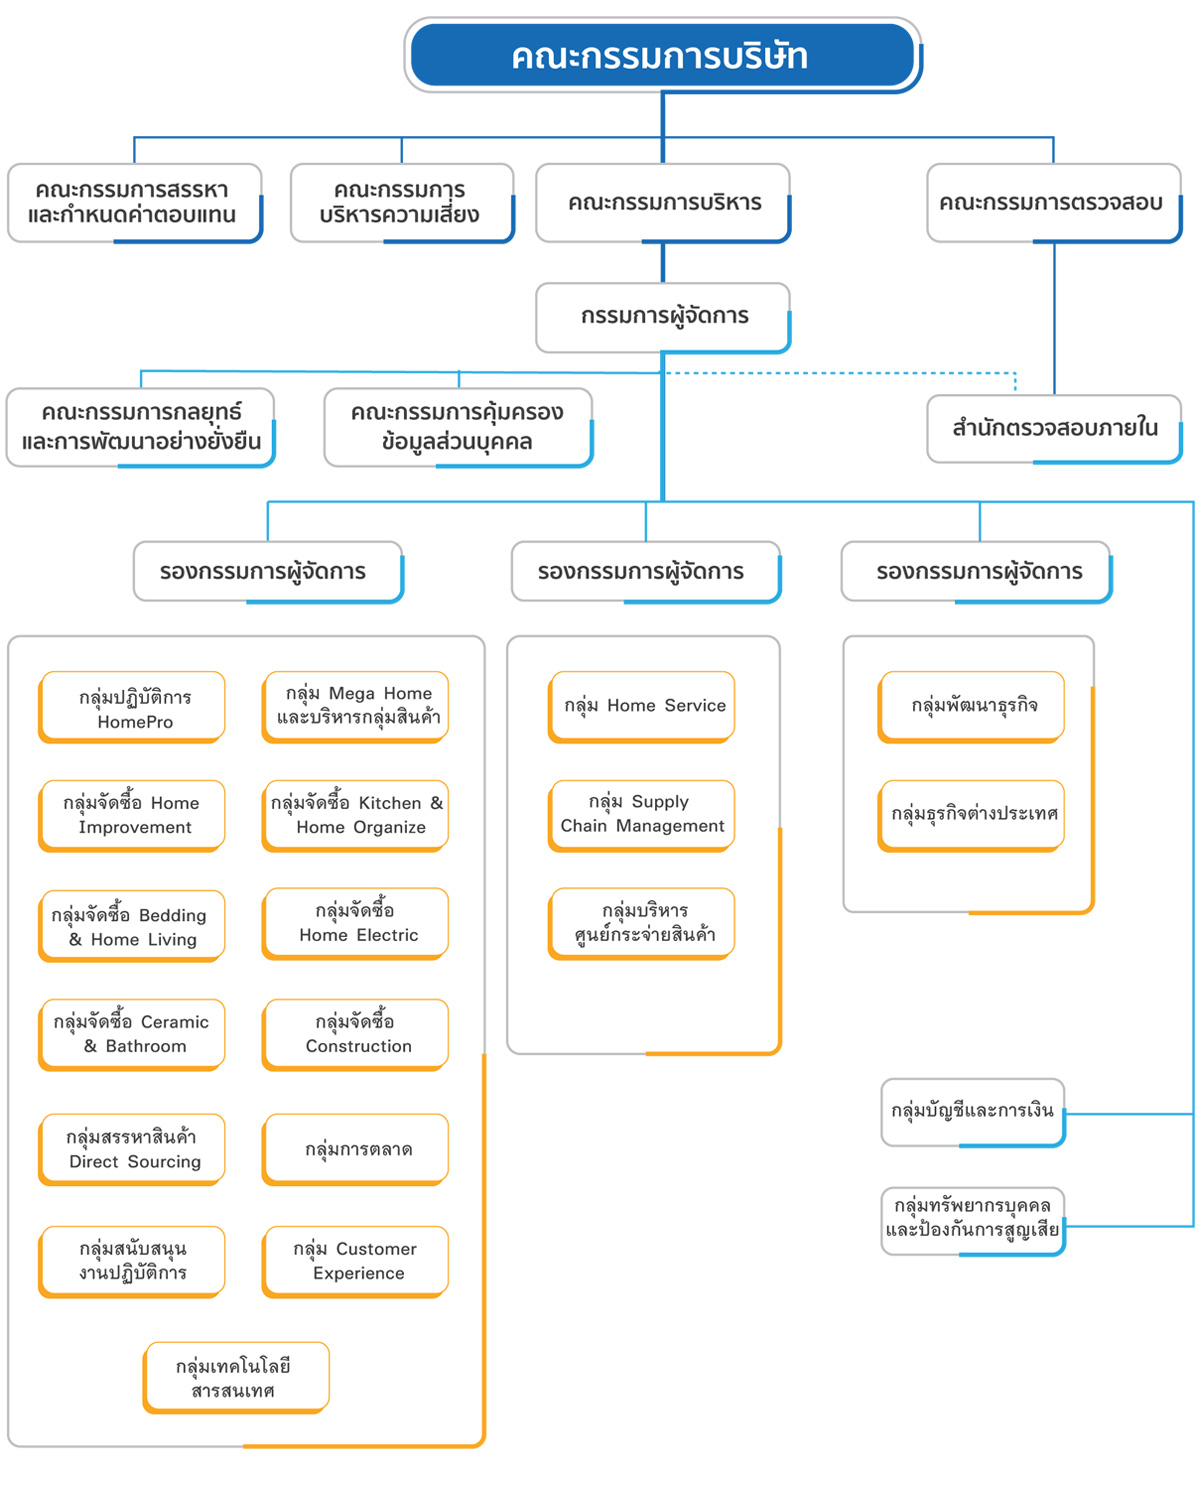
\includegraphics[width=1\textwidth]{homepro-structure}
            \caption{โครงสร้างองค์กรของ บริษัท โฮมโปรดักส์ เซ็นเตอร์ จำกัด (มหาชน)}\label{homepro-structure}
        \end{figure}

    \subsection{ตำแหน่ง และหน้าที่ของงานที่นักศึกษาได้รับมอบหมาย}
        นักศึกษาได้ทำสหกิจในตำแหน่ง PROGRAMMER มีหน้าพัฒนาชุดพัฒนาคำสั่งทดสอบแอปพลิเคชัน E-Catalog ตามเหตุการณ์ที่ผู้ใช้แอปพลิเคชันต้องเจอ และ 
        นำไปทดสอบบน AWS Device Farm อีกทั้งเป็นผู้ร่วมจัดทำคู่มือ การติดตั้งเครื่องมือในการทำพัฒนาชุดคำสั่งทดสอบอัตโนมัติ
        วิธีการสร้างพัฒนาชุดคำสั่งทดสอบอัตโนมัติ

\section{ชื่อ และตำแหน่งของพนักงานที่ปรึกษา}
    \begin{tabular}{ll}
        ชื่อ&{\Exami}\\
        ตำแหน่ง&ผู้จัดการทั่วไป\\
        แผนก&สายบริการส่งเสริมการขาย
    \end{tabular}

\section{ระยะเวลาที่ปฏิบัติงาน}
    เริ่มปฏิบัติงานสหกิจศึกษาตั้งแต่วันที่ 1 มิถุนายน พ.ศ. 2563 ถึง 30 พฤศจิกายน พ.ศ. 2563 รวมเป็นระยะเวลา 26 สัปดาห์

    \chapter{รายละเอียดการปฏิบัติงาน}
\thispagestyle{empty}
\label{chapter:coop-detail}

\section{ตำแหน่ง/หน้าที่ของงานที่ได้รับมอบหมาย}

    \subsection{ตำแหน่งงาน}
        PROGRAMMER
    
    \subsection{หน้าที่ของงานที่ได้รับมอบหมาย}
        \begin{enumerate}
            \item ศึกษาวิธีการทดสอบกับ Flutter แอปพลิเคชันโดยการเพิ่ม key
            \item ศึกษาวิธีการใช้งาน Appium ซึ่งเป็น Framework ที่ช่วยในการทดสอบ แอปพลิเคชัน อัตโนมัติ
            \item ศึกษาวิธีการใช้งาน Appium กับ Flutter ผ่าน Flutter Appium Driver Library
            \item ศึกษาการใช้งาน AWS Device Farm ซึ่งเป็นตัวช่วยจำลองโทรศัพท์ในการทดสอบแอปพลิเคชัน
            \item ศึกษาการพัฒนาชุดคำสั่งทดสอบด้วย NodeJs
            \item ศึกษา HomePro E-Catalog แอปพลิเคชนซึ่งเป็นแอปพลิเคชันที่ต้องนำมาทดสอบ
            \item ออกแบบและพัฒนาชุดคำสั่งทดสอบ
            \item จัดทำคู่มือวิธีการติดตั้ง Appium, AWS Device Farm, NodeJs
            \item จัดทำคู่มือวิธีการพัฒนาชุดคำสั่งทดสอบอัตโนมัติด้วย NodeJs กับ Flutter Appium Driver Library
            \item จัดทำคู่มือวิธีการใช้งาน Appium, AWS Device Farm, NodeJs
        \end{enumerate}

\section{รายละเอียดของโครงงานที่ได้รับผิดชอบ}

    เนื่องจากใน {\Company} เป็นบริษัทขนาดใหญ่จึงจำเป็นต้องมีแอปพลิเคชันหรือระบบภายในไว้ใช้งานจึงมีแผนก ICT Non SAP Front Office
    ไว้คอยพัฒนาระบบหรือแอปพลิเคชันโดยในการจะนำเอาแอปพลิเคชันมาใช้งานหรือแก้ไขต้องเกิดการทดสอบก่อนเสมอเพื่อลดข้อผิดพลาดทางแผนกจึงมอบหมายงาน
    ให้พัฒนาการทดสอบแอปพลิเคชันอัตโนมัติ (Automate Testing) ของแอปพลิเคชัน HomePro E-Catalog ที่เป็นแอปพลิเคชันที่สร้างขึ้นด้วย Flutter เพื่อเป็นต้นแบบไว้คอยนำมาประยุกต์ใช้งานกับ
    แอปพลิเคชันที่จะเกิดขึ้นในอนาคต โดยงานหลักแบ่งได้ 2 อย่างได้แก่
    
    \begin{enumerate}
        \item พัฒนาชุดคำสั่งทดสอบไว้ใช้กับแอปพลิเคชัน HomePro E-Catalog ควบคู่กับ AWS Device Farm
        \item จัดทำเอกสารคู่มือการติดตั้ง, การใช้งาน AWS Device Farm, วิธีการพัฒนาชุดคำสั่งทดสอบ
    \end{enumerate}

    \subsection{ขอบเขตของโครงการ}
        จัดทำชุดคำสั่งทดสอบอัตโนมัติกับแอปพลิเคชันที่ถูกสร้างขึ้นมาด้วย Flutter โดยจะสามารถทดสอบในระบบ Android ได้เท่านั้น โดยกรณีศึกษาจากแอปพลิเคชัน HomePro E-Catalog
        โดยสามรถแบ่งการทดสอบเป็น 34 เหตุการณ์โดยสามารถแบ่งดังนี้
        
        \quad 1. การเขียนทดสอบด้วยกรจับ Element บนหน้าจอโดยไม่ต้องแก้ไขที่ Source Code โดยแบ่งเป็นหน้าจอดังนี้
            \begin{itemize}
                \item หน้าจอ Log-in
                \item หน้าจอ ออกจากระบบ
                \item หน้าจอ รายละเอียดสินค้า
                \item หน้าจอ เปรียบเทียบสินค้า
                \item หน้าจอ รถเข็นสินค้า
                \item หน้าจอ หมวดผู้ใช้งาน
                \item หน้าจอ หมวดเมนู
            \end{itemize}

        \quad 2. การเขียนการทดสอบด้วยการจับ แก้ไขที่ Source Code ของ Flutter โดยใช้ Appium Flutter Driver โดยแบ่งตามหน้าจอดังนี้
            \begin{itemize}
                \item หน้าจอ หมวดสินค้า (Level 3)
                \item หน้าจอ หมวดหมู่ย่อย (Level 2)
                \item หน้าจอ หมวดหมู่ย่อย (Level 1)
            \end{itemize}

        เมื่อพัฒนาชุดคำสั่งเสร็จสิ้นจึงนำไปทดสอบบน AWS Device Farm และจัดทำเอกสารคู่มือวิธีการติดตั้ง, วิธีการพัฒนาชุดคำสั่งทดสอบ, คู่มือการใช้งาน AWS Device Farm

\newpage
\section{รายละเอียดของงานที่ปฏิบัตินอกเหนือจากโครงการที่รับผิดชอบ}
    นอกเหนือจากงานโครงการที่ได้รับผิดชอบยังมีงานอื่นในการช่วยการทำงานของแผนกในฐานะ PROGRAMMER โดยสามารถแบ่งโปรเจ็คที่ได้ทำเป็น 2 ประเภทได้แก่
    
    \subsection{บริการระบบงานขาย Single Sale}
        เป็นระบบที่ใช้ในการยืนยันการซื้อขายสินค้าโดยผู้ใช้งานจะเป็นพนักงานของสาขา {\Company} โดยงานที่ได้รับมอบหมายส่วนใหญ่คือการหาข้อผิดพลาดของระบบและทำการแก้ไข
        ยกตัวอย่าง เช่น การนำข้อมูลออกมาแสดงไม่ถูกต้องจึงต้องไปดูวิธีการนำข้อมูลออกมาและทำการแก้ไขให้ทำงานได้อย่างถูกต้อง หรือ ทำการสร้างหมวดย่อยใหม่เป็นประเภทในการสั่งซื้อสินค้าของลูกค้าเป็นต้น
    
    \subsection{ระบบงานจัดส่งและบริการ Delivery Service}
        เป็นระบบที่ใช้ในการสร้างและยืนยันปิดงานจัดส่งสินค้าโดยผู้ใช้งานจะเป็น พนักงานสาขา, พนักงานจัดส่ง, คอลเซ็นเตอร์ ของ {\Company} โดยงานที่ได้รับมอบหมายส่วนใหญ่คือการหาข้อผิดพลาดของระบบและทำการแก้ไข
        ยกตัวอย่าง เช่น การจัดทีมช่างไปที่บ้านลูกค้าแสดงไม่ถูกต้องจึงต้องทำการแก้ไขให้แสดงได้อย่างถูกต้อง หรือ การปิดงานบางครั้งเป็นงานต่อเนื่องทำหลายวัน
        แต่ระบบได้ปิดงานไปแล้วจึงต้องทำการแก้ไขให้สามารถเก็บการปิดงานเป็นรายวันได้

\section{ลักษณะขั้นตอนกํารทำงาน}
        ลักษณะขั้นตอนการทำงานเป็น รูปแบบ WaterFall มี step การทำอย่างชัดเจนโดยสามารถแบ่งการทำงานดังนี้
        \begin{enumerate}
            \item ศึกษาแอปพลิเคชันที่ต้องการนำมาทดสอบ
            \item ศึกษาวิธีการพัฒนาชุดคำสั่งทดสอบอัตโนมัติ
            \item พัฒนาชุดคำสั่งทำสอบอัตโนมัติแล้วนำไปทดสอบบน AWS Device Farm
            \item จัดทำคู่มือวิธีการติดตั้ง, จัดทำคู่มือวิธีการพัฒนาชุดคำสั่งทดสอบอัตโนมัติด้วย, จัดทำคู่มือวิธีการใช้งาน
            \item รายงานผลการทดลอง
            \item ส่งมอบชุดคำสั่งทดสอบ
        \end{enumerate}


\section{ทฤษฎีที่เกี่ยวข้อง}
    \subsection{การทดสอบซอฟต์แวร์ (Software Testing)}
        Software Testing คือ การทดสอบว่าระบบทำงานได้อย่างถูกต้องหรือไม่ตามวัตถุประสงค์หรือเปล่าและสามารถระบุข้อผิดพลาดเพื่อสามารถนำไปแก้ไขได้
        ก่อนการนำไปจัดส่งซึงการทำการทดสอบซอฟต์แวร์นั้นมีความสำคัญมากเนื่องจากการเจอ ข้อผิดพลาดในซอฟต์แวร์นั้นมีค่าใช้จ่ายที่สูงหากเกิดขึ้นตอนนำจัดส่งไปแล้ว
        โดยการทดสอบซอฟต์แวร์แบ่งเป็นได้ 2 ประเภทได้แก่
        \begin{enumerate}
            \item Manual Testing คือ การทดสอบที่ไม่ใช้เครื่องมืออัตโนมัติหรือ Script เลยจะทดสอบตาม Test Plan, Test Case หรือ Test Scenarios ด้วยมือของผู้ทดสอบเอง
            \item Automation Testing คือ การทดสอบอัตโนมัติด้วยการเขียนชุดคำสั่งในการทดสอบ (Script)
        \end{enumerate}
        \begin{figure}[H]
            \centering
            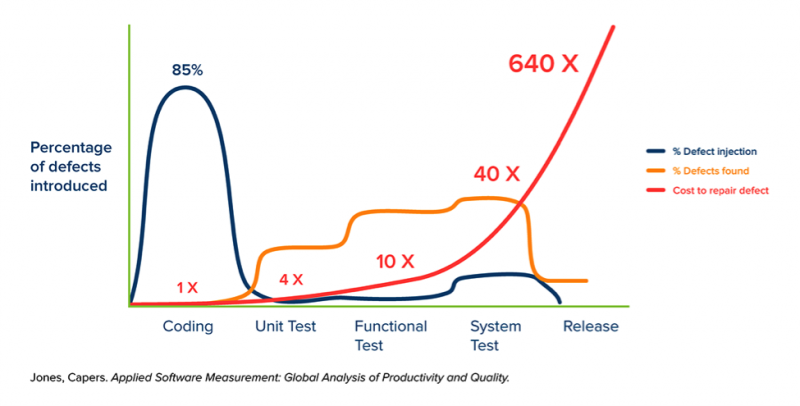
\includegraphics[width=1\textwidth]{cost-of-fixing-bug}
            \caption{ค่าใช้จ่ายการแก้ข้อผิดพลาดที่แปรผันตามขั้นตอนของการพัฒนาซอฟต์แวร์}\label{cost-of-fixing-bug}
        \end{figure}

    \subsection{การทดสอบอัตโนมัติ (Automation Testing)}
        Automation Testing คือ การทดสอบแบบอัตโนมัติโดยการเขียนชุดคำสั่งทดสอบแทนแบบเดิมที่ใช้การทดสอบก้วยมือ ยกตัวอย่าง เช่น
        การทดสอบซอฟต์แวร์แบบเดิมด้วยการใช้มือจะต้องกรอกแบบสอบถามในแอปพลิเคชันในวันแรกและเจอข้อผิดพลาดวันถัดไปนักพัฒนาแอปพลิเคชัน
        ก็ปรับปรุงแอปพลิเคชันมาใหม่ให้ไปทดสอบกรอกแบบเดิมอีกและอาจเจอข้อผิดพลาดใหม่หรือไม่เจอแต่ถ้าหากเกิดการแก้ไขหรือเปลี่ยนแปลงกับ
        ตัวแอปพลิเคชันแล้วต้องทำการทดสอบใหม่อยู่ตลอดซึ่งเป็นการทำงานรูปแบบเดิม แต่การทำ Automation Testing จะมาช่วยแก้ปัญหาโดย
        การเขียนชุดคำสั่งเพื่อมากรอกแบบทดสอบให้ในแอปพลิเคชันซึ่งกำหนดไว้ว่าสิ่งที่ถูกต้องควรจะเป็นอย่างไรและหากไม่ถูกต้องไม่ถูกต้องอย่างไร
        โดยจะเป็นการทำแบบอัตโนมัติด ดังนั้นข้อดีของ Automation Testing ได้แก่
        \begin{itemize}
            \item[-] ผลตอบรับที่ไวขึ้นต่อรอบการพัฒนาหรือแก้ไขแอปพลิเคชัน
            \item[-] สามารถประหยัดค่าใช้จ่ายในการทดสอบได้
            \item[-] สามารถทดสอบได้อย่างคลอบคลุมมากขึ้น
            \item[-] สามารถนำแอปพลิเคชันมาส่งมอบได้เร็วขึ้น
            \item[-] เพิ่มความแม่นยำในการทดสอบมากขึ้น 
            \item[-] กำจัดการทดสอบที่จะผิดพลาดที่เกิดจากมนุษย์ 
        \end{itemize}
        ในปัจจุบันมีเครื่องมือช่วยในการทำ Automation Testing มากมายยกตัวอย่างดังนี้
        \begin{enumerate}

            \item Katalon Studio คือ เครื่องมือตัวหนึ่งในการช่วยทำ Test Automation ของ Mobile Applications ซึ่งสามารถทดสอบได้ทั้ง
            Android และ IOS
            \begin{figure}[H]
                \centering
                
\includegraphics[width=0.3\textwidth]{katalon-studio}
                \caption{ตราตราสัญลักษณ์ Katalon Studio}\label{katalon-studio}
            \end{figure}

            \item Selenium คือ Software Testing Framework ที่มีประสิทธิภาพไว้ใช้สำหรับเขียนชุดคำสั่งทดสอบ Web Applications ซึ่งเป็นแบบ Open Source สามารถเขียนได้ด้วยหลายภาษา เช่น Java, Python, \texttt(C\#), Javascript, PHP, Perl 
            \begin{figure}[H]
                \centering
                
\includegraphics[width=0.5\textwidth]{selenium}
                \caption{ตราตราสัญลักษณ์ Selenium}\label{selenium}
            \end{figure}

            \item Micro Focus UFT คือ หนึ่งใน Software ที่มีประสิทธิภาพที่สุดสำหรับการทำการทดสอบแบบ Functional Testing สามารถสร้าง Test และแก้ไขได้อย่างรวดเร็วไปจนถึงสามารถนำเทคโนโลยี Object Recognition, Image-based Automation และ Machine Driven Regression Testing เข้ามาใช้ช่วยในการทำงาน
            แต่เสียค่าใช้จ่ายแต่มีให้ทดลองใช้งานฟรี 60 วัน
            \begin{figure}[H]
                \centering
                
\includegraphics[width=0.20\textwidth]{uft}
                \caption{ตราตราสัญลักษณ์ Micro Focus UFT}\label{uft}
            \end{figure}

            \item TestComplete คือ หนึ่งใน Software ที่มีประสิทธิภาพที่สุดสำหรับการทำการทดสอบ Desktop, Mobile และ Web Applications ตามชุดคำสั่งที่เขียนได้ด้วย
            ภาษา Python, JavaScript, VBScript และอื่นๆ
            \begin{figure}[H]
                \centering
                
\includegraphics[width=0.5\textwidth]{test-com}
                \caption{ตราตราสัญลักษณ์ TestComplete}\label{test-com}
            \end{figure}


        \end{enumerate}

    \subsection{Appium}
        Appium คือ เครื่องมือสำหรับการทำ Automation Testing เป็นรุปแบบ Open Source ไว้สำหรับทดสอบ Native, Mobile Web, Hybrid
        , Android, IOS และ Windows Desktop การใช้ Appium จะเป็น Cross Platform หมายความว่าจะทำให้สามารถเขียน
        โดยใช้ API เดียวกันซึ่งจะช่วยให้สามารถใช้โค้ดซ้ำระหว่างอุปกรณ์ที่ทดสอบได้ IOS, Android, Window การทำงานจะสื่อสารระหว่าง Driver กับ Appium ผ่าน JSON โดยรองรับการเขียนได้หลายภาษา
        เช่น Python, Java, JavaScript(NodeJS), Ruby 
        \begin{figure}[H]
            \centering
            
\includegraphics[width=0.3\textwidth]{appium}
            \caption{ตราตราสัญลักษณ์ Appium}\label{appium}
        \end{figure}

        Driver ที่สามารถใช้กับ Appium ได้แก่
        \begin{itemize}
            \item XCUITest Driver (for iOS and tvOS apps)
            \item Espresso Driver (for Android apps)
            \item UiAutomator2 Driver (for Android apps)
            \item Windows Driver (for Windows Desktop apps)
            \item Mac Driver (for Mac Desktop apps)
        \end{itemize}

        \begin{figure}[H]
            \centering
            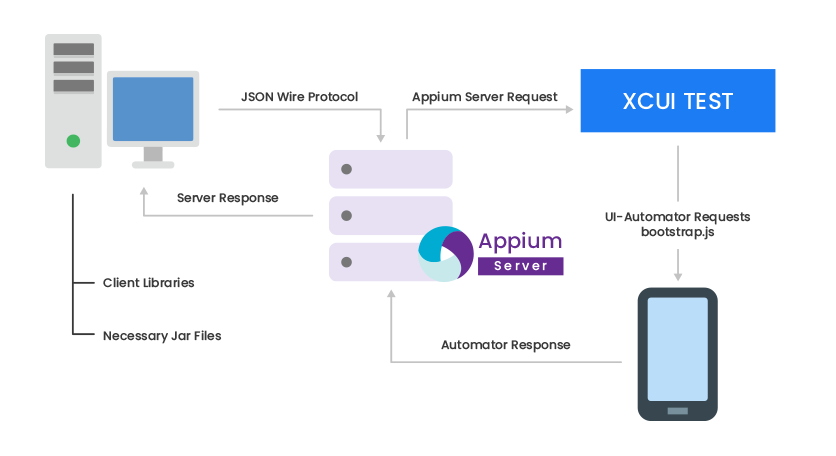
\includegraphics[width=1\textwidth]{appium-arc}
            \caption{โครงสร้างการทำงานของ Appium}\label{appium-arc}
        \end{figure}

        นอกเหนือจากนี้ Appium ยังสามารถใช้งานร่วมกับ AWS Device Farm ได้

    \subsection{API}
        API (Application Programming Interface) คือ วิธีการติดต่อสื่อสารระหว่างแอปพลิเคชันไม่ว่าแอปพลิเคชันนั้นจะรันอยู่บนอุปกรณ์ใด เช่นคอมพิวเตอร์ โทรศัพท์มือถือ หรือเฟิร์มแวร์ในอุปกรณ์เครื่องใช้ต่างๆ โดยที่แอปพลิเคชันฝั่งหนึ่งเป็นผู้ขอใช้บริการหรือขอข้อมูลจากแอปพลิเคชันอีกฝั่งหนึ่งซึ่งเป็นผู้ให้บริการ การติดต่อสื่อสารระหว่างแอปพลิเคชันดังกล่าวเป็นไปโดยอัตโนมัติตามที่ได้กำหนดไว้

    \subsection{AWS Device Farm}
         AWS คือ Amazon Web Services เป็นคลาวด์แพลตฟอร์มที่มีคนนำมาใช้มากที่สุดในโลกที่มีการบริการ 175 บริการ
         โดยองค์กรขนาดใหญ่หรือสตาร์ทอัพก็เริ่มหันมาใช้ AWS เพื่อลดค่าใช้จ่ายและความคล่องตัว

        \begin{figure}[H]
            \centering
            
\includegraphics[width=0.5\textwidth]{aws}
            \caption{ตราสัญลักษณ์ Amazon Web Service (AWS)}\label{aws}
        \end{figure}

        AWS Device Farm คือ บริการหนึ่งของ AWS เป็นบริการไว้ทดสอบแอปพลิเคชันเพื่อปรับปรุงคุณภาพแอปพลิเคชันหรือระบบต่างๆ
        โดย AWS Device Farm จะทดสอบแอปพลิเคชันหรือระบบใน Desktop, Browser หรืออุปกรณ์มือถือที่หลากหลายทั้งในระบบปฎิบัติการ Android และ IOS พร้อมกันเพื่อช่วย
        ให้ชุดทดสอบรวดเร็วขึ้น หลากหลายมากขึ้น และพร้อมสร้างวีดีโอและบันทึกเพื่อช่วยให้หาปัญหาของระบบหรือแอปพลิเคชันได้ไวยิ่งขึ้น

        \begin{figure}[H]
            \centering
            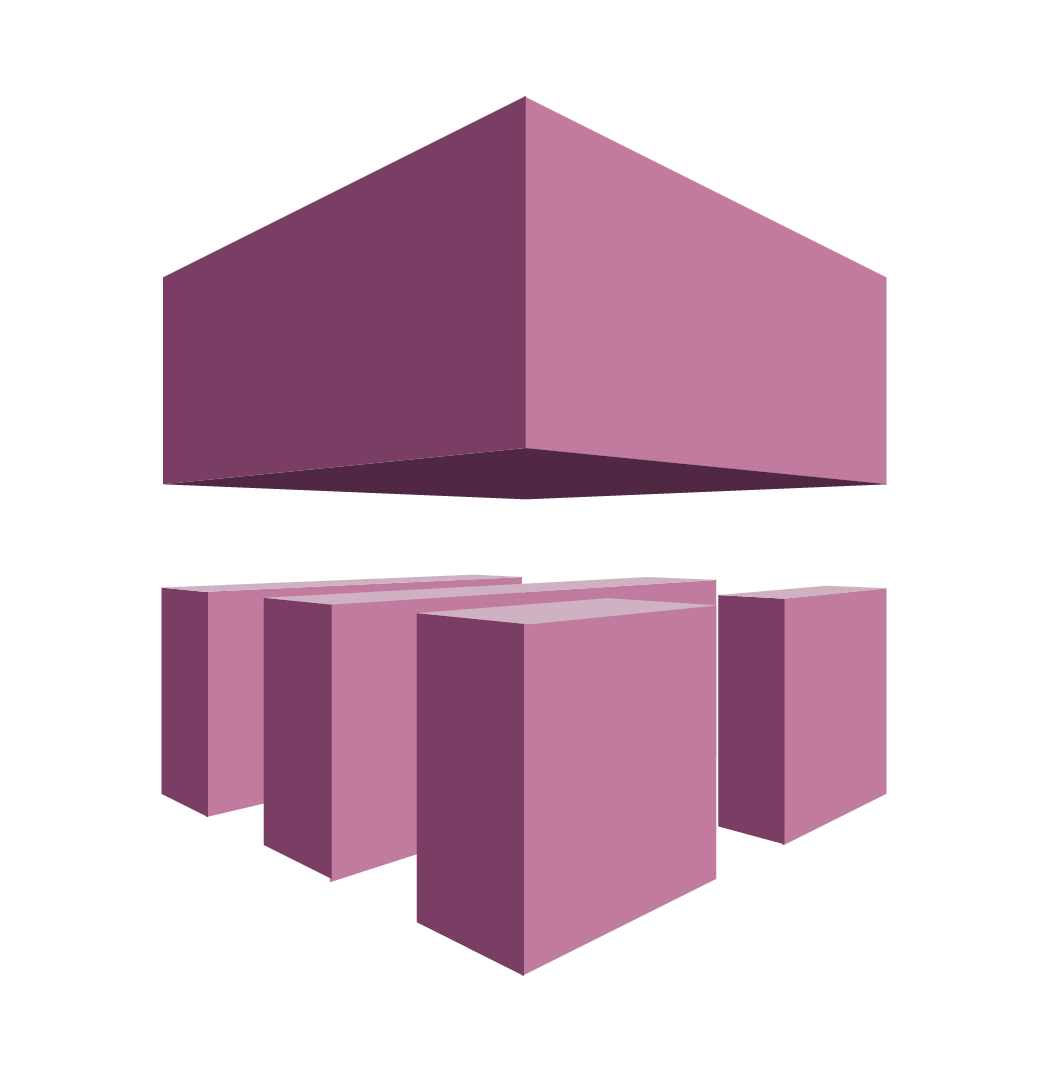
\includegraphics[width=0.25\textwidth]{amazon-device-farm}
            \caption{ตราสัญลักษณ์ AWS Device Farm}\label{amazon-device-farm}
        \end{figure}

    \subsection{Node.Js}
        Node.Js คือ JavaScript runtime environment เป็น OpenSource คือการที่สามารถนำเอา JavaScript มาใช้งานแบบภาษาอื่นบน
        Windows, Linux หรือ Mac ได้แบบไม่เสียค่าใช้จ่ายหากติดตั้ง Node.js จะสามารถเขียนโปรแกรมด้วยภาษา JavaScript เหมือนกับ Java, \texttt(C\#), Python
        ซึ่งหลักๆแล้วจะนำมาทำเป็น backend server นอกจากนี้ Node.Js ยังมี NPM (Node Package Manager) เป็นตัวที่ใช้สำหรับการดาวน์โหลด
        library ภายนอกมาใช้โดยติดตั้งเพียงพิมพ์ `npm install <ชื่อ library>` เช่น mocha, express, chai เป็นต้น

        \begin{figure}[H]
            \centering
            
\includegraphics[width=0.3\textwidth]{node}
            \caption{ตราสัญลักษณ์ Node.JS}\label{node}
        \end{figure}
        

    \subsection{Flutter}
        Flutter คือ Framework แบบ OpenSource ที่ถูกพัฒนาโดย Google มีไว้เพื่อใช้สร้าง UserInterface สำหรับ Mobile Application ที่สามารถทำงานข้ามแพลตฟอร์มได้ทั้ง IOS และ Android คือเขียนโปรแกรมหนึ่งครั้งสามารถนำมาใช้ได้ทั้งสองแพลตฟอร์มโดยภาษาที่ Flutter ใช้คือภาษา Dart
        โดยจุดเด่นของ Flutter คือระบบ Hot Reload จะเข้ามาช่วยในส่วนของการ reload สามารถพัฒนาแอปพลิเคชัน ในส่วน UserInterface มีความรวดเร็วมากขึ้นอีกทั้งยังมีความสวยงามแบบ
        Material Design

        \begin{figure}[H]
            \centering
            
\includegraphics[width=0.5\textwidth]{flutter}
            \caption{ตราสัญลักษณ์ Flutter}\label{flutter}
        \end{figure}

    \subsection{Appium Flutter Driver}
        Appium Flutter Driver คือ เครื่องมือช่วยในการทำ Automation Test กับแอปพลิเคชันที่สร้างมาจาก Flutter เป็นส่วนหนึ่งในการใช้งานกับ Appium โดย Appium Flutter Driver จะใช้ Dart Service Protocol เพื่อส่ง API ไปเรียกใช้การ Test ของ Flutter ที่ทั่วไปต้องเขียนเป็นภาษา Dart แต่ถ้าใช้ library นี้จะเขียนภาษาตามที่ Appium มีได้เลย

        \begin{figure}[H]
            \centering
            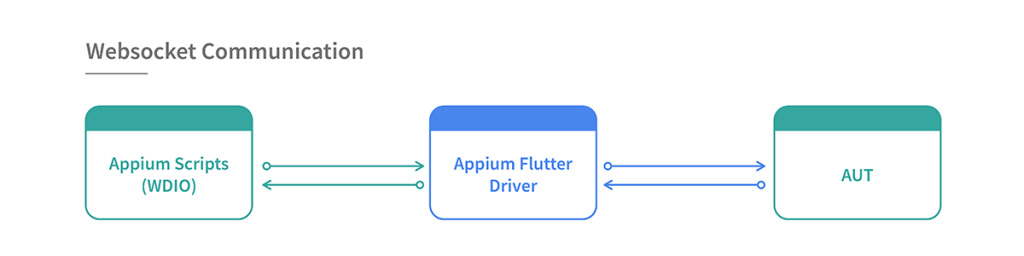
\includegraphics[width=1\textwidth]{appium-flutter}
            \caption{โครงสร้างการทำงานของ Appium Flutter Driver}\label{appium-flutter}
        \end{figure}

    \subsection{"Wd"}
        Wd คือ library JavaScript ที่ใช้ในการทำ Automation Test ใน NodeJS โดยที่สามารถทำงานร่วมกับ Selenium และ Appium ใช้จับ element แบบ xpath

    \subsection{WebdriverIO}
        WebdriverIO คือ library JavaScript ที่ใช้ในการทำ Automation Test ใน NodeJS โดยที่สามารถทำงานร่วมกับ Selenium และ Appium ได้

    \subsection{Xpath}
        Xpath คือ ตัวชี้ทางในภาษาต่างๆ (เช่น XML, HTML) เพื่อแสดง Root ของเส้นทางการเข้าถึงข้อมูลตามลำดับชั้น
        
    \subsection{Mocha}
        Mocha คือ library JavaScript ที่ใช้ใน NodeJs เพื่อทำการทดสอบอัตโนมัติแบบ Asynchronous Testing ได้ง่ายขึ้นโดยการแสดงผลลัพธ์ที่ผิดพลาดอย่างง่ายและชัดเจนตาม Test Case

    \subsection{Chai}
        Chai คือ library JavaScript ที่ใช้ใน NodeJs ทำหน้าที่เปรียบที่ค่าผลลัพธิ์ที่ได้จากการทดสอบกับผลลัพธ์ที่ควรจะเป็นโดยเป็นรูปแบบที่เข้าใจง่าย

    \subsection{Git}
        Git คือ Vesion Control เป็นตัวที่ใช้จัดเก็บและคอยดูการเปลี่ยนแปลงกับไฟล์ชนิดใดก็ได้เมื่อจัดเก็บไฟล์เข้าไปในระบบของ Git แล้วจะเรียกว่า Git Repository ซึ่งสำรองข้อมูลของ Source Code สามารถย้อนกลับไปเวอร์ชั่นใดก่อนหน้าและดูรายละเอียดการเปลี่ยนแปลงของแต่ละเวอร์ชั่นได้

        \begin{figure}[H]
            \centering
            
\includegraphics[width=0.3\textwidth]{git-logo}
            \caption{ตราสัญลักษณ์ Git}\label{git-logo}
        \end{figure}

    \subsection{Visual Studio Code}
        Visual Studio Code คือ Editor ตัวหนึ่งที่สร้างมาเพื่ออำนวยความสะดวกแก่โปรแกรมเมอร์มีธีมและรองรับรูปแบบการเขียนได้หลายภาษาอีกทั้งยังมีตัวช่วยในการเขียนโปรแกรมต่างๆ เช่น Bracket Matcher, Live Server เป็นต้น

        \begin{figure}[H]
            \centering
            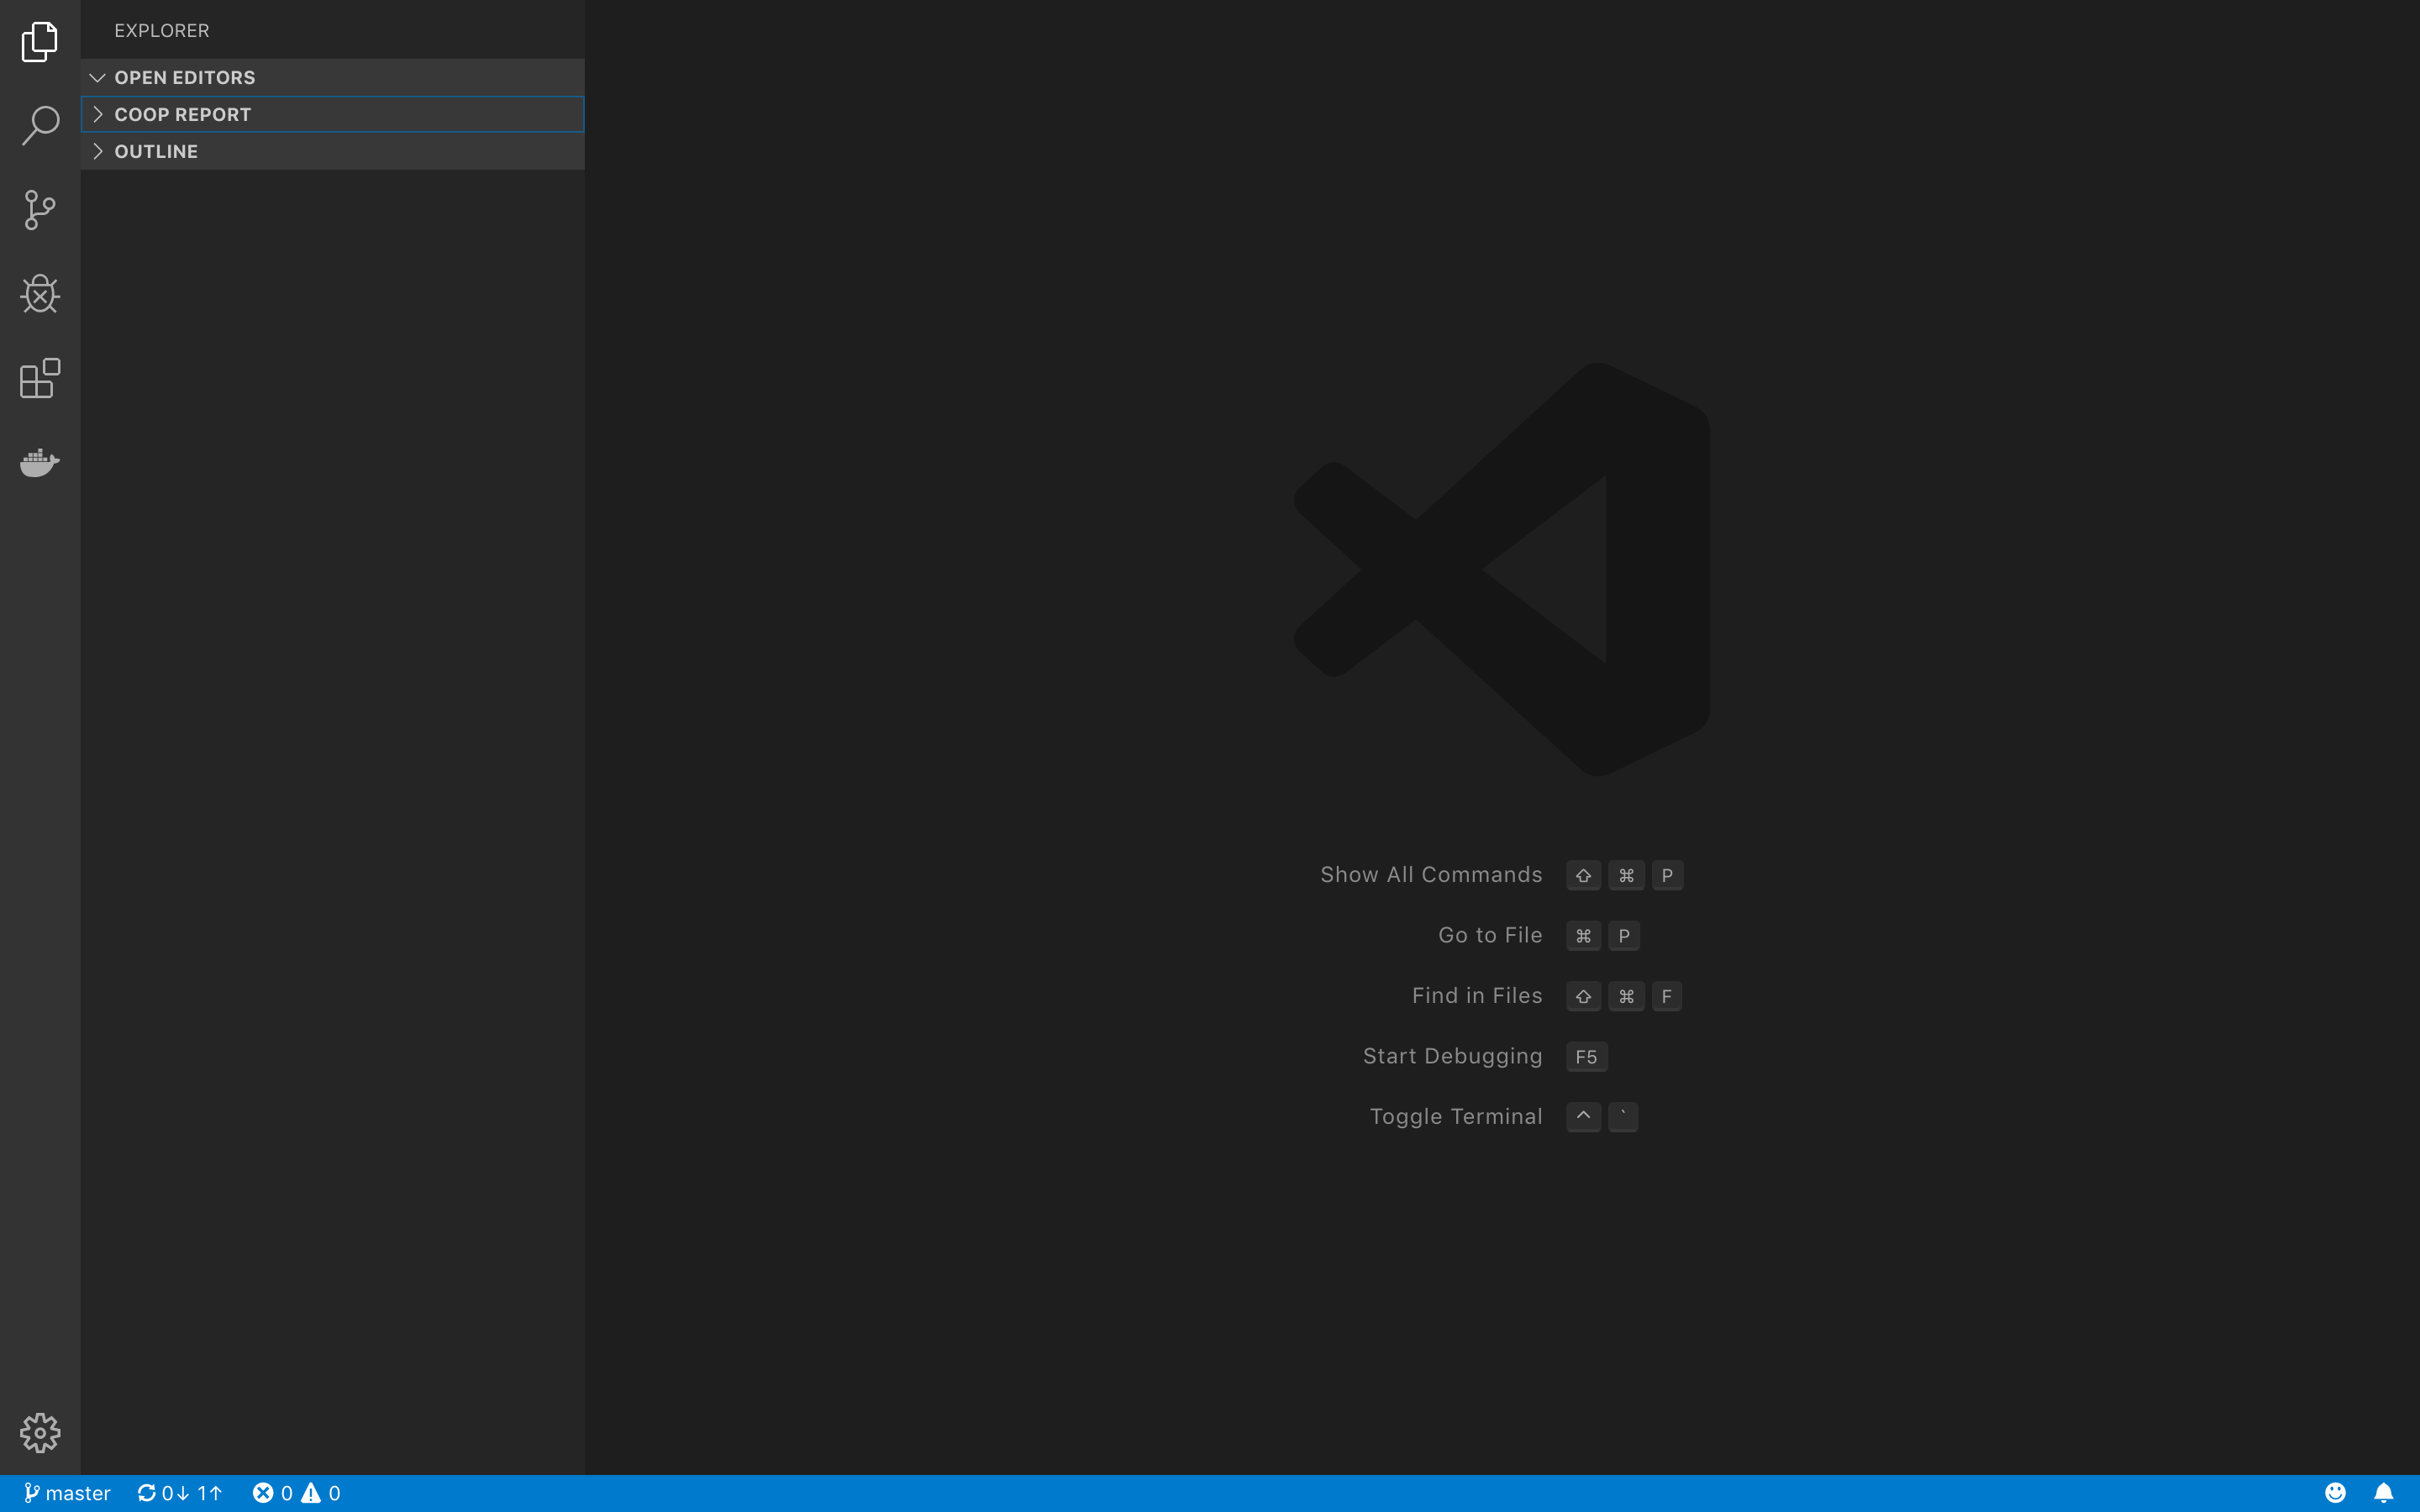
\includegraphics[width=0.2\textwidth]{visual-studio-code}
            \caption{ตราสัญลักษณ์ Visual Studio Code}\label{visual-studio-code}
        \end{figure}
    \chapter{สรุปผลการปฎิบัติงาน}
\thispagestyle{empty}
\label{chapter:designAndDevelop}

\titleformat{\paragraph}
{\normalfont\normalsize\bfseries}{\theparagraph}{1em}{}
\titlespacing*{\paragraph}
{0pt}{3.25ex plus 1ex minus .2ex}{1.5ex plus .2ex}

\section{ผลการศึกษาแอปพลิเคชัน HomePro E-Catalog}
โฮมโปร อีแค็ตตาล็อค เป็น แอปพลิเคชันของโฮมโปรที่นำมาใช้ภายในบริษัทไว้ให้พนักงานขายของโฮมโปรที่สาขาสามารถช่วยเพิ่มประสิทธิภาพในการขายได้โดยจะมีเหตุการณ์ที่สามารถช่วยในการ
ขายสามารถมีดังนี้

\begin{enumerate}
    \item \textbf{การแสดงสินค้าที่ลูกค้าสนใจ}\newline ตัวแอปพลิเคชันสามารถแสดงสินค้าตามที่ผู้ใช้คนหาได้อีกทั้งแบ่งเป็นหมวดแล้วกรองได้หลายวิธี
    ยกตัวอย่างเช่น หากลูกค้าต้องการซื้อโต๊ะทำงานเมื่อลูกค้าถามถึงโต๊ะทำงานพนักงานขายจะเปิดแอปพลิเคชันและทำการแสดงให้ลูกค้าดูแบบของโต๊ะทำงานของที่ {\Company}
    จำหน่ายและราคาที่สามารถเปรียบเทียบราคาได้
    \item \textbf{การแสดงสต๊อคสินค้า}\newline ตัวแอปพลิเคชันสามารถแสดงสต๊อคสินค้าของสาขาที่มีสินค้าได้ยกตัวอย่างเช่นหากลูกค้ามาตามหาสินค้าแล้วไม่พบที่ชั้นวางหรือสินค้านี้ในสาขานี้หมดสามารถให้พนักงานเข้าแอปพลิเคชัน
    ค้นหาสินค้าแล้วดูสต๊อคสินค้าของสินค้าที่ต้องการได้ว่าสาขาใดมีบ้างทำให้ไม่เสียลูกค้า
    \item \textbf{การสั่งซื้อสินค้า}\newline ตัวสินค้าสามารถสั่งซื้อสินค้าได้เลยเพียงแค่กรอกเบอร์มือถือของลูกค้าก็จะเปรียบเสมือนลูกค้าได้นำสินค้าเข้าตะกร้าทำให้ปิดการขายได้รวดเร็วมากขึ้น
\end{enumerate}

\subsection{เหตุการณ์ (Senario) ในการพัฒนาชุดคำสั่งทดสอบจากการศึกษา} 
    \begin{enumerate}
        \item หน้า Log-in : กรอกรหัสพนักงาน และ รหัสผ่าน ถูกต้อง
        \item หน้า Log-in : กรอกรหัสพนักงาน หรือ รหัสผ่าน ไม่ถูกต้อง
        \item ออกจากระบบ : ต้องการออกจากระบบด้วยแทบ "ผู้ใช้งาน" ใน BottomNavigationBar
        \item ออกจากระบบ : ต้องการออกจากระบบด้วยแทบ "เมนู" ใน BottomNavigationBar
        \item หน้าหลัก - หมวดหมู่หลัก (Level 3) : ตรวจสอบการแสดงหมวดหมู่สินค้า
        \item หน้าหลัก - หมวดหมู่หลัก (Level 3) : ปุ่มค้นหา
        \item หน้าหลัก - หมวดหมู่ย่อย (Level 2) : ตรวจสอบการแสดงหมวดหมู่สินค้า
        \item หน้าหลัก - หมวดหมู่ย่อย (Level 2) : ดูทั้งหมด
        \item หน้าหลัก - หมวดหมู่ย่อย (Level 1) : เลือกตัวกรอง – ตัวกรองหมวดสินค้า
        \item หน้าหลัก - หมวดหมู่ย่อย (Level 1) : เลือกตัวกรอง – ตัวกรองแบนด์
        \item หน้าหลัก - หมวดหมู่ย่อย (Level 1) : ตรวจสอบการแสดงหมวดหมู่สินค้า Default
        \item หน้าหลัก - หมวดหมู่ย่อย (Level 1) : ตัวเลือก จัดเรียง – เรียงจากราคาน้อยไปหามาก
        \item หน้าหลัก - หมวดหมู่ย่อย (Level 1) : ตัวเลือก จัดเรียง – เรียงจากราคามากไปหาน้อย
        \item หน้าหลัก - หมวดหมู่ย่อย (Level 1) : ตัวเลือก เปรียบสินค้าหน้าหลัก
        \item หน้าหลัก - รายละเอียดสินค้า (Detail) : ตรวจสอบรายละเอียดของสินค้า 
        \item หน้าหลัก - รายละเอียดสินค้า (Detail) : ปุ่มเปรียบเทียบ หน้า Detail
        \item หน้าหลัก - รายละเอียดสินค้า (Detail) : แถบรายละเอียดสินค้า
        \item หน้าหลัก - รายละเอียดสินค้า (Detail) : แถบข้อมูลจำเพาะ
        \item หน้าหลัก - รายละเอียดสินค้า (Detail) : แถบโปรโมชั่นหน้าหลัก
        \item หน้าหลัก - รายละเอียดสินค้า (Detail) : ปุ่ม สต๊อกสินค้า
        \item หน้าหลัก - รายละเอียดสินค้า (Detail) : ปุ่ม สต๊อกสินค้าเพิ่มเติม
        \item หน้าจอเปรียบเทียบสินค้า : เปรียบเทียบ
        \item หน้าจอเปรียบเทียบสินค้า : เปรียบเทียบมากกว่า 3 รายการ
        \item หน้าจอเปรียบเทียบสินค้า : ยกเลิกตัวที่เปรียบเทียบบางรายการ
        \item หน้าจอเปรียบเทียบสินค้า : ยกเลิกการเปรียบเทียบทั้งหมด
        \item หน้าจอเปรียบเทียบสินค้า : ปุ่ม เพิ่มลงรถเข็น
        \item รถเข็นสินค้า – แก้ไขรายการสินค้า : แก้ไขจำนวนสินค้า (เพิ่ม-ลด)
        \item รถเข็นสินค้า – แก้ไขรายการสินค้า : แก้ไขจำนวนสินค้า (เพิ่ม) โดยให้มี QTY รวมกันเกิน 999
        \item รถเข็นสินค้า – แก้ไขรายการสินค้า : ลบรายการสินค้า
        \item รถเข็นสินค้า – สร้างใบคำสั่งซื้อ : สร้างใบคำสั่งซื้อ โดยใช้เบอร์โทรที่ไม่ใช่เบอร์มือถือ
        \item รถเข็นสินค้า – สร้างใบคำสั่งซื้อ : สร้างใบคำสั่งซื้อ โดยใช้เบอร์โทรที่เบอร์มือถือถูกต้อง
        \item ผู้ใช้งาน : ข้อมูลผู้เข้าใช้งาน
        \item เมนู – เลือกหมวดสินค้า : การค้นหาสินค้าจากการเลือกหมวดสินค้า
        \item เมนู – เลือกตามแบรนด์ : การค้นหาสินค้าจากการเลือกแบรนด์สินค้า
        \item เมนู – ภาษา : การเลือกภาษา
    \end{enumerate}

\newpage
\section{ผลการทดสอบด้วยการจับ Element บนหน้าจอโดยไม่ต้องแก้ไขที่ Source Code}
    เป็นวิธีการที่จับ Element โดยการใช้ Xpath และ Accessibility id บนหน้าจอโดยใช้ Appium ซึ่งวิธีการนี้ผู้พัฒนาชุดคำสั่งทดสอบไม่ต้องเข้าไปแก้ไขที่ Source Code ของแอปพลิเคชันดังตัวอย่างด้านล่าง
    \begin{figure}[H]
        \centering
        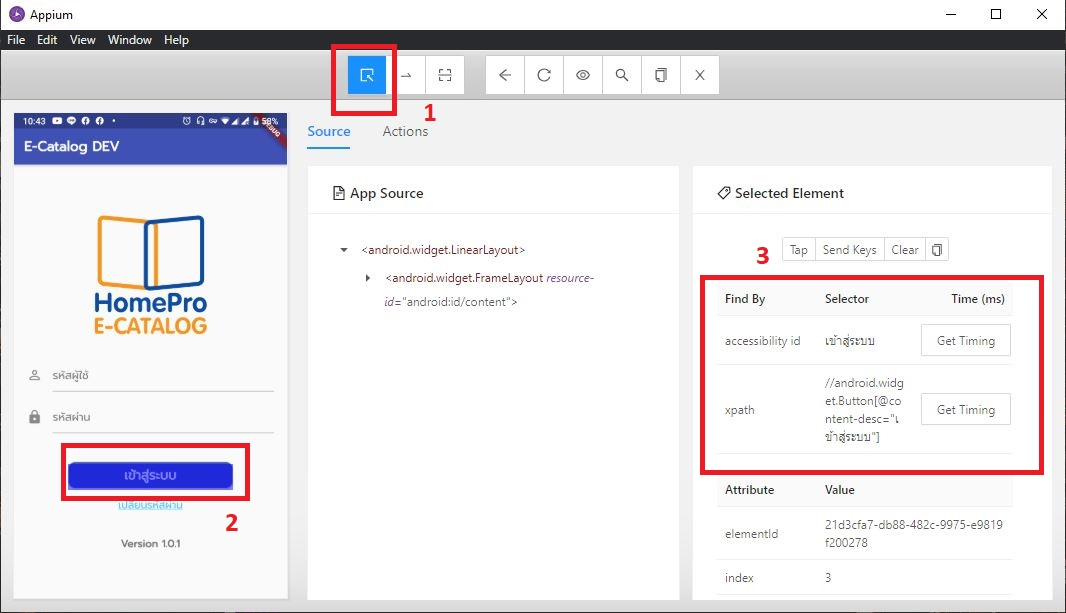
\includegraphics[width=1\textwidth]{xpathway}
        \caption{การดูค่า Element ด้วย Appium}\label{xpathway}
    \end{figure}

    จากรูปที่ 3.1 จะเห็นได้ว่าเมื่อชี้ที่ภาพในหมายเลข 2 จะปรากฎช่องด้านขวาซึ่งเป็นชื่อและค่าของ Element ที่อยู่ในช่องด้านขวาในหมายเลข 3 นำมาใช้งานต่อ

    \begin{figure}[H]
        \centering
        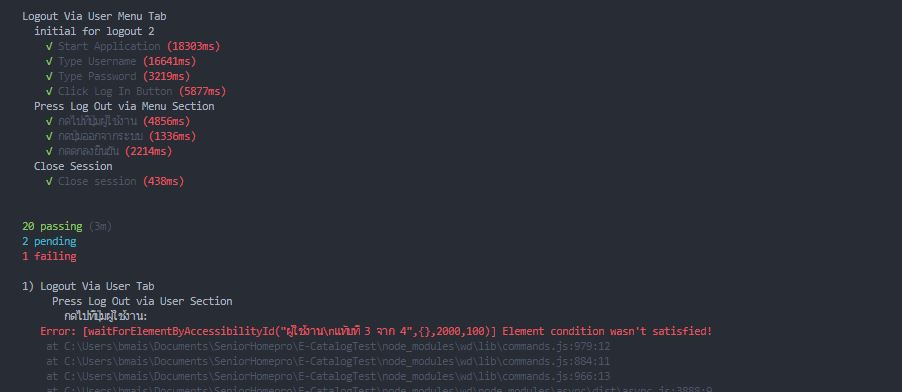
\includegraphics[width=1\textwidth]{output1}
        \caption{ตัวอย่างการแสดงผลของการทดสอบ}
        \label{result}
    \end{figure}

    จากรูป 3.2 เป็นรูปสรุปผลการทดสอบว่ามีผ่านจำนวนทั้งหมดเท่าไหร่ ผิดผลาด (Test Fail) เท่าไร่และทำไมถึงผิดพลาด        

    \begin{figure}[H]
        \centering
        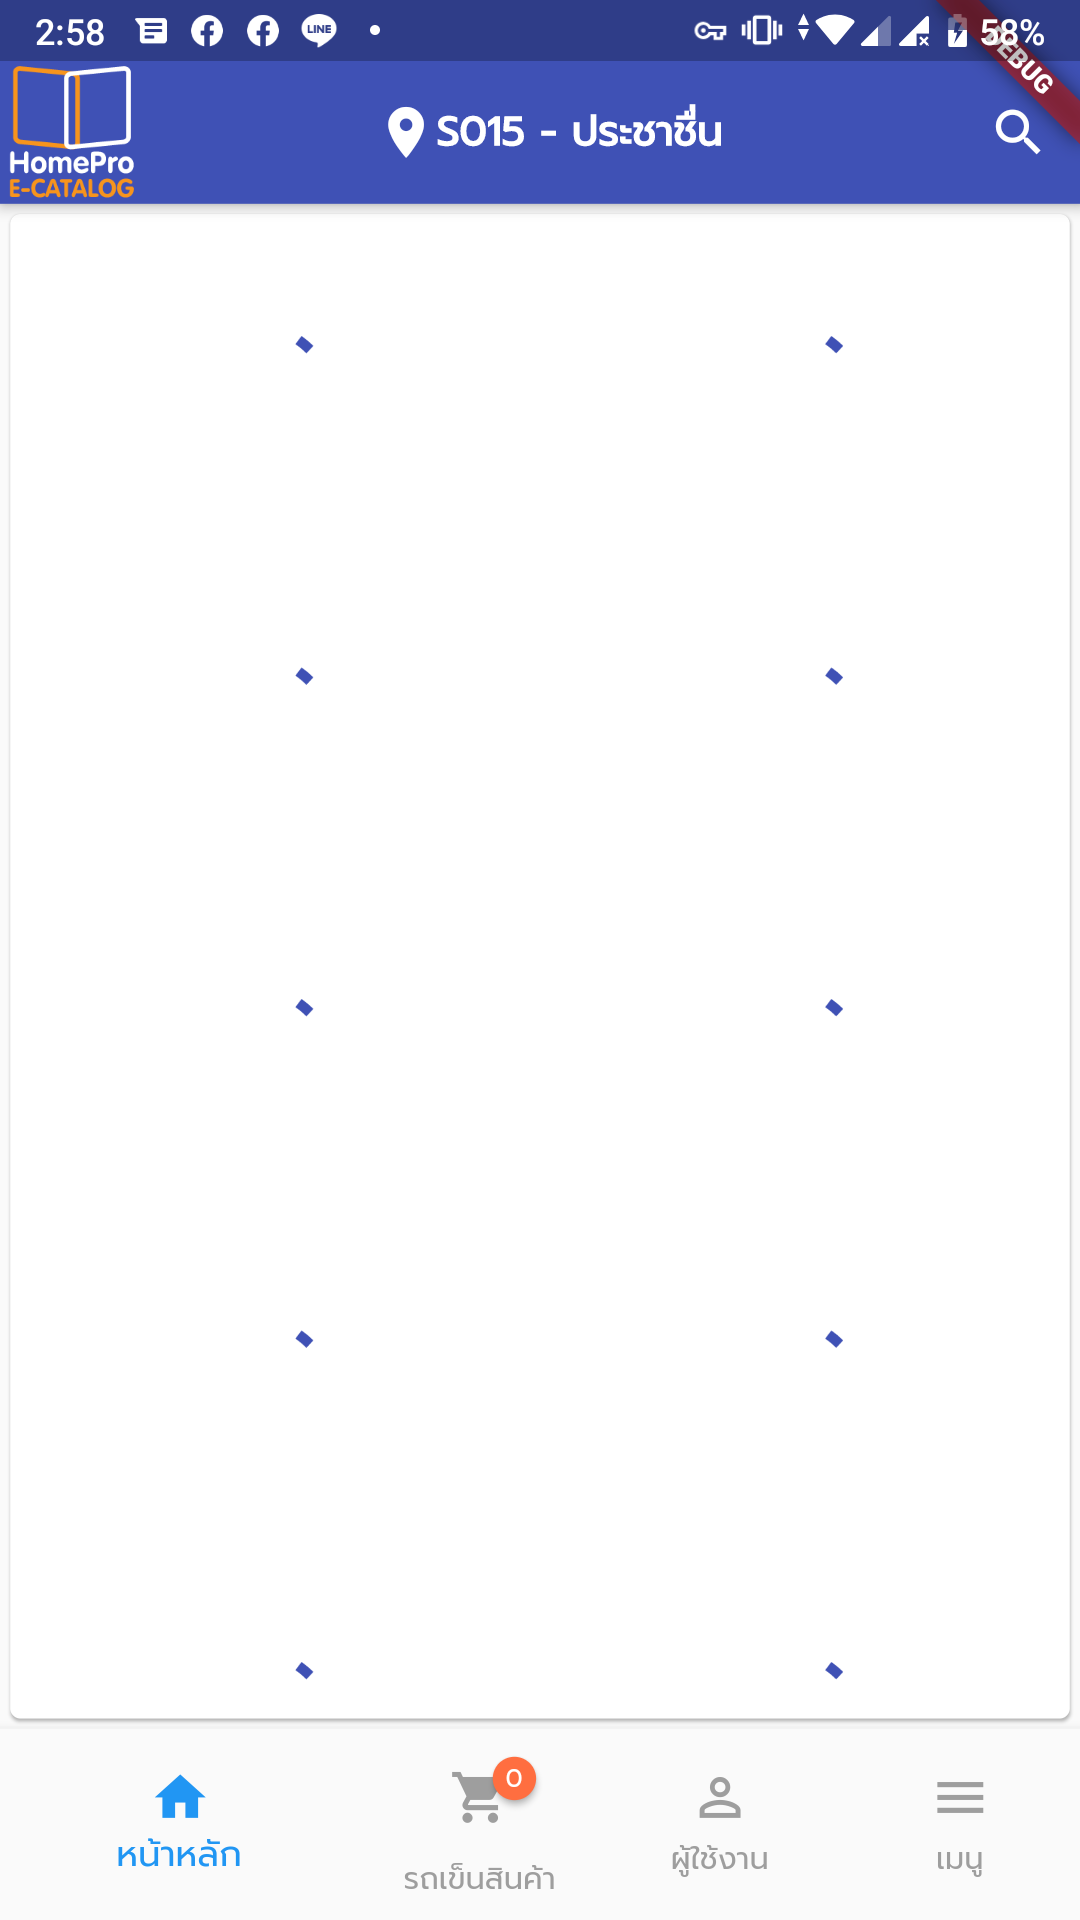
\includegraphics[width=0.35\textwidth]{1}
        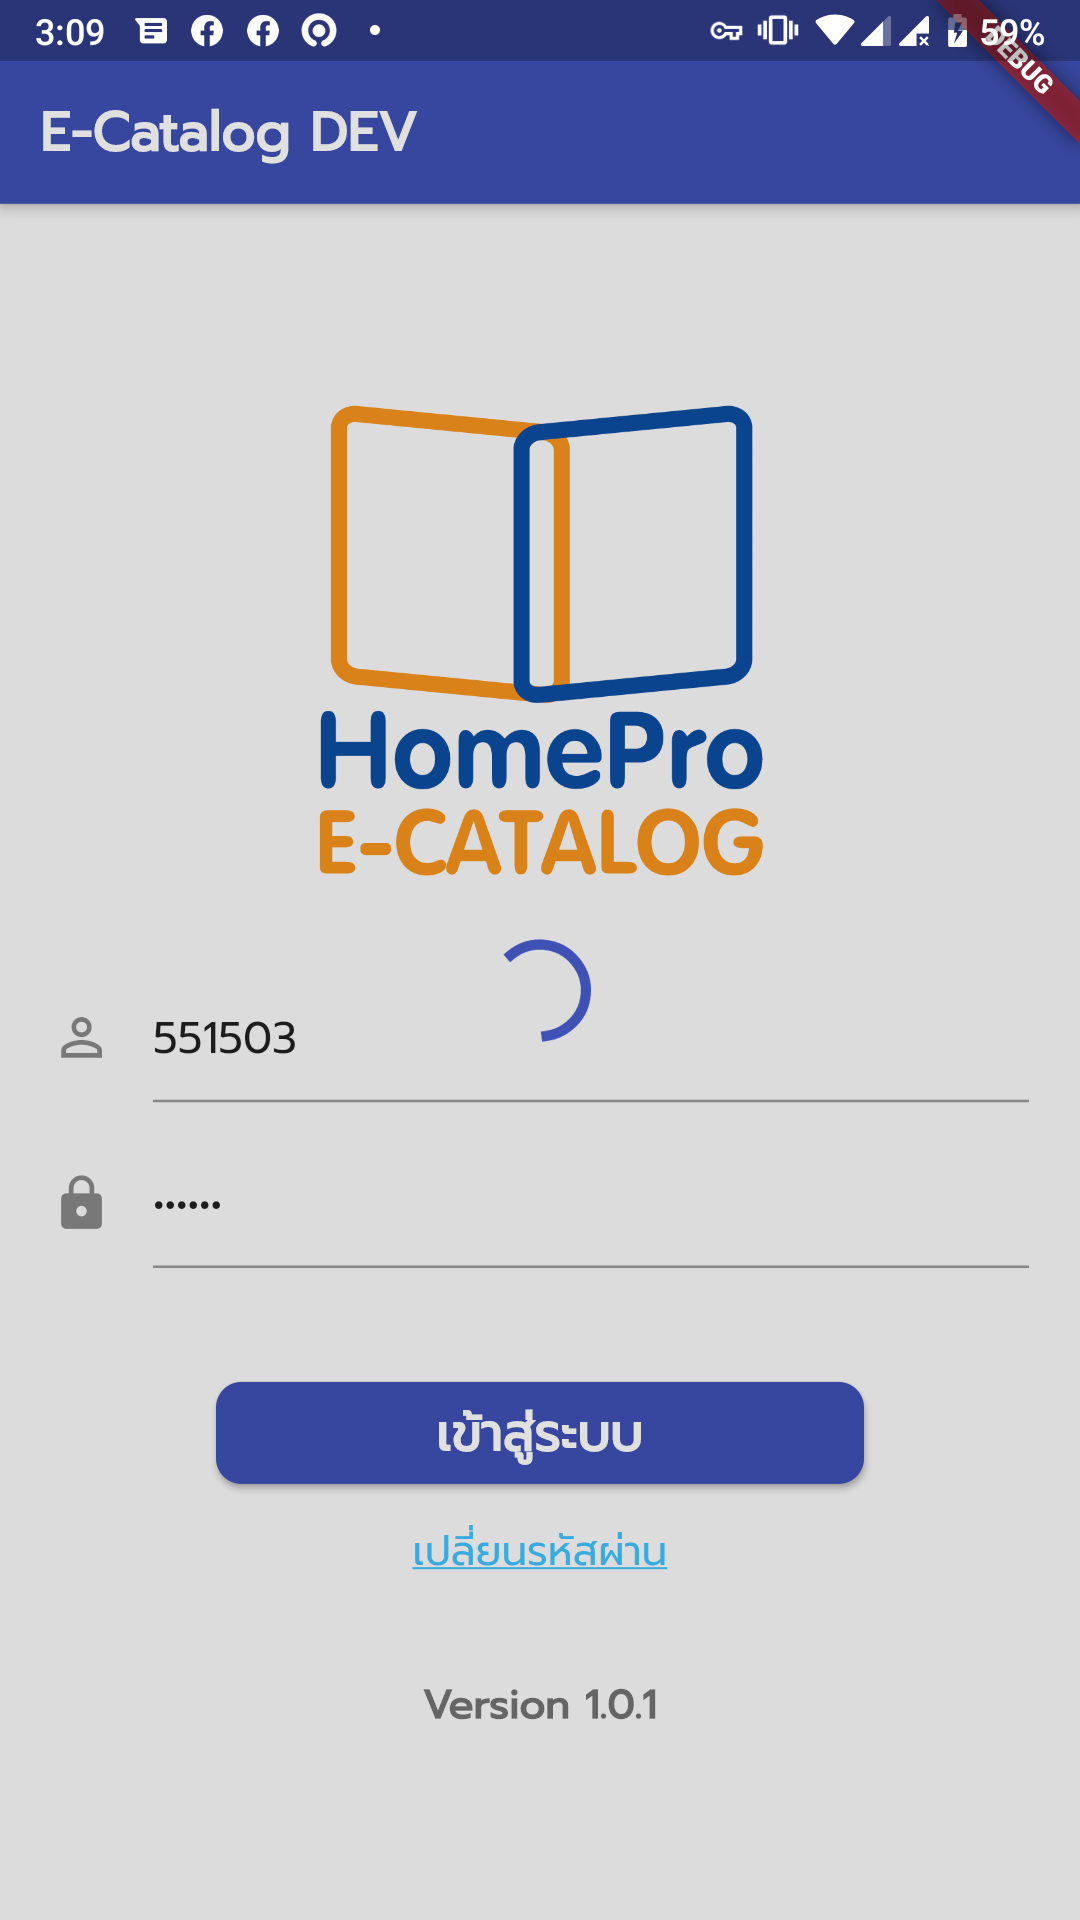
\includegraphics[width=0.35\textwidth]{2}
        \caption{ตัวอย่างการบันทึกหน้าจอเมื่อผิดผลาด}
        \label{errorPic}
    \end{figure}

    จากรูป 3.3 เป็นรูปที่เกิดจากการบันทึกหน้าจอเมื่อเจอข้อผิดผลาด (Test Fail) ดังตัวอย่างแสดงถึงเวลาที่หมดในการรอหน้าจอแสดงผลหรือใช้เวลาเกินกำหนดเป็นต้น

    \begin{longtable}{|l|l|}
        \caption{ตารางข้อเปรียบเทียบการทดสอบด้วยการจับ Element บนหน้าจอโดยไม่ต้องแก้ไขที่ Source Code}\\ 
        \hline
        \textbf{ข้อดี} & \textbf{ข้อเสีย} \endfirsthead 
        \hline
        \begin{tabular}[c]{@{}l@{}}สามารถจับ Element\\ได้โดยที่ไม่ต้อง\\ตามไปแก้ ที่ Source Code\end{tabular} & \begin{tabular}[c]{@{}l@{}}มีโอกาสที่ ลำดับของ \\Element \\จะคลาดเคลื่อน\\ตามขนาดโทรศัพท์\end{tabular}  \\ 
        \hline
        \begin{tabular}[c]{@{}l@{}}เปรียบเสมือนโทรศัพท์\\แสดงคีย์บอร์ดและกดได้\end{tabular}                   & \begin{tabular}[c]{@{}l@{}}บางคำสั่งอาจไม่รองรับการ\\ใช้งานกับ \\Appium ในคนละเวอร์ชัน\end{tabular}     \\
        \hline
    \end{longtable}

    \newpage
    \subsection{หน้า Log-in : กรอกรหัสพนักงาน และ รหัสผ่าน ถูกต้อง}
        \begin{longtable}{|l|l|l|} 
            \caption{ขอบเขตเหตุการณ์ Log-in ถูกต้อง} \\
            \hline
            \textbf{ลำดับ} & \textbf{เหตุการณ์ในการทดสอบ} & \textbf{ผลลัพธ์ในการทดสอบ}  \endfirsthead 
            \hline
            1              & กรอก username                & PASS                        \\ 
            \hline
            2              & กรอก password                & PASS                        \\ 
            \hline
            3              & กดปุ่ม login                 & PASS                        \\ 
            \hline
            4              & รอผลหน้าถัดไป                & PASS                        \\
            \hline
        \end{longtable}

        \begin{figure}[H]
            \centering
            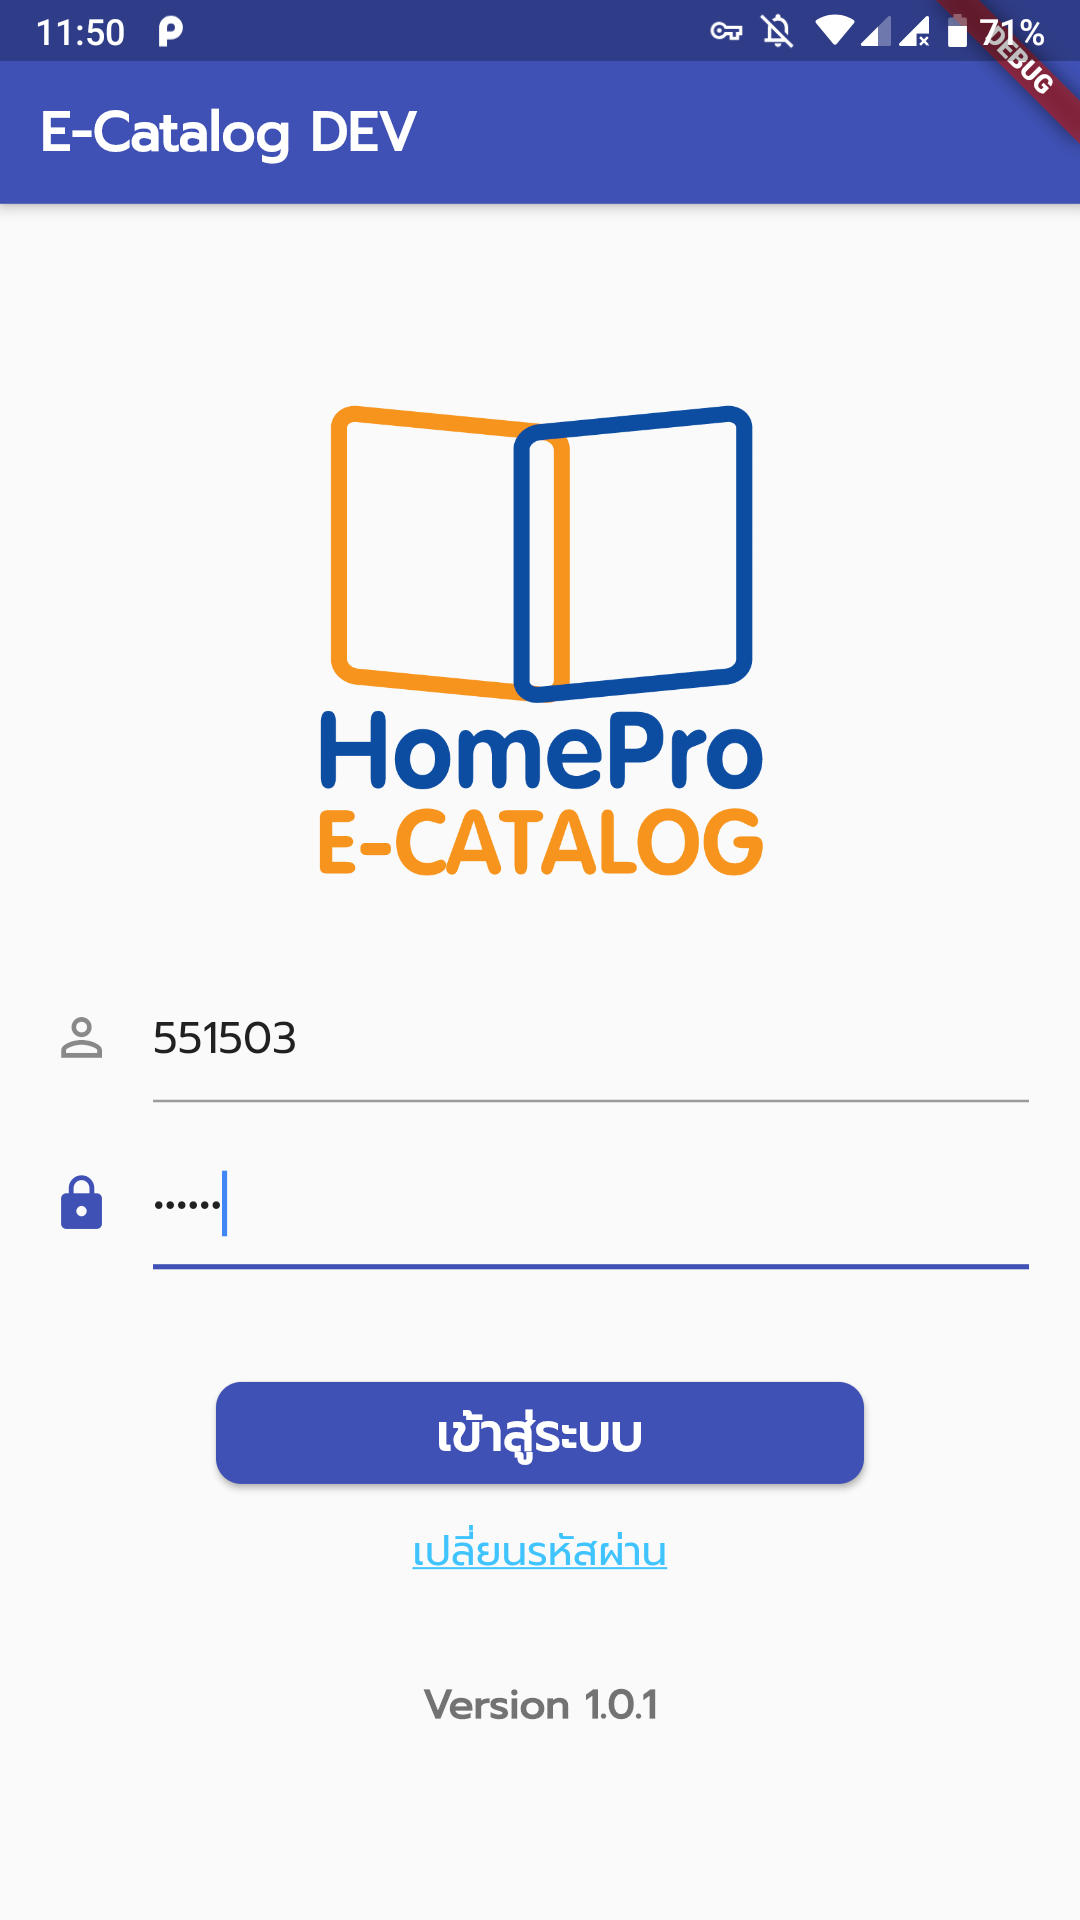
\includegraphics[width=0.35\textwidth]{loginPass2}
            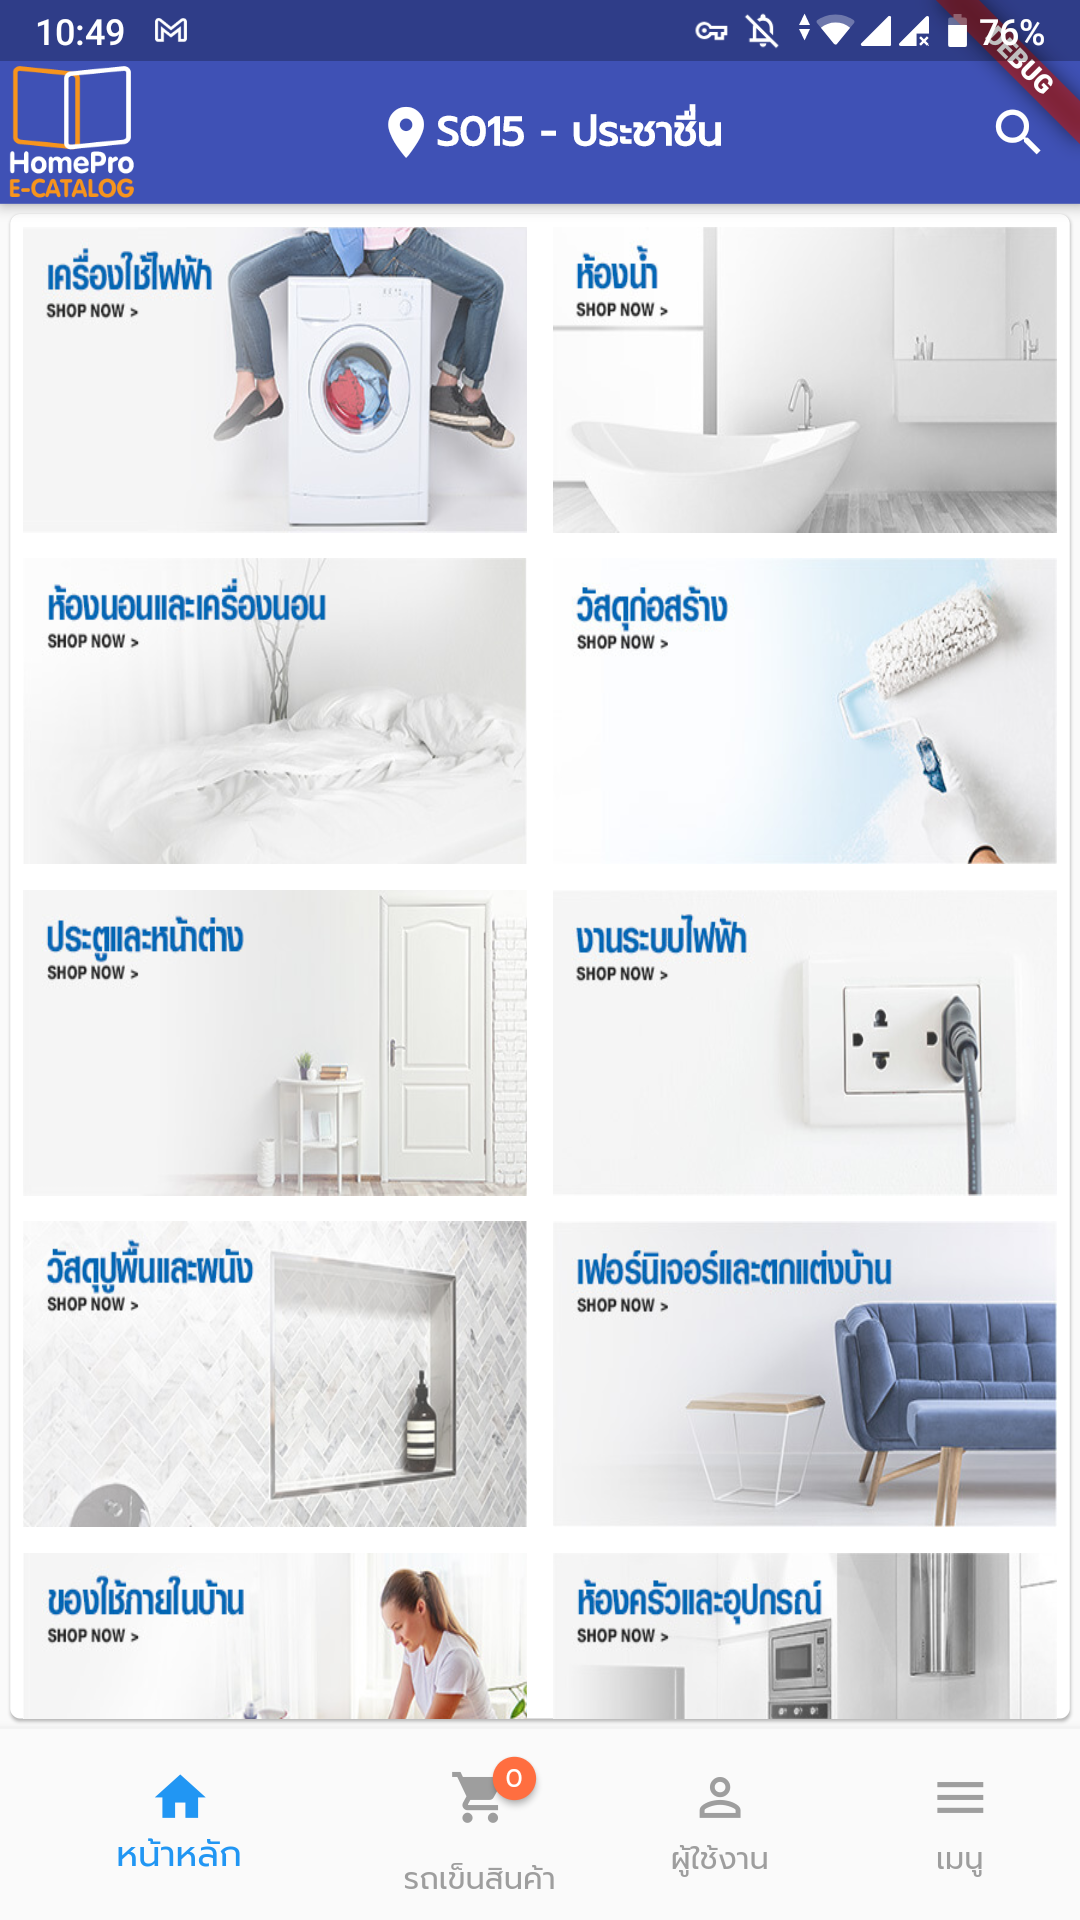
\includegraphics[width=0.35\textwidth]{loginPass3}
            \caption{ตัวอย่างเหตุการณ์ Log-in ถูกต้อง}
            \label{Fig:25}
        \end{figure}
    
    \newpage
    \subsection{หน้า Log-in : กรอกรหัสพนักงาน หรือ รหัสผ่าน ไม่ถูกต้อง}
        \begin{longtable}{|l|l|l|} 
            \caption{ขอบเขตเหตุการณ์ Log-in ไม่ถูกต้อง (กรอก usename ไม่ถูกต้อง)} \\
            \hline
            \textbf{ลำดับ} & \textbf{เหตุการณ์ในการทดสอบ} & \textbf{ผลลัพธ์ในการทดสอบ}  \endfirsthead 
            \hline
            1              & กรอก username ผิด               & PASS                        \\ 
            \hline
            2              & กรอก password                & PASS                        \\ 
            \hline
            3              & กดปุ่ม login                 & PASS                        \\ 
            \hline
            4              & ไม่พบข้อมูลผู้ใช้งาน                & PASS                        \\
            \hline
        \end{longtable}

        \begin{longtable}{|l|l|l|}
            \caption{ขอบเขตเหตุการณ์ Log-in ไม่ถูกต้อง (กรอก password ไม่ถูกต้อง)} \\ 
            \hline
            \textbf{ลำดับ} & \textbf{เหตุการณ์ในการทดสอบ} & \textbf{ผลลัพธ์ในการทดสอบ}  \endfirsthead 
            \hline
            1              & กรอก username               & PASS                        \\ 
            \hline
            2              & กรอก password ผิด                & PASS                        \\ 
            \hline
            3              & กดปุ่ม login                 & PASS                        \\ 
            \hline
            4              & รหัสผ่านไม่ถูกต้อง                & PASS                        \\
            \hline
        \end{longtable}

        \begin{figure}[H]
            \centering
            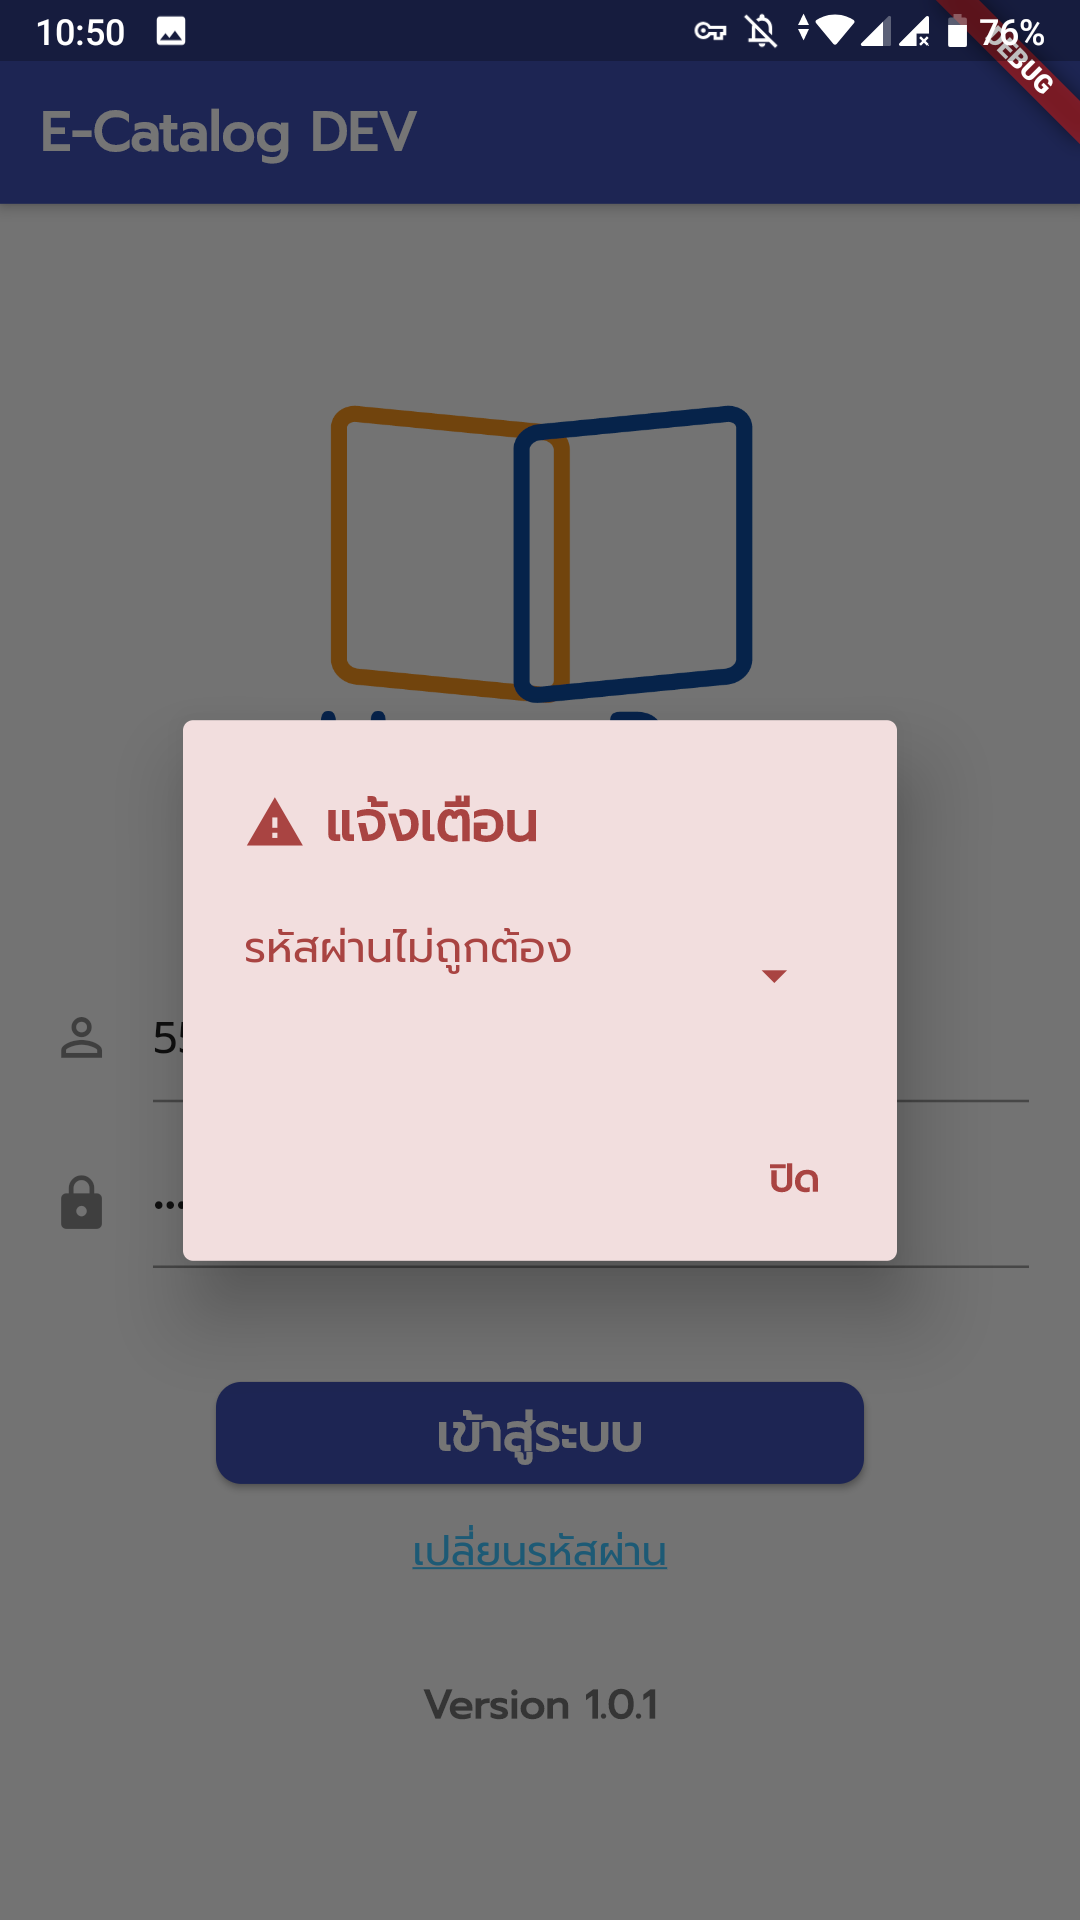
\includegraphics[width=0.35\textwidth]{loginFail1}
            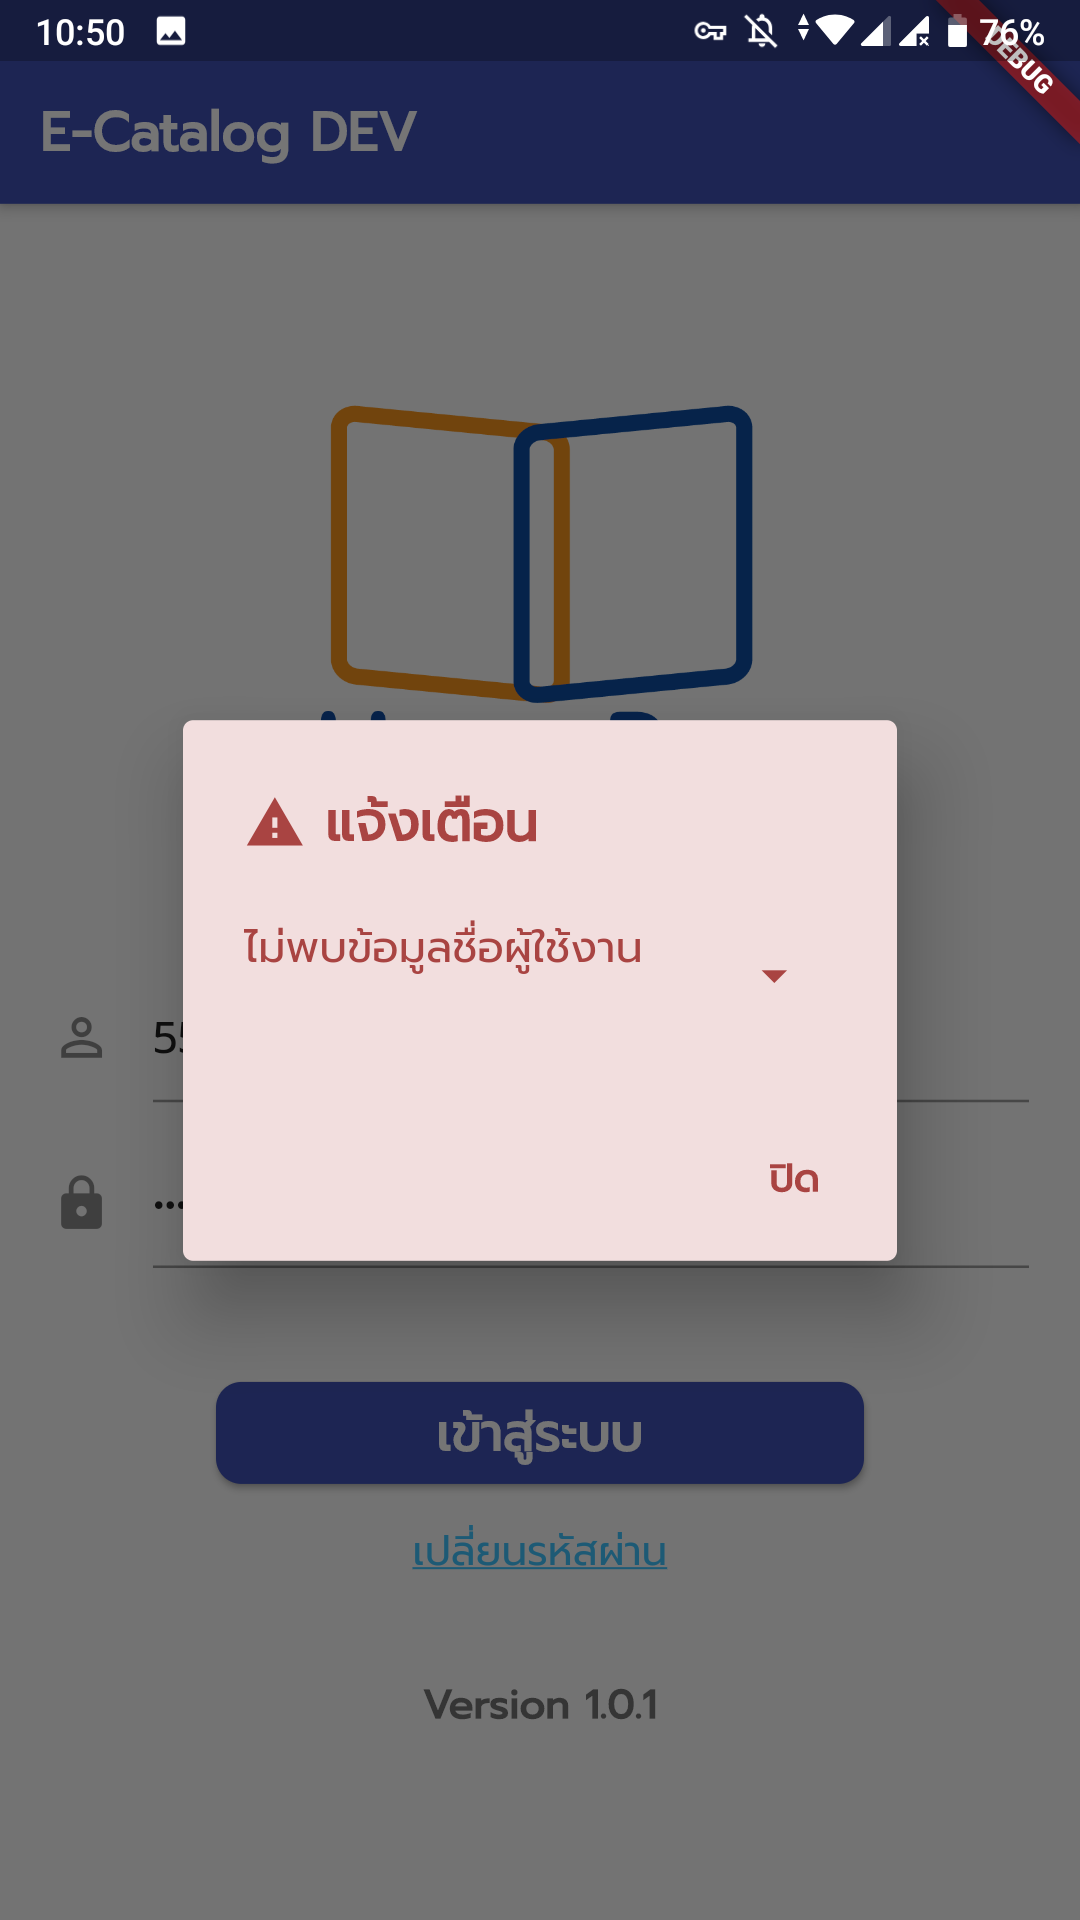
\includegraphics[width=0.35\textwidth]{loginFail2}
            \caption{ตัวอย่างเหตุการณ์ Log-in ถูกต้อง}
            \label{Fig:26}
        \end{figure}

    \newpage
    \subsection{ออกจากระบบ : ต้องการออกจากระบบด้วยแทบ "ผู้ใช้งาน" ใน BottomNavigationBar}

    \begin{longtable}{|l|l|l|}
        \caption{ขอบเขตเหตุการณ์ ออกจากระบบด้วยแทบ "ผู้ใช้งาน" ใน BottomNavigationBar} \\ 
        \hline
        \textbf{ลำดับ} & \textbf{เหตุการณ์ในการทดสอบ} & \textbf{ผลลัพธ์ในการทดสอบ}  \endfirsthead 
        \hline
        1              & ทำการ Log-in               & PASS                        \\ 
        \hline
        2              & กดไปที่ปุ่มผู้ใช้งาน                & PASS                        \\ 
        \hline
        3              & กดปุ่มออกจากระบบ                & PASS                        \\ 
        \hline
        4              & กดตกลงยืนยันและไปหน้า log-in     & PASS                        \\
        \hline
    \end{longtable}

    \begin{figure}[H]
        \centering
        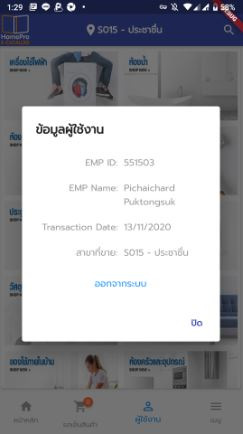
\includegraphics[width=0.35\textwidth]{logout1_2}
        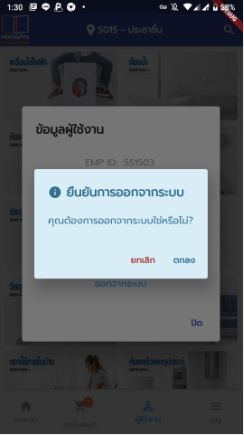
\includegraphics[width=0.35\textwidth]{logout1_3}
        \caption{ตัวอย่างเหตุการณ์ ออกจากระบบด้วยแทบ "ผู้ใช้งาน" ใน BottomNavigationBar}
        \label{Fig:27}
    \end{figure}

    \newpage
    \subsection{ออกจากระบบ : ต้องการออกจากระบบด้วยแทบ "เมนู" ใน BottomNavigationBar}

    \begin{longtable}{|l|l|l|} 
        \caption{ขอบเขตเหตุการณ์ ออกจากระบบด้วยแทบ "เมนู" ใน BottomNavigationBar} \\
        \hline
        \textbf{ลำดับ} & \textbf{เหตุการณ์ในการทดสอบ} & \textbf{ผลลัพธ์ในการทดสอบ}  \endfirsthead 
        \hline
        1              & ทำการ Log-in               & PASS                        \\ 
        \hline
        2              & กดไปที่ปุ่มเมนู               & PASS                        \\ 
        \hline
        3              & กดปุ่มออกจากระบบ                & PASS                        \\ 
        \hline
        4              & กดตกลงยืนยันและไปหน้า log-in     & PASS                        \\
        \hline
    \end{longtable}

    \begin{figure}[H]
        \centering
        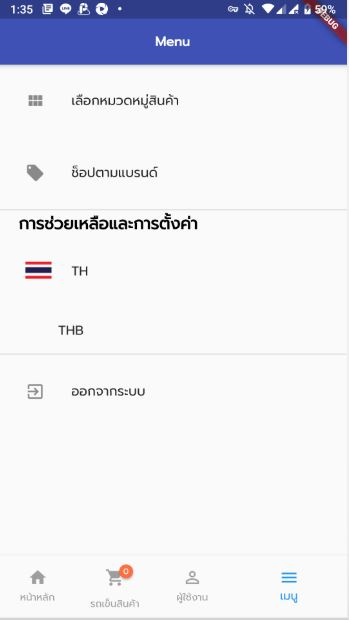
\includegraphics[width=0.35\textwidth]{logout2}
        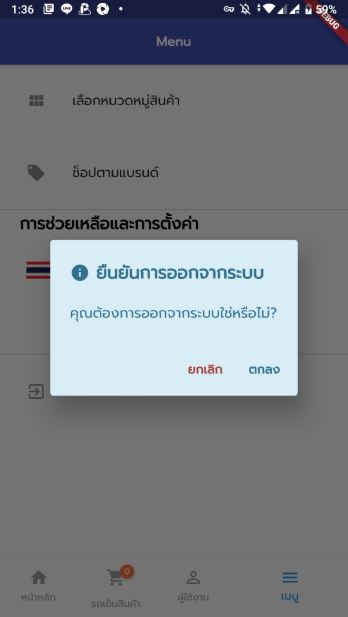
\includegraphics[width=0.35\textwidth]{logout2_1}
        \caption{ตัวอย่างเหตุการณ์ ออกจากระบบด้วยแทบ "เมนู" ใน BottomNavigationBar}
        \label{Fig:28}
    \end{figure}

    \newpage
    \subsection{หน้าหลัก - รายละเอียดสินค้า (Detail) : ตรวจสอบรายละเอียดของสินค้า}

    สามารถแบ่งได้เป็น 2 ประเภทคือ รายละเอียดสินค้า ราคาธรรมดาและสินค้าราคาโปรโมชัน

    \begin{longtable}{|l|l|l|}
        \caption{ขอบเขตเหตุการณ์ รายละเอียดสินค้า (Detail) ตรวจสอบรายละเอียดของสินค้าธรรมดา} \\ 
        \hline
        \textbf{ลำดับ} & \textbf{เหตุการณ์ในการทดสอบ} & \textbf{ผลลัพธ์ในการทดสอบ}  \endfirsthead 
        \hline
        1              & ทำการ Log-in               & PASS                        \\ 
        \hline
        2              & กดไปที่หมวดเครื่องใช้ไฟฟ้า               & PASS                        \\ 
        \hline
        3              & กดปุ่มหมวดย่อยไปที่เครื่องเตรียมอาหาร                & PASS                        \\ 
        \hline
        4              & เลือกสินค้าธรรมดา     & PASS                        \\
        \hline
        5              & เช็คแบรนสินค้า     & PASS                        \\
        \hline
        6              & เช็คชื่อสินค้า     & PASS                        \\
        \hline
        7              & เช็ครหัสสินค้า     & PASS                        \\
        \hline
        8              & เช็คราคาแบบธรรมดา     & PASS                        \\
        \hline
    \end{longtable}

    \begin{longtable}{|l|l|l|} 
        \caption{ขอบเขตเหตุการณ์ รายละเอียดสินค้า (Detail) ตรวจสอบรายละเอียดของสินค้ามีโปรโมชัน} \\
        \hline
        \textbf{ลำดับ} & \textbf{เหตุการณ์ในการทดสอบ} & \textbf{ผลลัพธ์ในการทดสอบ}  \endfirsthead 
        \hline
        1              & ทำการ Log-in               & PASS                        \\ 
        \hline
        2              & กดไปที่หมวดเครื่องใช้ไฟฟ้า               & PASS                        \\ 
        \hline
        3              & กดปุ่มหมวดย่อยไปที่เครื่องเตรียมอาหาร                & PASS                        \\ 
        \hline
        4              & เลือกสินค้าธรรมดา     & PASS                        \\
        \hline
        5              & เช็คแบรนสินค้า     & PASS                        \\
        \hline
        6              & เช็คชื่อสินค้า     & PASS                        \\
        \hline
        7              & เช็ครหัสสินค้า     & PASS                        \\
        \hline
        8              & เช็คราคาแบบธรรมดา     & PASS                        \\
        \hline
        9              & เช็คราคาแบบโปรโมชั่น     & PASS                        \\
        \hline
    \end{longtable}

    \begin{figure}[H]
        \centering
        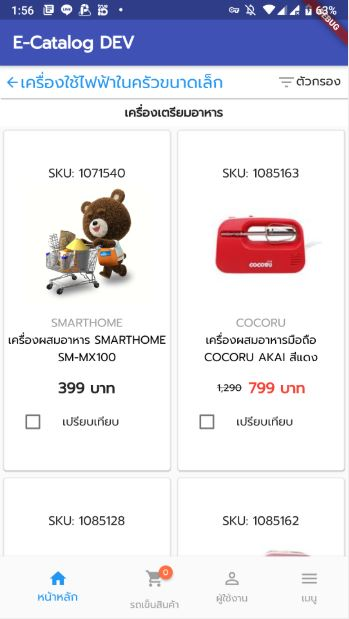
\includegraphics[width=0.35\textwidth]{detail1_2.JPG}
        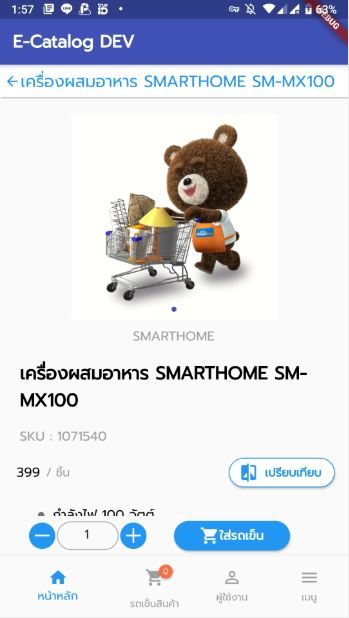
\includegraphics[width=0.35\textwidth]{detail1_3.JPG}
        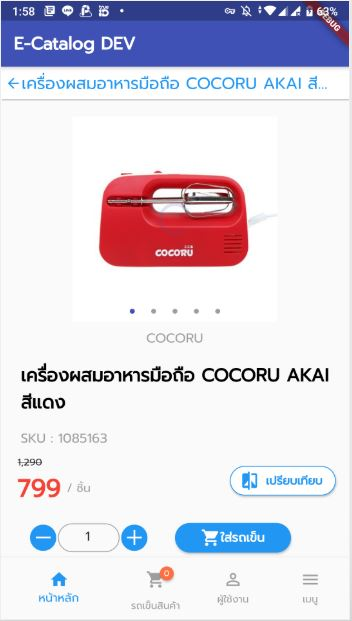
\includegraphics[width=0.35\textwidth]{detail1_4.JPG}
        \caption{ตัวอย่างเหตุการณ์ รายละเอียดสินค้า (Detail) ตรวจสอบรายละเอียดของสินค้า}
        \label{Fig:51}
    \end{figure}

    \newpage
    \subsection{หน้าหลัก - รายละเอียดสินค้า (Detail) : ปุ่มเปรียบเทียบ หน้า Detail}

    \begin{longtable}{|l|l|l|} 
        \caption{ขอบเขตเหตุการณ์ รายละเอียดสินค้า (Detail) ปุ่มเปรียบเทียบ หน้า Detail} \\
        \hline
        \textbf{ลำดับ} & \textbf{เหตุการณ์ในการทดสอบ} & \textbf{ผลลัพธ์ในการทดสอบ}  \endfirsthead 
        \hline
        1              & ทำการ Log-in               & PASS                        \\ 
        \hline
        2              & เลือกสินค้า               & PASS                        \\ 
        \hline
        3              & กดปุ่มเปรียบเทียบ                & PASS                        \\ 
        \hline
        4              & เช็คว่ามีสินค้าในช่องเปรียบเทียบ     & PASS                        \\
        \hline
    \end{longtable}

    \begin{figure}[H]
        \centering
        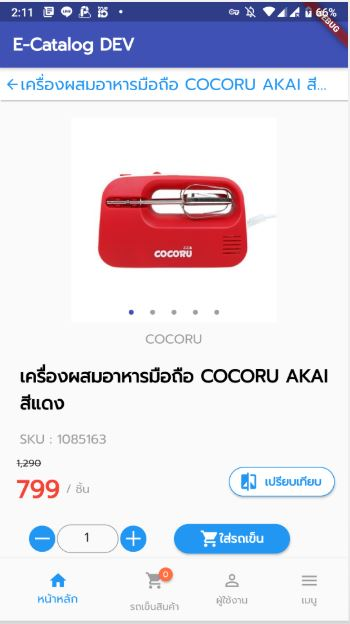
\includegraphics[width=0.35\textwidth]{detailCom1.JPG}
        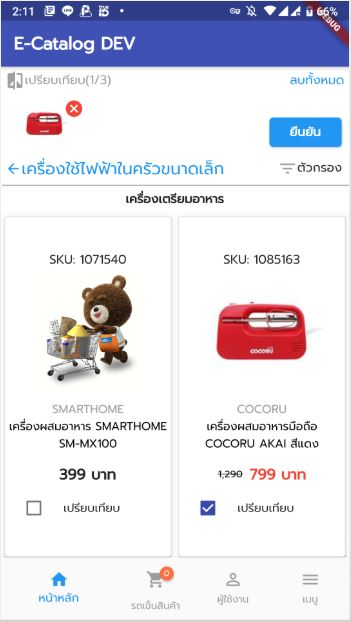
\includegraphics[width=0.35\textwidth]{deatilCom2.JPG}
        \caption{ตัวอย่างเหตุการณ์ รายละเอียดสินค้า (Detail) ปุ่มเปรียบเทียบ หน้า Detail}
        \label{Fig:59}
    \end{figure}


    \subsection{หน้าหลัก - รายละเอียดสินค้า (Detail) : แถบรายละเอียดสินค้า}

    \begin{longtable}{|l|l|l|}
        \caption{ขอบเขตเหตุการณ์ รายละเอียดสินค้า (Detail) แถบรายละเอียดสินค้า} \\ 
        \hline
        \textbf{ลำดับ} & \textbf{เหตุการณ์ในการทดสอบ} & \textbf{ผลลัพธ์ในการทดสอบ}  \endfirsthead 
        \hline
        1              & ทำการ Log-in               & PASS                        \\ 
        \hline
        2              & เลือกสินค้า               & PASS                        \\ 
        \hline
        3              & ไปหาเช็คแถบรายละเอียดสินค้ากดปุ่มเพิ่มเติม       & PASS                        \\ 
        \hline
        4              & มีรายละเอียดสินค้า     & PASS                        \\
        \hline
    \end{longtable}

    \begin{figure}[H]
        \centering
        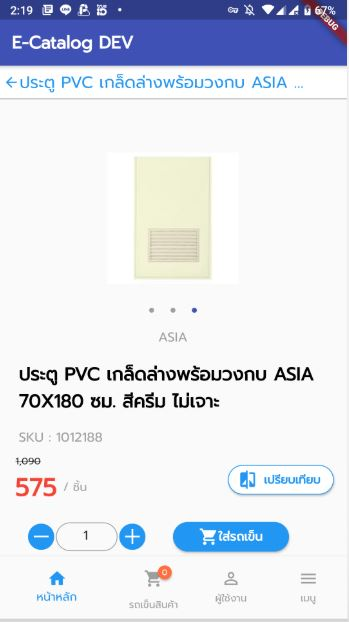
\includegraphics[width=0.35\textwidth]{deatilInfo1}
        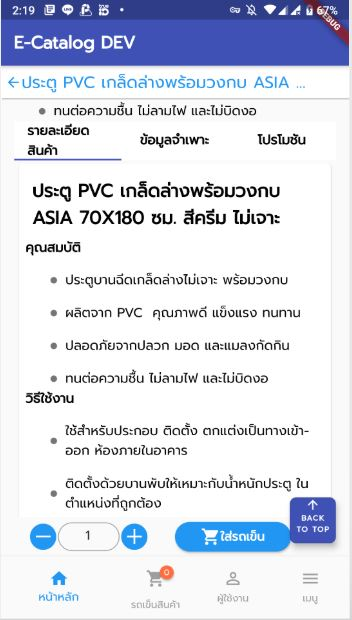
\includegraphics[width=0.35\textwidth]{detailInfo1_2}
        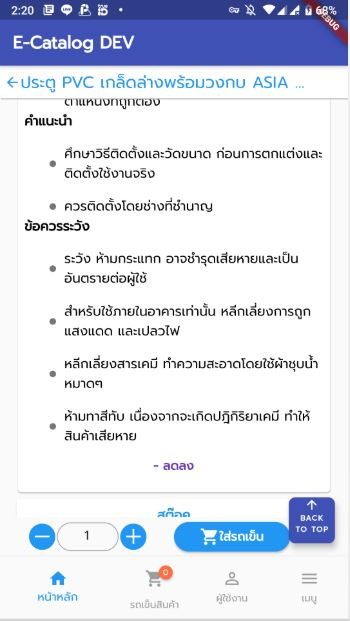
\includegraphics[width=0.35\textwidth]{detailInfo1_3}
        \caption{ตัวอย่างเหตุการณ์ รายละเอียดสินค้า (Detail) แถบรายละเอียดสินค้า}
        \label{Fig:29}
    \end{figure}

    \newpage
    \subsection{หน้าหลัก - รายละเอียดสินค้า (Detail) : แถบข้อมูลจำเพาะ}

    \begin{longtable}{|l|l|l|}
        \caption{ขอบเขตเหตุการณ์ รายละเอียดสินค้า (Detail) แถบข้อมูลจำเพาะ} \\ 
        \hline
        \textbf{ลำดับ} & \textbf{เหตุการณ์ในการทดสอบ} & \textbf{ผลลัพธ์ในการทดสอบ}  \endfirsthead 
        \hline
        1              & ทำการ Log-in               & PASS                        \\ 
        \hline
        2              & เลือกสินค้า               & PASS                        \\ 
        \hline
        3              & ไปยังหมวดข้อมูลจำเพาะ       & PASS                        \\ 
        \hline
        4              & เช็ค Brand     & PASS                        \\
        \hline
        5              & เช็ค Color     & PASS                        \\
        \hline
        6              & เช็ค ประเภทหน้าบาน     & PASS                        \\
        \hline
        7              & เช็ค ผิวเคลือบ     & PASS                        \\
        \hline
        8              & เช็ค การขึ้นรูป     & PASS                        \\
        \hline
        9              & เช็ค ลายหน้าบาน     & PASS                        \\
        \hline
        10              & เช็ค Material     & PASS                        \\
        \hline
        11             & เช็ค Size     & PASS                        \\
        \hline
    \end{longtable}

    \begin{figure}[H]
        \centering
        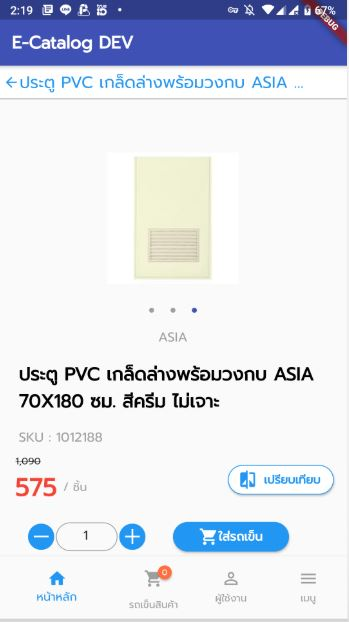
\includegraphics[width=0.35\textwidth]{deatilInfo1}
        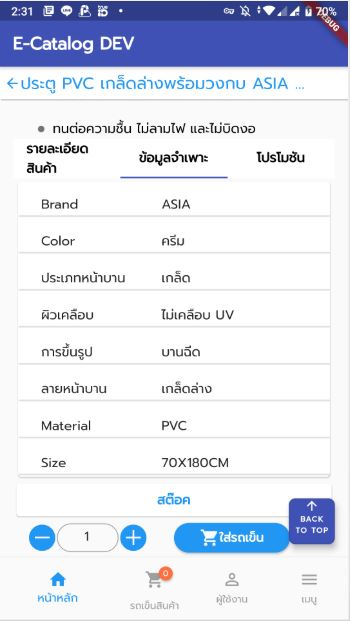
\includegraphics[width=0.35\textwidth]{detailInfo2.JPG}
        \caption{ตัวอย่างเหตุการณ์ รายละเอียดสินค้า (Detail) แถบข้อมูลจำเพาะ}
        \label{Fig:30}
    \end{figure}

    \newpage
    \subsection{หน้าหลัก - รายละเอียดสินค้า (Detail) : แถบโปรโมชั่นหน้าหลัก}

    \begin{longtable}{|l|l|l|} 
        \caption{ขอบเขตเหตุการณ์ รายละเอียดสินค้า (Detail) แถบโปรโมชั่นหน้าหลัก} \\
        \hline
        \textbf{ลำดับ} & \textbf{เหตุการณ์ในการทดสอบ} & \textbf{ผลลัพธ์ในการทดสอบ}  \endfirsthead 
        \hline
        1              & ทำการ Log-in               & PASS                        \\ 
        \hline
        2              & เลือกสินค้า               & PASS                        \\ 
        \hline
        3              & ไปยังหมวดโปรโมชัน       & PASS                        \\ 
        \hline
        4              & เช็ค โปรโมชัน 1 อันเป็นตัวอย่างว่าข้อมูลเข้า     & PASS                        \\
        \hline
    \end{longtable}

    \begin{figure}[H]
        \centering
        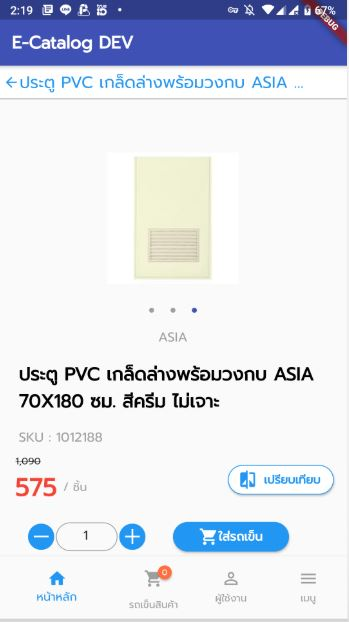
\includegraphics[width=0.35\textwidth]{deatilInfo1}
        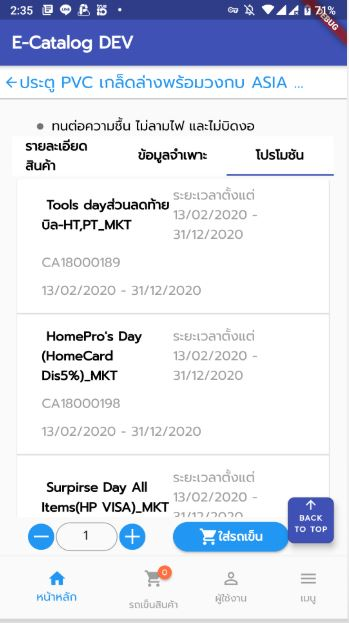
\includegraphics[width=0.35\textwidth]{detailPromotion}
        \caption{ตัวอย่างเหตุการณ์ รายละเอียดสินค้า (Detail) แถบโปรโมชั่นหน้าหลัก}
        \label{Fig:31}
    \end{figure}

    \newpage
    \subsection{หน้าหลัก - รายละเอียดสินค้า (Detail) : ปุ่ม สต๊อกสินค้า}

    \begin{longtable}{|l|l|l|} 
        \caption{ขอบเขตเหตุการณ์ รายละเอียดสินค้า (Detail) ปุ่ม สต๊อกสินค้า} \\
        \hline
        \textbf{ลำดับ} & \textbf{เหตุการณ์ในการทดสอบ} & \textbf{ผลลัพธ์ในการทดสอบ}  \endfirsthead 
        \hline
        1              & ทำการ Log-in               & PASS                        \\ 
        \hline
        2              & เลือกสินค้า               & PASS                        \\ 
        \hline
        3              & ไปหาและกดปุ่มสต๊อค       & PASS                        \\ 
        \hline
        4              & มีรายสาขาที่ของผู้ใช้ขึ้นก่อน     & PASS                        \\
        \hline
        5              & เป็นสาขา DC01     & PASS                        \\
        \hline
        6              & เป็นสาขา DC02     & PASS                        \\
        \hline
    \end{longtable}

    \begin{figure}[H]
        \centering
        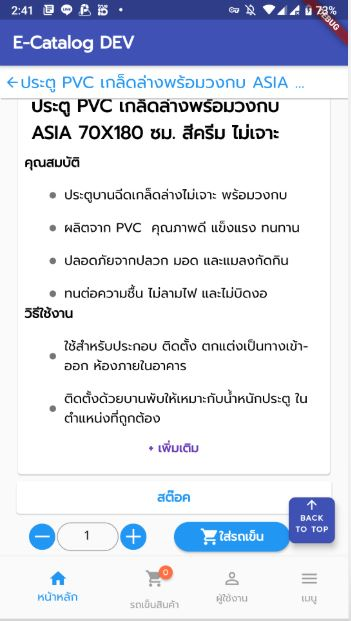
\includegraphics[width=0.35\textwidth]{stock1_2}
        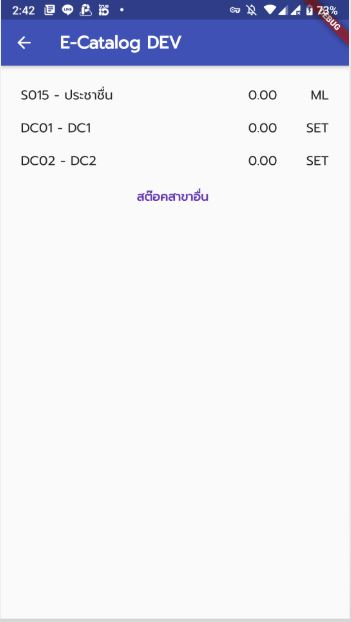
\includegraphics[width=0.35\textwidth]{stock1_3}
        \caption{ตัวอย่างเหตุการณ์ รายละเอียดสินค้า (Detail) ปุ่ม สต๊อกสินค้า}
        \label{Fig:32}
    \end{figure}

    \newpage
    \subsection{หน้าหลัก - รายละเอียดสินค้า (Detail) : ปุ่ม สต๊อกสินค้าเพิ่มเติม}

    \begin{longtable}{|l|l|l|} 
        \caption{ขอบเขตเหตุการณ์ รายละเอียดสินค้า (Detail) ปุ่ม สต๊อกสินค้าเพิ่มเติม} \\
        \hline
        \textbf{ลำดับ} & \textbf{เหตุการณ์ในการทดสอบ} & \textbf{ผลลัพธ์ในการทดสอบ}  \endfirsthead 
        \hline
        1              & ทำการ Log-in               & PASS                        \\ 
        \hline
        2              & เลือกสินค้า               & PASS                        \\ 
        \hline
        3              & ไปหาและกดปุ่มสต๊อค       & PASS                        \\ 
        \hline
        4              & กดไปที่สต๊อคสาขาอื่น     & PASS                        \\
        \hline
        5              & เช็คลำดับสต๊อคจากสาขามีมากไปน้อย     & PASS                        \\
        \hline
    \end{longtable}

    \begin{figure}[H]
        \centering
        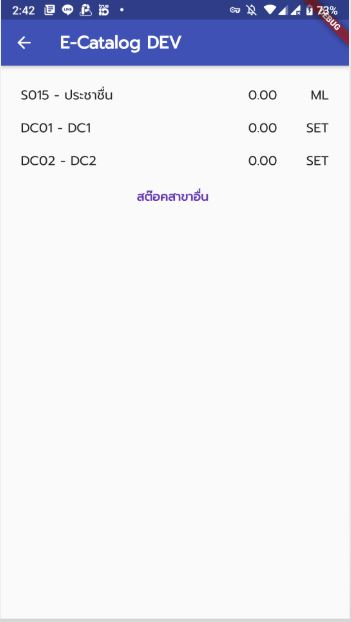
\includegraphics[width=0.35\textwidth]{stock1_3}
        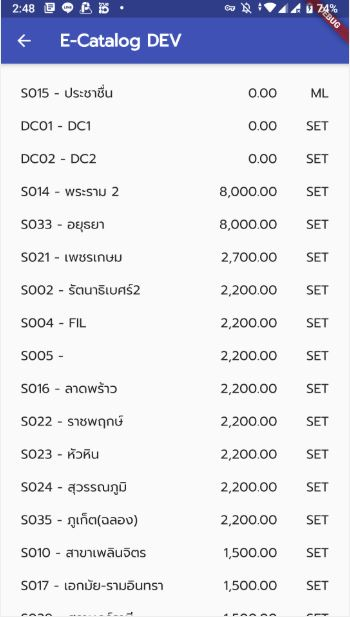
\includegraphics[width=0.35\textwidth]{stockMore.JPG}
        \caption{ตัวอย่างเหตุการณ์ รายละเอียดสินค้า (Detail) ปุ่ม สต๊อกสินค้าเพิ่มเติม}
        \label{Fig:33}
    \end{figure}

    \newpage
    \subsection{หน้าจอเปรียบเทียบสินค้า : เปรียบเทียบ}

    \begin{longtable}{|l|l|l|} 
        \caption{ขอบเขตเหตุการณ์ เปรียบเทียบสินค้า} \\
        \hline
        \textbf{ลำดับ} & \textbf{เหตุการณ์ในการทดสอบ} & \textbf{ผลลัพธ์ในการทดสอบ}  \endfirsthead 
        \hline
        1              & ทำการ Log-in               & PASS                        \\ 
        \hline
        2              & ไปยังหมวดหมู่ย่อย               & PASS                        \\ 
        \hline
        3              & กดเลือกปุ่มเปรียบเทียบสินค้า 3 ชิ้น       & PASS                        \\ 
        \hline
        4              & กดยืนยันการเปรียบเทียบ     & PASS                        \\
        \hline
        5              & เช็ค ความกว้าง     & PASS                        \\
        \hline
        6              & เช็ค ความลึก     & PASS                        \\
        \hline
        7              & เช็ค Material     & PASS                        \\
        \hline
        8              & เช็ค ระดับ     & PASS                        \\
        \hline
        9              & เช็ค อุปกรณ์เสริม     & PASS                        \\
        \hline
        10              & เช็ค ฺBrand     & PASS                        \\
        \hline
        11              & เช็ค ความสูง     & PASS                        \\
        \hline
        12              & เช็ค น้ำหนัก     & PASS                        \\
        \hline
        13              & เช็ค กำลังไฟ     & PASS                        \\
        \hline
        14              & เช็ค Size     & PASS                        \\
        \hline
        15              & เช็ค Color     & PASS                        \\
        \hline
    \end{longtable}

    \begin{figure}[H]
        \centering
        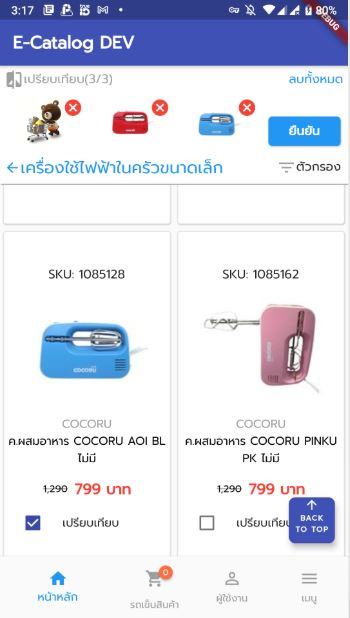
\includegraphics[width=0.35\textwidth]{compare1_2}
        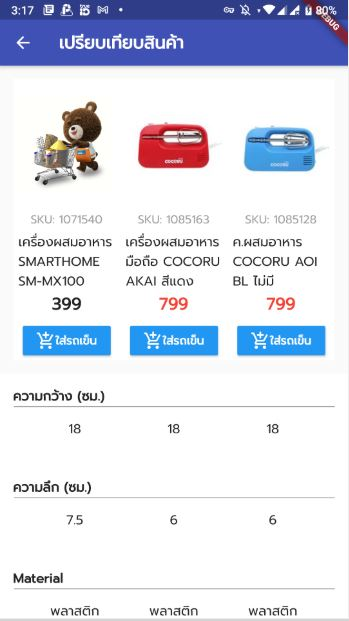
\includegraphics[width=0.35\textwidth]{compare1_3}
        \caption{ตัวอย่างเหตุการณ์ เปรียบเทียบสินค้า}
        \label{Fig:34}
    \end{figure}

    \newpage
    \subsection{หน้าจอเปรียบเทียบสินค้า : เปรียบเทียบมากกว่า 3 รายการ}

    \begin{longtable}{|l|l|l|} 
        \caption{ขอบเขตเหตุการณ์ เปรียบเทียบมากกว่า 3 รายการ} \\
        \hline
        \textbf{ลำดับ} & \textbf{เหตุการณ์ในการทดสอบ} & \textbf{ผลลัพธ์ในการทดสอบ}  \endfirsthead 
        \hline
        1              & ทำการ Log-in               & PASS                        \\ 
        \hline
        2              & ไปยังหมวดหมู่ย่อย               & PASS                        \\ 
        \hline
        3              & กดเลือกปุ่มเปรียบเทียบสินค้า 4 ชิ้น       & PASS                        \\ 
        \hline
        4              & แสดงจำนวนสินค้าเปรียบเทียบเกินกำหนด     & PASS                        \\
        \hline
    \end{longtable}

    \begin{figure}[H]
        \centering
        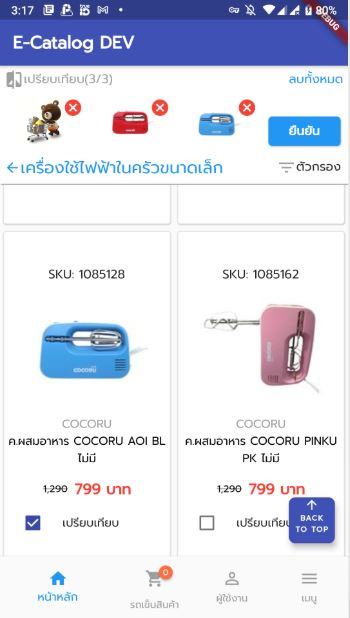
\includegraphics[width=0.35\textwidth]{compare1_2}
        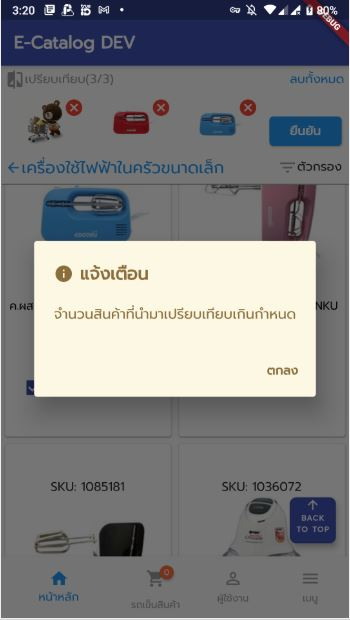
\includegraphics[width=0.35\textwidth]{compareMore}
        \caption{ตัวอย่างเหตุการณ์ เปรียบเทียบมากกว่า 3 รายการ}
        \label{Fig:35}
    \end{figure}

    \subsection{หน้าจอเปรียบเทียบสินค้า : ยกเลิกตัวที่เปรียบเทียบบางรายการ}

    \begin{longtable}{|l|l|l|}
        \caption{ขอบเขตเหตุการณ์ ยกเลิกตัวที่เปรียบเทียบบางรายการ} \\ 
        \hline
        \textbf{ลำดับ} & \textbf{เหตุการณ์ในการทดสอบ} & \textbf{ผลลัพธ์ในการทดสอบ}  \endfirsthead 
        \hline
        1              & ทำการ Log-in               & PASS                        \\ 
        \hline
        2              & ไปยังหมวดหมู่ย่อย               & PASS                        \\ 
        \hline
        3              & กดเลือกปุ่มเปรียบเทียบสินค้า 3 ชิ้น       & PASS                        \\ 
        \hline
        4              & กดปุ่มลบสินค้าต้องเหลือสินค้า 2 ชิ้น     & PASS                        \\
        \hline
    \end{longtable}

    \begin{figure}[H]
        \centering
        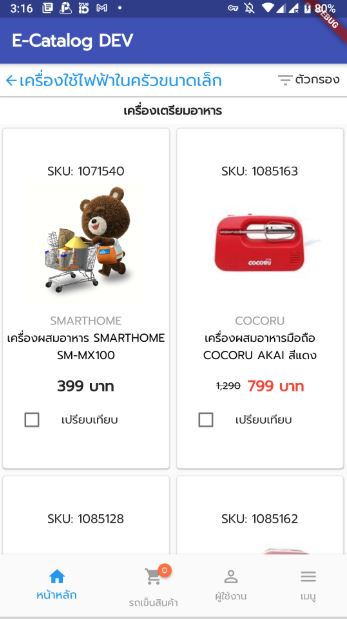
\includegraphics[width=0.35\textwidth]{compare1_1}
        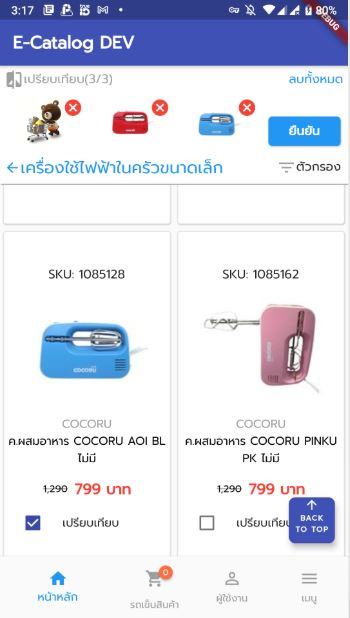
\includegraphics[width=0.35\textwidth]{compare1_2}
        \includegraphics[width=0.35\textwidth]{delsome}
        \caption{ตัวอย่างเหตุการณ์ ยกเลิกตัวที่เปรียบเทียบบางรายการ}
        \label{Fig:36}
    \end{figure}

    \newpage
    \subsection{หน้าจอเปรียบเทียบสินค้า :ยกเลิกการเปรียบเทียบทั้งหมด}

    \begin{longtable}{|l|l|l|}
        \caption{ขอบเขตเหตุการณ์ยกเลิกการเปรียบเทียบทั้งหมด} \\ 
        \hline
        \textbf{ลำดับ} & \textbf{เหตุการณ์ในการทดสอบ} & \textbf{ผลลัพธ์ในการทดสอบ}  \endfirsthead 
        \hline
        1              & ทำการ Log-in               & PASS                        \\ 
        \hline
        2              & ไปยังหมวดหมู่ย่อย               & PASS                        \\ 
        \hline
        3              & กดเลือกปุ่มเปรียบเทียบสินค้า 3 ชิ้น       & PASS                        \\ 
        \hline
        4              & กดปุ่มลบทั้งหมดช่องเปรียบเทียบหาย    & PASS                        \\
        \hline
    \end{longtable}

    \begin{figure}[H]
        \centering
        \includegraphics[width=0.35\textwidth]{compare1_2}
        \includegraphics[width=0.35\textwidth]{compare1_1}
        \caption{ตัวอย่างเหตุการณ์ยกเลิกการเปรียบเทียบทั้งหมด}
        \label{Fig:37}
    \end{figure}

    \subsection{หน้าจอเปรียบเทียบสินค้า : ปุ่ม เพิ่มลงรถเข็น}

    \begin{longtable}{|l|l|l|}
        \caption{ขอบเขตเหตุการณ์ ปุ่ม เพิ่มลงรถเข็น} \\ 
        \hline
        \textbf{ลำดับ} & \textbf{เหตุการณ์ในการทดสอบ} & \textbf{ผลลัพธ์ในการทดสอบ}  \endfirsthead 
        \hline
        1              & ทำการ Log-in               & PASS                        \\ 
        \hline
        2              & ไปยังหมวดหมู่ย่อย               & PASS                        \\ 
        \hline
        3              & กดเลือกปุ่มเปรียบเทียบสินค้า 3 ชิ้น       & PASS                        \\ 
        \hline
        4              & กดยืนยันการเปรียบเทียบ     & PASS                        \\
        \hline
        5              & กดปุ่มใส่รถเข็น     & PASS                        \\
        \hline
        6              & สินค้าไปอยู่ในแถบรถเข็นสินค้า     & PASS                        \\
        \hline
    \end{longtable}

    \begin{figure}[H]
        \centering
        \includegraphics[width=0.35\textwidth]{compare1_1}
        \includegraphics[width=0.35\textwidth]{compare1_2}
        \includegraphics[width=0.35\textwidth]{compare1_3}
        \includegraphics[width=0.35\textwidth]{compareCart}
        \caption{ตัวอย่างเหตุการณ์ ปุ่ม เพิ่มลงรถเข็น}
        \label{Fig:38}
    \end{figure}

    \subsection{รถเข็นสินค้า – แก้ไขรายการสินค้า : แก้ไขจำนวนสินค้า (เพิ่ม-ลด)}

    \begin{longtable}{|l|l|l|}
        \caption{ขอบเขตเหตุการณ์ รถเข็นสินค้า – แก้ไขรายการสินค้า แก้ไขจำนวนสินค้า (เพิ่ม-ลด)} \\ 
        \hline
        \textbf{ลำดับ} & \textbf{เหตุการณ์ในการทดสอบ} & \textbf{ผลลัพธ์ในการทดสอบ}  \endfirsthead 
        \hline
        1              & ทำการ Log-in               & PASS                        \\ 
        \hline
        2              & เลือกสินค้าใส่รถเข็น               & PASS                        \\ 
        \hline
        3              & ไปยังแถบ รถเข็นสินค้า       & PASS                        \\ 
        \hline
        4              & กดปุ่มเพิ่ม 2 ครั้ง     & PASS                        \\
        \hline
        5              & กดปุ่มลด 1 ครั้ง     & PASS                        \\
        \hline
        6              & เทียบจำนวนสินค้ากับเลขบนรูปรถเข็น     & PASS                        \\
        \hline
        7              & เทียบจำนวนสินค้ากับราคา     & PASS                        \\
        \hline
    \end{longtable}

    \begin{figure}[H]
        \centering
        \includegraphics[width=0.35\textwidth]{compareCart}
        \includegraphics[width=0.35\textwidth]{cart1_1.JPG}
        \includegraphics[width=0.35\textwidth]{cart1_2.JPG}
        \caption{ตัวอย่างเหตุการณ์ รถเข็นสินค้า – แก้ไขรายการสินค้า แก้ไขจำนวนสินค้า (เพิ่ม-ลด)}
        \label{Fig:39}
    \end{figure}

    \newpage
    \subsection{รถเข็นสินค้า – แก้ไขรายการสินค้า : แก้ไขจำนวนสินค้า (เพิ่ม) โดยให้มี QTY รวมกันเกิน 999}

    \begin{longtable}{|l|l|l|}
        \caption{ขอบเขตเหตุการณ์ รถเข็นสินค้า – แก้ไขรายการสินค้า แก้ไขจำนวนสินค้า (เพิ่ม) โดยให้มี QTY รวมกันเกิน 999} \\ 
        \hline
        \textbf{ลำดับ} & \textbf{เหตุการณ์ในการทดสอบ} & \textbf{ผลลัพธ์ในการทดสอบ}  \endfirsthead 
        \hline
        1              & ทำการ Log-in               & PASS                        \\ 
        \hline
        2              & เลือกสินค้าใส่รถเข็น 2 ชิ้น            & PASS                        \\ 
        \hline
        3              & ไปยังแถบ รถเข็นสินค้า       & PASS                        \\ 
        \hline
        4              & แก้จำนวนสินค้า 1 อันให้เกิน 999     & PASS                        \\
        \hline
        5              & ทียบจำนวนสินค้ากับเลขบนรูปรถเข็นว่าเป็น 999+ ไหม    & PASS                        \\
        \hline
        6              & เทียบจำนวนสินค้ากับราคาของ 999+ ชิ้น     & PASS                        \\
        \hline
    \end{longtable}

    \begin{figure}[H]
        \centering
        \includegraphics[width=0.35\textwidth]{cart2_1}
        \includegraphics[width=0.35\textwidth]{cart2_2}
        \caption{ตัวอย่างเหตุการณ์ รถเข็นสินค้า – แก้ไขรายการสินค้า แก้ไขจำนวนสินค้า (เพิ่ม) โดยให้มี QTY รวมกันเกิน 999}
        \label{Fig:40}
    \end{figure}

    \newpage
    \subsection{รถเข็นสินค้า – แก้ไขรายการสินค้า : ลบรายการสินค้า}

    \begin{longtable}{|l|l|l|} 
        \caption{ขอบเขตเหตุการณ์ รถเข็นสินค้า – แก้ไขรายการสินค้า ลบรายการสินค้า} \\
        \hline
        \textbf{ลำดับ} & \textbf{เหตุการณ์ในการทดสอบ} & \textbf{ผลลัพธ์ในการทดสอบ}  \endfirsthead 
        \hline
        1              & ทำการ Log-in               & PASS                        \\ 
        \hline
        2              & เลือกสินค้าใส่รถเข็น 2 ชิ้น            & PASS                        \\ 
        \hline
        3              & ไปยังแถบ รถเข็นสินค้า       & PASS                        \\ 
        \hline
        4              & แก้จำนวนสินค้า 1 อันให้เกิน 999     & PASS                        \\
        \hline
        5              & ลบสินค้า 1 ชิ้น    & PASS                        \\
        \hline
        6              & เทียบจำนวนสินค้ากับเลขบนรูปรถเข็นลดลงจากที่ลบหรือไม่     & PASS                        \\
        \hline
        7              & เทียบราคาสินค้าว่าลดลงหรือไม่     & PASS                        \\
        \hline
    \end{longtable}

    \begin{figure}[H]
        \centering
        \includegraphics[width=0.35\textwidth]{cart2_2}
        \includegraphics[width=0.35\textwidth]{delcart}
        \caption{ตัวอย่างเหตุการณ์ รถเข็นสินค้า – แก้ไขรายการสินค้า ลบรายการสินค้า}
        \label{Fig:42}
    \end{figure}

    \newpage
    \subsection{รถเข็นสินค้า – สร้างใบคำสั่งซื้อ : สร้างใบคำสั่งซื้อ โดยใช้เบอร์โทรที่ไม่ใช่เบอร์มือถือ}

    \begin{longtable}{|l|l|l|} 
        \caption{ขอบเขตเหตุการณ์ รถเข็นสินค้า – สร้างใบคำสั่งซื้อ สร้างใบคำสั่งซื้อ โดยใช้เบอร์โทรที่ไม่ใช่เบอร์มือถือ} \\
        \hline
        \textbf{ลำดับ} & \textbf{เหตุการณ์ในการทดสอบ} & \textbf{ผลลัพธ์ในการทดสอบ}  \endfirsthead 
        \hline
        1              & ทำการ Log-in               & PASS                        \\ 
        \hline
        2              & เลือกสินค้าใส่รถเข็น 1 ชิ้น            & PASS                        \\ 
        \hline
        3              & ไปยังแถบ รถเข็นสินค้า       & PASS                        \\ 
        \hline
        4              & กรอกเบอร์โทรศพท์บ้าน     & PASS                        \\
        \hline
        5              & แจ้งเตือนแสดงว่าไม่ผ่าน     & PASS                        \\
        \hline
    \end{longtable}

    \begin{figure}[H]
        \centering
        \includegraphics[width=0.35\textwidth]{order1_2}
        \includegraphics[width=0.35\textwidth]{order1_3}
        \caption{ตัวอย่างเหตุการณ์ รถเข็นสินค้า – สร้างใบคำสั่งซื้อ สร้างใบคำสั่งซื้อ โดยใช้เบอร์โทรที่ไม่ใช่เบอร์มือถือ}
        \label{Fig:43}
    \end{figure}

    \newpage
    \subsection{รถเข็นสินค้า – สร้างใบคำสั่งซื้อ : สร้างใบคำสั่งซื้อ โดยใช้เบอร์โทรที่เบอร์มือถือถูกต้อง}

    \begin{longtable}{|l|l|l|} 
        \caption{ขอบเขตเหตุการณ์ รถเข็นสินค้า – สร้างใบคำสั่งซื้อ สร้างใบคำสั่งซื้อ โดยใช้เบอร์โทรที่เบอร์มือถือถูกต้อง} \\
        \hline
        \textbf{ลำดับ} & \textbf{เหตุการณ์ในการทดสอบ} & \textbf{ผลลัพธ์ในการทดสอบ}  \endfirsthead 
        \hline
        1              & ทำการ Log-in               & PASS                        \\ 
        \hline
        2              & เลือกสินค้าใส่รถเข็น 1 ชิ้น            & PASS                        \\ 
        \hline
        3              & ไปยังแถบ รถเข็นสินค้า       & PASS                        \\ 
        \hline
        4              & กรอกเบอร์โทรศพท์มือถือ     & PASS                        \\
        \hline
        5              & แจ้งเตือนแสดงว่าผ่าน     & PASS                        \\
        \hline
    \end{longtable}

    \begin{figure}[H]
        \centering
        \includegraphics[width=0.35\textwidth]{order2_2}
        \includegraphics[width=0.35\textwidth]{order2_3}
        \caption{ตัวอย่างเหตุการณ์ รถเข็นสินค้า – สร้างใบคำสั่งซื้อ สร้างใบคำสั่งซื้อ โดยใช้เบอร์โทรที่เบอร์มือถือถูกต้อง}
        \label{Fig:44}
    \end{figure}

    \newpage
    \subsection{ผู้ใช้งาน : ข้อมูลผู้เข้าใช้งาน}

    \begin{longtable}{|l|l|l|} 
        \caption{ขอบเขตเหตุการณ์ ผู้ใช้งาน ข้อมูลผู้เข้าใช้งาน} \\
        \hline
        \textbf{ลำดับ} & \textbf{เหตุการณ์ในการทดสอบ} & \textbf{ผลลัพธ์ในการทดสอบ}  \endfirsthead 
        \hline
        1              & ทำการ Log-in               & PASS                        \\ 
        \hline
        2              & กดไปที่ปุ่มผู้ใช้งาน                & PASS                        \\ 
        \hline
        3              & เช็ค EMP ID                & PASS                        \\ 
        \hline
        4              & เช็ค EMP Name     & PASS                        \\
        \hline
        5              & เช็ค Transaction Date     & PASS                        \\
        \hline
        6              & เช็ค EMP สาขาที่ขาย     & PASS                        \\
        \hline
    \end{longtable}

    \begin{figure}[H]
        \centering
        \includegraphics[width=0.35\textwidth]{user1}
        \includegraphics[width=0.35\textwidth]{user1_2}
        \caption{ตัวอย่างเหตุการณ์ ผู้ใช้งาน ข้อมูลผู้เข้าใช้งาน}
        \label{Fig:45}
    \end{figure}

    % เกิด Error ตั้งแต่ตรงนี้

    \newpage
    \subsection{เมนู – เลือกหมวดสินค้า : การค้นหาสินค้าจากการเลือกหมวดสินค้า}

    \begin{longtable}{|l|l|l|} 
        \caption{ขอบเขตเหตุการณ์ เมนู – เลือกหมวดสินค้า การค้นหาสินค้าจากการเลือกหมวดสินค้า} \\
        \hline
        \textbf{ลำดับ} & \textbf{เหตุการณ์ในการทดสอบ} & \textbf{ผลลัพธ์ในการทดสอบ}  \endfirsthead 
        \hline
        1              & ทำการ Log-in               & PASS                        \\ 
        \hline
        2              & กดไปที่ปุ่มเมนู               & PASS                        \\ 
        \hline
        3              & กดไปเลือกหมวดสินค้า                & PASS                        \\ 
        \hline
        4              & เลือกหมวดเครื่องใช้ไฟฟ้า     & PASS                        \\
        \hline
        5              & เช็ค ว่ามีหลอดไฟที่เป็นเครื่องใช้ไฟฟ้าหรือไม่     & PASS                        \\
        \hline
    \end{longtable}

    \begin{figure}[H]
        \centering
        \includegraphics[width=0.35\textwidth]{logout2}
        \includegraphics[width=0.35\textwidth]{logout2_1}
        \caption{ตัวอย่างเหตุการณ์ เมนู – เลือกหมวดสินค้า การค้นหาสินค้าจากการเลือกหมวดสินค้า}
        \label{Fig:46}
    \end{figure}


    \newpage
    \subsection{เมนู – เลือกหมวดสินค้า : การค้นหาสินค้าจากการเลือกแบรนด์สินค้า}

    \begin{longtable}{|l|l|l|}
        \caption{ขอบเขตเหตุการณ์ เมนู – เลือกหมวดสินค้า การค้นหาสินค้าจากการเลือกแบรนด์สินค้า} \\
        \hline
        \textbf{ลำดับ} & \textbf{เหตุการณ์ในการทดสอบ} & \textbf{ผลลัพธ์ในการทดสอบ}  \endfirsthead 
        \hline
        1              & ทำการ Log-in               & PASS                        \\ 
        \hline
        2              & กดไปที่ปุ่มเมนู               & PASS                        \\ 
        \hline
        3              & กดไปเลือกแบรนสินค้า                & PASS                        \\ 
        \hline
        4              & เลือกแบรน ALLUSION     & PASS                        \\
        \hline
        5              & เช็คว่ามีแบรน ALLUSION     & PASS                        \\
        \hline
    \end{longtable}

    \begin{figure}[H]
        \centering
        \includegraphics[width=0.35\textwidth]{brand1_1.JPG}
        \includegraphics[width=0.35\textwidth]{brand1_2.JPG}
        \caption{ตัวอย่างเหตุการณ์ เมนู – เลือกหมวดสินค้า การค้นหาสินค้าจากการเลือกแบรนด์สินค้า}
        \label{Fig:47}
    \end{figure}

    \newpage
    \subsection{เมนู – ภาษา : การเลือกภาษา}

    \begin{longtable}{|l|l|l|}
        \caption{ขอบเขตเหตุการณ์ เมนู – ภาษา การเลือกภาษา} \\
        \hline
        \textbf{ลำดับ} & \textbf{เหตุการณ์ในการทดสอบ} & \textbf{ผลลัพธ์ในการทดสอบ}  \endfirsthead 
        \hline
        1              & ทำการ Log-in               & PASS                        \\ 
        \hline
        2              & กดไปที่ปุ่มเมนู               & PASS                        \\ 
        \hline
        3              & กดไปเลือกที่เปลี่ยนภาษา                & PASS                        \\ 
        \hline
        4              & เลือกภาษาอังกฤษ     & PASS                        \\
        \hline
        5              & เช็คตัวภาษาด้านบนเปลี่ยนหรือไม่     & PASS                        \\
        \hline
    \end{longtable}

    \begin{figure}[H]
        \centering
        \includegraphics[width=0.35\textwidth]{lang1}
        \includegraphics[width=0.35\textwidth]{lang2}
        \caption{ตัวอย่างเหตุการณ์ เมนู – ภาษา การเลือกภาษา}
        \label{Fig:48}
    \end{figure}

    \subsection{หน้าหลัก - หมวดหมู่หลัก (Level 3) : ปุ่มค้นหา}
    วิธีนี้เลือกใช้การใช้กับ Driver Wd เนื่องจากต้องให้อุปกรณ์แสดงคีย์บอร์ดในการพิมพ์เพื่อ submit การค้นหาด้วย PressKeycode
    \begin{longtable}{|l|l|l|}
        \caption{ขอบเขตเหตุการณ์ หมวดหมู่หลัก (Level 3) ปุ่มค้นหา} \\
        \hline
        \textbf{ลำดับ} & \textbf{เหตุการณ์ในการทดสอบ} & \textbf{ผลลัพธ์ในการทดสอบ}  \endfirsthead 
        \hline
        1              & ทำการ Log-in               & PASS                        \\ 
        \hline
        2              & กดปุ่มและค้นหาสินค้า               & PASS                        \\ 
        \hline
        3              & แสดงสินค้ารหัส 255255               & PASS                        \\ 
        \hline
    \end{longtable}

    \begin{figure}[H]
        \centering
        \includegraphics[width=0.35\textwidth]{search}
        \includegraphics[width=0.35\textwidth]{search2}
        \caption{ตัวอย่างเหตุการณ์ หมวดหมู่หลัก (Level 3) ปุ่มค้นหา}
        \label{Fig:60}
    \end{figure}

\section{ผลการทดสอบด้วยการจับ แก้ไขที่ Source Code ของ Flutter โดยใช้ Appium Flutter Driver}
เป็นวิธีการทดสอบโดยการจับ Element กับแอปพลิเคชันที่ถูกสร้างด้วย Flutter ซึ่งต้องแก้ไขตัว Source Code ของแอปพลิเคชันโดยการใส่ Key ใน Element ที่จะจับดังตัวอย่างด้านล่าง 
\begin{figure}[H]
    \centering
    \includegraphics[width=1\textwidth]{keyAdd}
    \caption{ตัวอย่างการเพิ่ม Key กับ Element}\label{keyAdd}
\end{figure}

จากรูปที่ 3.30 เป็นการเพิ่ม Key ใน Element ของปุ่มซึ่งสามารถนำมาเรียกใช้ในการจับได้แต่ก็มีข้อจำกัดในบาง Element เช่น SlideBar เป็นต้นเนื่องจากจะจับตัวลากไม่ได้เลือก
 ใช้วิธีนี้เมื่อลำดับของ Element เปลี่ยนทำให้แบบไม่แก้ Source Code ไม่แน่นอน

\begin{figure}[H]
    \centering
    \includegraphics[width=1\textwidth]{resultFlutter}
    \includegraphics[width=1\textwidth]{resultFail}
    \caption{ตัวอย่างการแสดงผลการทดสอบแบบผ่านและมีข้อผิดพลาด}\label{keyAdd1}
\end{figure}

จากรูป 3.31 เป็นตัวอย่างการทดสอบหากผ่านการทดสอบและหากพบข้อผิดพลาดจะแสดงผลอย่างไร

\begin{longtable}{|l|l|}
    \caption{ตารางข้อเปรียบเทียบการทดสอบด้วยการจับ แก้ไขที่ Source Code ของ Flutter โดยใช้ Appium Flutter Driver}\\ 
    \hline
    \textbf{ข้อดี}  & \textbf{ข้อเสีย} \endfirsthead 
    \hline
    \begin{tabular}[c]{@{}l@{}}สามารถจับ Element ได้แม่นยำตาม\\key ที่ developer สร้างเอาไว้\end{tabular}                                                                      & \begin{tabular}[c]{@{}l@{}}ไม่สามารถแสดงคีย์บอร์ดที่เปรียบเสมือน\\การพิมพ์ได้ทำให้ไม่สามารถทดสอบบาง\\~function ได้\end{tabular}  \\ 
    \hline
    \begin{tabular}[c]{@{}l@{}}สามารถใช้ Flutter\_Driver ที่เป็นตัวทดสอบ\\~แอปพลิเคชันที่สร้างด้วย Flutter ที่ปกติเขียนด้วย \\Dart สามารถนำมาเขียนเป็นภาษาอื่นได้\end{tabular} & \begin{tabular}[c]{@{}l@{}}ต้องไปแก้ที่ Source Code และ \\build ใหม่เสมอเมื่อต้องการนำมาทดสอบ\end{tabular}                       \\ 
    \hline
                                                                                                                                                                               & \begin{tabular}[c]{@{}l@{}}ยังไม่สามารถนำ Flutter\_Driver \\มาใช้ได้อย่างสมบูรณ์เพราะพัฒนาไม่เสร็จ\end{tabular}                  \\
    \hline
\end{longtable}

    \newpage
    \subsection{หน้าหลัก - หมวดหมู่หลัก (Level 3) : ตรวจสอบการแสดงหมวดหมู่สินค้า}
    \begin{longtable}{|l|l|l|}
        \caption{ขอบเขตเหตุการณ์ หมวดหมู่หลัก (Level 3) ตรวจสอบการแสดงหมวดหมู่สินค้า} \\
        \hline
        \textbf{ลำดับ} & \textbf{เหตุการณ์ในการทดสอบ} & \textbf{ผลลัพธ์ในการทดสอบ}  \endfirsthead 
        \hline
        1              & ทำการ Log-in               & PASS                        \\ 
        \hline
        2              & เช็คชื่อหมวดทั้ง 16 หมวด               & PASS                        \\ 
        \hline
    \end{longtable}

    \begin{figure}[H]
        \centering
        \includegraphics[width=0.35\textwidth]{level3_1}
        \includegraphics[width=0.35\textwidth]{level3_2}
        \caption{ตัวอย่างเหตุการณ์ หมวดหมู่หลัก (Level 3) ตรวจสอบการแสดงหมวดหมู่สินค้า}
        \label{Fig:75}
    \end{figure}

    \newpage
    \subsection{หน้าหลัก - หมวดหมู่ย่อย (Level 2) : ตรวจสอบการแสดงหมวดหมู่สินค้า}
    \begin{longtable}{|l|l|l|}
        \caption{ขอบเขตเหตุการณ์ หมวดหมู่ย่อย (Level 2) ตรวจสอบการแสดงหมวดหมู่สินค้า} \\
        \hline
        \textbf{ลำดับ} & \textbf{เหตุการณ์ในการทดสอบ} & \textbf{ผลลัพธ์ในการทดสอบ}  \endfirsthead 
        \hline
        1              & ทำการ Log-in               & PASS                        \\ 
        \hline
        2              & กดเข้าทีละหมวด (level 3)             & PASS                        \\ 
        \hline
        3              & เช็คชื่อหมวดย่อย (level 2)               & PASS                        \\ 
        \hline
    \end{longtable}

    \begin{figure}[H]
        \centering
        \includegraphics[width=0.35\textwidth]{level2_1_1}
        \includegraphics[width=0.35\textwidth]{level2_1_2}
        \includegraphics[width=0.35\textwidth]{level2_1_3}
        \caption{ตัวอย่างเหตุการณ์ หมวดหมู่ย่อย (Level 2) ตรวจสอบการแสดงหมวดหมู่สินค้า}
        \label{Fig:61}
    \end{figure}

    \newpage
    \subsection{หน้าหลัก - หมวดหมู่ย่อย (Level 2) : ดูทั้งหมด}
    \begin{longtable}{|l|l|l|}
        \caption{ขอบเขตเหตุการณ์ หมวดหมู่ย่อย (Level 2) ดูทั้งหมด} \\
        \hline
        \textbf{ลำดับ} & \textbf{เหตุการณ์ในการทดสอบ} & \textbf{ผลลัพธ์ในการทดสอบ}  \endfirsthead 
        \hline
        1              & ทำการ Log-in               & PASS                        \\ 
        \hline
        2              & กดเข้าทีละหมวด (level 3)             & PASS                        \\ 
        \hline
        3              & กดปุ่มดูทั้งหมด (level 2)               & PASS                        \\ 
        \hline
        4              & เช็คการแสดงผลว่าตรงกับหมวดที่กดไหม (level 2)               & PASS                        \\ 
        \hline
    \end{longtable}

    \begin{figure}[H]
        \centering
        \includegraphics[width=0.35\textwidth]{level2_2_1}
        \includegraphics[width=0.35\textwidth]{level2_2_2}
        \caption{ตัวอย่างเหตุการณ์ หมวดหมู่ย่อย (Level 2) ดูทั้งหมด}
        \label{Fig:62}
    \end{figure}

    \newpage
    \subsection{หน้าหลัก - หมวดหมู่ย่อย (Level 1) : เลือกตัวกรอง – ตัวกรองหมวดสินค้า}
    \begin{longtable}{|l|l|l|}
        \caption{ขอบเขตเหตุการณ์ หมวดหมู่ย่อย (Level 1) เลือกตัวกรอง – ตัวกรองหมวดสินค้า} \\
        \hline
        \textbf{ลำดับ} & \textbf{เหตุการณ์ในการทดสอบ} & \textbf{ผลลัพธ์ในการทดสอบ}  \endfirsthead 
        \hline
        1              & ทำการ Log-in               & PASS                        \\ 
        \hline
        2              & กดเข้าหมวดกีฬา             & PASS                        \\ 
        \hline
        3              & กดปุ่มดูทั้งหมด (level 2)               & PASS                        \\ 
        \hline
        4              & กดสัญลักษณ์ปุ่ม filter               & PASS                        \\ 
        \hline
        5              & เลือกหมวดสินค้า              & PASS                        \\ 
        \hline
        6              & เช็คสินค้าว่าตรงกับหมวด              & PASS                        \\ 
        \hline
    \end{longtable}

    \begin{figure}[H]
        \centering
        \includegraphics[width=0.35\textwidth]{level1_1_2}
        \includegraphics[width=0.35\textwidth]{level1_1_3}
        \caption{ตัวอย่างเหตุการณ์ หมวดหมู่ย่อย (Level 1) เลือกตัวกรอง – ตัวกรองหมวดสินค้า}
        \label{Fig:70}
    \end{figure}

    \newpage
    \subsection{หน้าหลัก - หมวดหมู่ย่อย (Level 1) : เลือกตัวกรอง – ตัวกรองแบรนด์}
    \begin{longtable}{|l|l|l|}
        \caption{ขอบเขตเหตุการณ์ หมวดหมู่ย่อย (Level 1) เลือกตัวกรอง – ตัวกรองแบรนด์} \\
        \hline
        \textbf{ลำดับ} & \textbf{เหตุการณ์ในการทดสอบ} & \textbf{ผลลัพธ์ในการทดสอบ}  \endfirsthead 
        \hline
        1              & ทำการ Log-in               & PASS                        \\ 
        \hline
        2              & กดเข้าหมวดกีฬา             & PASS                        \\ 
        \hline
        3              & กดปุ่มดูทั้งหมด (level 2)               & PASS                        \\ 
        \hline
        4              & กดสัญลักษณ์ปุ่ม filter               & PASS                        \\ 
        \hline
        5              & เลือกแบรนด์              & PASS                        \\ 
        \hline
        6              & เช็คสินค้าว่าตรงกับแบรนด์ที่เลือก              & PASS                        \\ 
        \hline
    \end{longtable}

    \begin{figure}[H]
        \centering
        \includegraphics[width=0.35\textwidth]{level1_2_2}
        \includegraphics[width=0.35\textwidth]{level1_2_3}
        \caption{ตัวอย่างเหตุการณ์ หมวดหมู่ย่อย (Level 1) เลือกตัวกรอง – ตัวกรองแบรนด์}
        \label{Fig:63}
    \end{figure}

    \newpage
    \subsection{หน้าหลัก - หมวดหมู่ย่อย (Level 1) : ตรวจสอบการแสดงหมวดหมู่สินค้า Default}
    \begin{longtable}{|l|l|l|}
        \caption{ขอบเขตเหตุการณ์ หมวดหมู่ย่อย (Level 1) ตรวจสอบการแสดงหมวดหมู่สินค้า Default} \\
        \hline
        \textbf{ลำดับ} & \textbf{เหตุการณ์ในการทดสอบ} & \textbf{ผลลัพธ์ในการทดสอบ}  \endfirsthead 
        \hline
        1              & ทำการ Log-in               & PASS                        \\ 
        \hline
        2              & กดเข้าหมวดกีฬา             & PASS                        \\ 
        \hline
        3              & กดปุ่มดูทั้งหมด (level 2)               & PASS                        \\ 
        \hline
        4              & เช็คสินค้าว่าเรียงราคาจากน้อยไปมากตาม Default              & PASS                        \\ 
        \hline
    \end{longtable}

    \begin{figure}[H]
        \centering
        \includegraphics[width=0.35\textwidth]{level1_1_1}
        \includegraphics[width=0.35\textwidth]{level1_default}
        \caption{ตัวอย่างเหตุการณ์ หมวดหมู่ย่อย (Level 1) ตรวจสอบการแสดงหมวดหมู่สินค้า Default}
        \label{Fig:64}
    \end{figure}

    \newpage
    \subsection{หน้าหลัก - หมวดหมู่ย่อย (Level 1) : ตัวเลือก จัดเรียง – เรียงจากราคาน้อยไปหามาก}
    \begin{longtable}{|l|l|l|}
        \caption{ขอบเขตเหตุการณ์ หมวดหมู่ย่อย (Level 1) ตัวเลือก จัดเรียง – เรียงจากราคาน้อยไปหามาก} \\
        \hline
        \textbf{ลำดับ} & \textbf{เหตุการณ์ในการทดสอบ} & \textbf{ผลลัพธ์ในการทดสอบ}  \endfirsthead 
        \hline
        1              & ทำการ Log-in               & PASS                        \\ 
        \hline
        2              & กดเข้าหมวดกีฬา             & PASS                        \\ 
        \hline
        3              & กดปุ่มดูทั้งหมด (level 2)               & PASS                        \\ 
        \hline
        4              & กดสัญลักษณ์ปุ่ม filter               & PASS                        \\ 
        \hline
        5              & กดที่แถบเรียงตาม              & PASS                        \\ 
        \hline
        6              & เลือกราคาน้อยไปมาก              & PASS                        \\ 
        \hline
        7              & เช็คสินค้าเรียงราคาน้อยไปหามาก              & PASS                        \\ 
        \hline
    \end{longtable}

    \begin{figure}[H]
        \centering
        \includegraphics[width=0.35\textwidth]{level_less}
        \includegraphics[width=0.35\textwidth]{level_less2}
        \caption{ตัวอย่างเหตุการณ์ หมวดหมู่ย่อย (Level 1) ตัวเลือก จัดเรียง – เรียงจากราคาน้อยไปหามาก}
        \label{Fig:65}
    \end{figure}

    \newpage
    \subsection{หน้าหลัก - หมวดหมู่ย่อย (Level 1) : ตัวเลือก จัดเรียง – เรียงจากราคามากไปหาน้อย}
    \begin{longtable}{|l|l|l|}
        \caption{ขอบเขตเหตุการณ์ หมวดหมู่ย่อย (Level 1) ตัวเลือก จัดเรียง – เรียงจากราคามากไปหาน้อย} \\
        \hline
        \textbf{ลำดับ} & \textbf{เหตุการณ์ในการทดสอบ} & \textbf{ผลลัพธ์ในการทดสอบ}  \endfirsthead 
        \hline
        \textbf{ลำดับ} & \textbf{เหตุการณ์ในการทดสอบ} & \textbf{ผลลัพธ์ในการทดสอบ}  \endfirsthead 
        \hline
        1              & ทำการ Log-in               & PASS                        \\ 
        \hline
        2              & กดเข้าหมวดกีฬา             & PASS                        \\ 
        \hline
        3              & กดปุ่มดูทั้งหมด (level 2)               & PASS                        \\ 
        \hline
        4              & กดสัญลักษณ์ปุ่ม filter               & PASS                        \\ 
        \hline
        5              & กดที่แถบเรียงตาม              & PASS                        \\ 
        \hline
        6              & เลือกราคามากไปน้อย              & PASS                        \\ 
        \hline
        7              & เช็คสินค้าเรียงราคามากไปหาน้อย              & PASS                        \\ 
        \hline
    \end{longtable}

    \begin{figure}[H]
        \centering
        \includegraphics[width=0.35\textwidth]{level_more1}
        \includegraphics[width=0.35\textwidth]{level_more2}
        \caption{ตัวอย่างเหตุการณ์ หมวดหมู่ย่อย (Level 1) ตัวเลือก จัดเรียง – เรียงจากราคามากไปหาน้อย}
        \label{Fig:66}
    \end{figure}

    \newpage
    \subsection{หน้าหลัก - หมวดหมู่ย่อย (Level 1) : ตัวเลือก เปรียบสินค้าหน้าหลัก}
    \begin{longtable}{|l|l|l|}
        \caption{ขอบเขตเหตุการณ์ หมวดหมู่ย่อย (Level 1) ตัวเลือก เปรียบสินค้าหน้าหลัก} \\
        \hline
        \textbf{ลำดับ} & \textbf{เหตุการณ์ในการทดสอบ} & \textbf{ผลลัพธ์ในการทดสอบ}  \endfirsthead 
        \hline
        \textbf{ลำดับ} & \textbf{เหตุการณ์ในการทดสอบ} & \textbf{ผลลัพธ์ในการทดสอบ}  \endfirsthead 
        \hline
        1              & ทำการ Log-in               & PASS                        \\ 
        \hline
        2              & กดเข้าหมวดกีฬา             & PASS                        \\ 
        \hline
        3              & กดปุ่มดูทั้งหมด (level 2)               & PASS                        \\ 
        \hline
        4              & กดปุ่มเปรียบเทียบ 2 อัน             & PASS                        \\ 
        \hline
        5              & สินค้า 2 ชิ้นอยู่แถบเปรียบเทียบ              & PASS                        \\ 
        \hline
    \end{longtable}

    \begin{figure}[H]
        \centering
        \includegraphics[width=0.35\textwidth]{level1_1_1}
        \includegraphics[width=0.35\textwidth]{level1_compare}
        \caption{ตัวอย่างเหตุการณ์ หมวดหมู่ย่อย (Level 1) ตัวเลือก เปรียบสินค้าหน้าหลัก}
        \label{Fig:67}
    \end{figure}

\newpage
\section{ข้อจำกัดของการทดสอบในโครงการด้วย AWS Device Farm}
การใช้ AWS Device Farm ใช้เพื่อลดเวลาในการทดสอบและความหลากหลายของอุปกรณ์ในการทดสอบ

\begin{figure}[H]
    \centering
    \includegraphics[width=1\textwidth]{devicefram1}
    \includegraphics[width=1\textwidth]{devicefarm2}
    \caption{ตัวอย่างผลการทดลองนำไปทดสอบบน AWS Device Farm}
    \label{Fig:90}
\end{figure}

จากรูป 3.42 ค้นพบว่าการทดสอบบน AWS Device Farm กับแอปพลิเคชัน HomePro E-Catalog ไม่สามารถทำได้เพราะแอปพลิเคชันนี้รองรับในการใช้กับอินเทอร์เน็ตภายในองค์กรเท่านั้น


\begin{figure}[H]
    \centering
    \includegraphics[width=0.5\textwidth]{test1}
    \caption{ตัวอย่างภาพบันทึกหน้าจอจาก AWS Devices Farm}
    \label{Fig:90}
\end{figure}

จากรูป 3.42 คือรูปที่เกิดจากการบันทึกหน้าจอจาก AWS Device Farm ตอนทำการทดสอบและแสดงว่าไม่สามารถทดสอบได้

\subsection{แนวทางการแก้ปัญหา}
การแก้ปัญหาคือการที่จะต้องสร้าง Amazon Virtual Private Cloud ซึ่งจะต้องมีค่าใช้จ่ายในการทำเพื่อที่จะสามารถเชื่อมต่อกับอินเทอร์เน็ตภายในองค์กรได้แต่ทางองค์กรไม่ได้จัดสรรส่วนนี้ให้ในการทำการทดสอบทำให้ไม่สามารถนำ ชุดคำสั่งทดสอบ แอปพลิเคชัน HomePro E-Catalog ไปทดสอบบน AWS Devices Farm ได้

\newpage
\section{สรุปการทดลองทั้งหมดของ HomePro E-Catalog}
\begin{longtable}{|l|l|} 
    \caption{ตารางผลการทดสอบเหตุการณ์ทั้งหมด 35 เหตุการณ์}\label{SummaryTest} \\
    \hline
    \textbf{เหตุการณ์}                                                                         & \textbf{ผลลัพธ์} \\
    \hline 
    \endfirsthead
    \caption* {\textbf{ตารางที่ \ref{SummaryTest} (ต่อ)} ตารางผลการทดสอบเหตุการณ์ทั้งหมด 35 เหตุการณ์} \\
	\hline
	\textbf{เหตุการณ์}                                                                         & \textbf{ผลลัพธ์} \\
	\hline
	\endhead
	\hline
	\endfoot
    \hline
    หน้า Log-in : กรอกรหัสพนักงาน และ รหัสผ่าน ถูกต้อง                                       & PASS             \\ 
    \hline
    หน้า Log-in : กรอกรหัสพนักงาน หรือ รหัสผ่าน ไม่ถูกต้อง                                   & PASS             \\ 
    \hline
    ออกจากระบบ : ต้องการออกจากระบบด้วยแทบ "ผู้ใช้งาน" ใน BottomNavigationBar                 & PASS             \\ 
    \hline
    ออกจากระบบ : ต้องการออกจากระบบด้วยแทบ "เมนู" ใน BottomNavigationBar                      & PASS             \\ 
    \hline
    หน้าหลัก - หมวดหมู่หลัก (Level 3) : ตรวจสอบการแสดงหมวดหมู่สินค้า                         & PASS             \\ 
    \hline
    หน้าหลัก - หมวดหมู่หลัก (Level 3) : ปุ่มค้นหา                                            & PASS             \\ 
    \hline
    หน้าหลัก - หมวดหมู่ย่อย (Level 2) : ตรวจสอบการแสดงหมวดหมู่สินค้า                         & PASS             \\ 
    \hline
    หน้าหลัก - หมวดหมู่ย่อย (Level 2) : ดูทั้งหมด                                            & PASS             \\ 
    \hline
    หน้าหลัก - หมวดหมู่ย่อย (Level 1) : เลือกตัวกรอง – ตัวกรองหมวดสินค้า                     & PASS             \\ 
    \hline
    หน้าหลัก - หมวดหมู่ย่อย (Level 1) : เลือกตัวกรอง – ตัวกรองแบนด์                          & PASS             \\ 
    \hline
    หน้าหลัก - หมวดหมู่ย่อย (Level 1) : ตรวจสอบการแสดงหมวดหมู่สินค้า Default                 & PASS             \\ 
    \hline
    หน้าหลัก - หมวดหมู่ย่อย (Level 1) : ตัวเลือก จัดเรียง – เรียงจากราคาน้อยไปหามาก          & PASS             \\ 
    \hline
    หน้าหลัก - หมวดหมู่ย่อย (Level 1) : ตัวเลือก จัดเรียง – เรียงจากราคามากไปหาน้อย          & PASS             \\ 
    \hline
    หน้าหลัก - หมวดหมู่ย่อย (Level 1) : ตัวเลือก เปรียบสินค้าหน้าหลัก                        & PASS             \\ 
    \hline
    หน้าหลัก - รายละเอียดสินค้า (Detail) : ตรวจสอบรายละเอียดของสินค้า                        & PASS             \\ 
    \hline
    หน้าหลัก - รายละเอียดสินค้า (Detail) : ปุ่มเปรียบเทียบ หน้า Detail                       & PASS             \\ 
    \hline
    หน้าหลัก - รายละเอียดสินค้า (Detail) : แถบรายละเอียดสินค้า                               & PASS             \\ 
    \hline
    หน้าหลัก - รายละเอียดสินค้า (Detail) : แถบข้อมูลจำเพาะ                                   & PASS             \\ 
    \hline
    หน้าหลัก - รายละเอียดสินค้า (Detail) : แถบโปรโมชั่นหน้าหลัก                              & PASS             \\ 
    \hline
    หน้าหลัก - รายละเอียดสินค้า (Detail) : ปุ่ม สต๊อกสินค้า                                  & PASS             \\ 
    \hline
    หน้าหลัก - รายละเอียดสินค้า (Detail) : ปุ่ม สต๊อกสินค้าเพิ่มเติม                         & PASS             \\ 
    \hline
    หน้าจอเปรียบเทียบสินค้า : เปรียบเทียบ                                                    & PASS             \\ 
    \hline
    หน้าจอเปรียบเทียบสินค้า : เปรียบเทียบมากกว่า 3 รายการ                                    & PASS             \\ 
    \hline
    หน้าจอเปรียบเทียบสินค้า : ยกเลิกตัวที่เปรียบเทียบบางรายการ                               & PASS             \\ 
    \hline
    หน้าจอเปรียบเทียบสินค้า : ยกเลิกการเปรียบเทียบทั้งหมด                                    & PASS             \\ 
    \hline
    หน้าจอเปรียบเทียบสินค้า : ปุ่ม เพิ่มลงรถเข็น                                             & PASS             \\ 
    \hline
    รถเข็นสินค้า – แก้ไขรายการสินค้า : แก้ไขจำนวนสินค้า (เพิ่ม-ลด)                           & PASS             \\ 
    \hline
    รถเข็นสินค้า – แก้ไขรายการสินค้า : แก้ไขจำนวนสินค้า (เพิ่ม) โดยให้มี QTY รวมกันเกิน 999  & PASS             \\ 
    \hline
    รถเข็นสินค้า – แก้ไขรายการสินค้า : ลบรายการสินค้า                                        & PASS             \\ 
    \hline
    รถเข็นสินค้า – สร้างใบคำสั่งซื้อ : สร้างใบคำสั่งซื้อ โดยใช้เบอร์โทรที่ไม่ใช่เบอร์มือถือ  & PASS             \\ 
    \hline
    รถเข็นสินค้า – สร้างใบคำสั่งซื้อ : สร้างใบคำสั่งซื้อ โดยใช้เบอร์โทรที่เบอร์มือถือถูกต้อง & PASS             \\ 
    \hline
    ผู้ใช้งาน : ข้อมูลผู้เข้าใช้งาน                                                          & PASS             \\ 
    \hline
    เมนู – เลือกหมวดสินค้า : การค้นหาสินค้าจากการเลือกหมวดสินค้า                             & PASS             \\ 
    \hline
    เมนู – เลือกตามแบรนด์ : การค้นหาสินค้าจากการเลือกแบรนด์สินค้า                            & PASS             \\ 
    \hline
    เมนู – ภาษา : การเลือกภาษา                                                               & PASS             \\
    \hline
\end{longtable}

จากตารางที่ 3.40 แสดงให้เห็นผลลัพธ์ของการทดสอบทั้งหมด 35 เหตุการณ์ซึ่งทั้งหมดสามารถทำงานได้ปกติและใช้งานได้

\begin{longtable}{|l|l|} 
    \caption{ตารางเปรียบเทียบเวลาการทดสอบ E-Catalog}\label{SummaryTest2} \\
    \hline
    \textbf{ประเภททดสอบ} & \textbf{เวลา (นาที)}  \endfirsthead 
    \hline
    Manual Testing     & 360                      \\ 
    \hline
    Automation Testing & 41                       \\
    \hline
\end{longtable}

จากตารางที่ 3.41 แสดงให้เห็นถึงเวลาที่ใช้ในการทดสอบทั้ง 2 ประเภทโดยการทดสอบแบบ Manual Testing ใช้เวลาประมาณ 360 นาที และการใช้ Automation Testing ใช้เวลา 41 นาที แม้ว่าการใช้ Automation Test จะลดเวลาการทดสอบจากแบบเดิมแต่เวลาดังกล่าวยังไม่รวมเวลาที่ต้องใช้ในการพัฒนาชุดคำสั่งทดสอบอัตโนมัติ
แต่การที่ทำชุดคำสั่งอัตโนมัติจะทำให้ลดเวลาการทดสอบแอปพลิเคชันในรอบถัดไปทำให้ไม่ต้องนำเวลามาทดสอบสามารถทิ้งให้ชุดคำสั่งทดสอบทำงานและไปทำงานอย่างอื่นต่อได้ อีกทั้งยังสามารถลดข้อผิดพลาดที่อาจจะเกิดขึ้นในการทดสอบ แบบ Manual ได้เช่นสภาพร่างกายของผู้ทดสอบ
ไม่อยู่สถานะที่พร้อมทำให้การรับรู้ข้อมูลจากแอปพลิเคชันคลาดเคลื่อนได้ และจากการทำชุดคำสั่งทดสอบนี้ทางบริษัทจะสามารถนำแนวทางการพัฒนาโดยใช้ Appium, Appium Flutter Driver, NodeJs  มาประยุกต์ใช้กับแอปพลิเคชันที่ถูกสร้างขึ้นด้วย Flutter Framework ต่อไปโดยมีคู่มือการใช้งานจากเอกสารคู่มือประกอบที่ได้จัดทำไว้

\newpage
\section{ประโยชน์ที่ได้รับจากปฏิบัติงานสหกิจศึกษา}
ได้พัฒนาทักษะในด้านการทำชุดคำสั่งทดสอบอัตโนมัติ (Automate Test) ซึ่งเป็นทักษะที่ทางคณะไม่เคยมีอยู่ในหลักสูตรและไม่เคยทำมาก่อนจึงเป็นเรื่องท้าทายในการหาข้อมูลและนำมาประยุกต์ใช้อีกทั้งยังได้ฝึกทักษะในการแก้ปัญหาโปรแกรมต่างๆขนาดใหญ่ที่ทางบริษัทนำมาให้แก้เป็นงานนอกเหนือจากทำชุดคำสั่งทดสอบอัตโนมัติทำให้ได้เรียนรู้ว่าการทำงานจริงส่วนใหญ่คือการพัฒนาของเดิมให้ดีขึ้นไม่ใช่การสร้างใหม่
    \chapter{ปัญหาและข้อเสนอแนะ}
\thispagestyle{empty}
\label{chapter:result}

\section{ปัญหาด้านสถานประกอบการ}
    \subsection{ปัญหา}
        ปัญหาในการสื่อสารภายในองค์กรของฝ่ายบุคคลกับแผนกที่รับสหกิจศึกษาเริ่มจากการที่แผนกเคยชี้แจงไว้ว่าไม่ขอรับสหกิจศีกษาแต่ก็ยังส่งมาในแผนกที่ไม่ต้องการอยู่ดี
    \subsection{ข้อเสนอแนะ}
        ในอนาคตหากต้องรับนักศึกษาสหกิจศึกษาจึงอยากที่จะให้ทางฝ่ายบุคคลเคารพการตัดสินใจของแผนกที่ไม่ต้องการรับและหาแผนกที่สามารถรองรับได้หรือหากไม่มีขอให้ปฎิเสธนักศีกษาอย่างไวที่สุด

\section{ปัญหาด้านสถาบัน}
    \subsection{ปัญหา}
        ปัญหาการในการให้ความเข้าใจกับสถานประกอบการว่าโครงการสหกิจต้องเป็นงานที่มีปริมาณขนาดไหนทำให้เตรียมไม่ถูก
    \subsection{ข้อเสนอแนะ}
        อยากให้ทางสถาบันออกเป็นรายการตรวจสอบไว้เพื่อให้ทางสถานประกอบการได้ไว้เพื่อใช้ประกอบการตัดสินใจรับนักศึกษาเข้าโครงการสหกิจศีกษาว่ามีโครงงานตามที่โครงการสหกิจต้องการหรือไม่
\section{ปัญหาด้านตัวนักศึกษา}
    \subsection{ปัญหา}
        ปัญหาของนักศึกษาคือการสื่อสารกับพี่ที่เป็นที่ปรึกษาเนื่องจากไม่ทราบจะเข้าหายังไงให้ถูกจังหวะ
    \subsection{ข้อเสนอแนะ}
        นักศึกษาควรสังเกตการทำงานของพี่ที่จะเข้าไปสื่อสารด้วยให้มากกว่านี้เพื่อหาเวลาในการเข้าไปสื่อสารอย่างไม่ผิดกาละเทศะ

    % \chapter{บทสรุป}
\thispagestyle{empty}
\label{chapter:conclusion}

\section{วิเคราะห์ผลการปฏิบัติงาน}
จากการที่นักศึกษาปฏิบัติงานสหกิจศึกษา ณ ธนาคาร ซีไอเอ็มบีไทย จำกัด (มหาชน) ตั้งแต่วันที่ \StartDWork จนถึง \EndDWork 
รวมเป็นเวลา 5 เดือน 17 วัน ซึี่งนักศึกษาได้มีส่วนร่วมในการช่วยพัฒนาโมบายล์แอปพลิเคชันบนระบบปฏิบัติการ Android และ iOS
ในส่วนของการจองซื้อหุ้นกู้นั้น ทำให้ข้าพเจ้าได้รับประสบการณ์หลากหลายรูปแบบที่สอนให้ข้าพเจ้าได้รู้จักการทำงานแบบทีม ไม่ว่าจะเป็นการ
คุยงาน วางแผน กำหนดขอบเขตการพัฒนา ข้อผิดพลาดต่าง ๆ ที่เกิดขึ้นระหว่างพัฒนา และการแก้ปัญหาที่เกิดขึ้นจริงระหว่างพัฒนา 
อีกทั้งยังได้เรียนรู้เทคโนโลยีต่าง ๆ ที่ช่วยให้เราพัฒนาซอฟต์แวร์ได้มีประสิทธิภาพมากขึ้น นอกจากนี้ยังได้ทักษะการสื่อสารกับคนในทีมทั้งรูปแบบการพูด
และเรียนรู้การใช้ภาษาอังกฤษในการทำงาน สุดท้ายการที่ได้มาร่วมงาน ณ ที่แห่งนี้ทำให้ข้าพเจ้า ได้เพิ่มทักษะในการวิเคราะห์ เพิ่มความมีระเบียบวินัย
รู้จักความรับผิดชอบในหน้าที่ของตนเองมากขึ้น ซึ่งทั้งหมดที่กล่าวมานั้นจะหล่อหลอมให้ข้าพเจ้าสามารถนำประสบการณ์ และความรู้นี้ไปใช้ในการทำงานจริงได้ในอนาคต

\section{ประโยชน์ที่ได้รับจากการปฏิบัติงาน}
\subsection{ประโยชน์ต่อตนเอง} 
พัฒนาความรู้ความสามารถจากการนำเรื่องที่ศึกษาในคณะเทคโนโลยีสารสนเทศมาต่อยอดในสถานประกอบการจริง
อีกทั้งยังสามารถนำเรื่องต่าง ๆ ที่เรียนรู้มาใช้ต่อในอนาคตได้อีกด้วย

\subsection{ประโยชน์ต่อสถานประกอบการ}
สถานประกอบการมีช่องทางการจองซื้อหุ้นกู้เพิ่มจากเดิมที่ต้องทำการจองซื้อผ่านสาขาอย่างเดียว ทำให้ลูกค้ามีความสะดวกและพึงพอใจมากขึ้น
อีกทั้งยังเป็นการเพิ่มรายได้ให้แก่สถานประกอบการอีกด้วย

\subsection{ประโยชนต่อมหาวิทยาลัย}
ทำให้สถานประกอบการมองว่ามีนักศึกษาที่สามารถทำงานได้จริงในปัจจุบันก่อนศึกษาจบ 
เพิ่มความเชื่อให้แก่สถาณประกอบการต่าง ๆ ว่านักศึกษาที่มาจากสถาบันนี้มีคุณภาพ

\section{วิเคราะห์จุดเด่น จุดด้อย โอกาส อปสรรค (SWOT Analysis)}
\subsection{จุดเด่น}  
เป็นคนที่ใช้เวลาในการเรียนรู้น้อย และเข้าใจสิ่งต่าง ๆ ได้ง่าย สามารถเริ่มงานได้ไว ตั้งใจทำงานอย่างเต็มที่
มีความมุ่งมั่นสูง มีความคิดในการแก้ปัญหาเมื่อทีมเจอปัญหา

\subsection{จุดด้อย}
เป็นคนที่ติดการถามก่อนทำจริงซึ่งในโลกแห่งความเป็นจริงแล้วไม่มีใครสอนเราได้ดีกว่าการเรียนรู้ด้วยตนเอง
เป็นคนที่มีความคิดที่ไม่ถี่ถ้วน คิดไม่รอบคอบ ชอบทำอะไรเกินความต้องการเมื่อมีคำสั่งมา
ปัญหา

\subsection{โอกาส}
ได้มีเรียนรู้สิ่งใหม่ ๆ ทั้งเรื่องของความรู้ สังคม และการใช้ชีวิตในการทำงานจริง
ความรู้ได้ทั้งการเรียนรู้การพัฒนา Mobile Application ที่ตัวนักศึกษานั้นไม่เคยได้ทำมาก่อน
ทั้ง iOS และ Android นักศึกษาได้มีโอกาสสื่อสารภาษาอังกฤษบ่อยครั้งเนื่องจากมีเพื่อนร่วมที่เป็นคนต่างชาติ

\subsection{อุปสรรค}
นักพัฒนาในทีมน้อยเกินไปทำงานหนักไปในบาง Sprint ที่มี Issue เยอะ ๆ ทำให้ต้องทำงานร่วงเวลาในบางครั้ง
และยังมีการที่มี Dependencies กับทีมอื่นที่ Block การพัฒนาของทีมจึงทำให้เกิดการพัฒนาที่ช้าในบางส่วน

\section{ปัญหา และข้อเสนอแนะ}
\subsection{ด้านมหาวิทยาลัย}
ระบบจัดการนักศึกษาสหกิจศึกษาไม่สมบูรณ์ขาดความชัดเจนในหลาย ๆ ส่วนทำให้นักศึกษา และสถานประกอบการไม่เข้าใจว่า
ใครจะเป็นคนประสานงาน อีกทั้งยังมีการประชาสัมพันธ์ที่ไม่ชัดเจน เอกสารต่าง ๆ ที่ไม่มีมาตรฐานที่ชัดเจน 

\noindent \textbf{ข้อเสนอแนะ:} ควรปรับปรุงระบบนักศึกษาสหกิจศึกษาให้ดีกว่านี้ และอยากให้เน้นการปฏิบัติงาน
ของนักศึกษามากกว่าการดูในผลงานที่เป็นชิ้นงาน เนื่องจากอาจจะไม่มีชิ้นงานที่เป็นกิจลักษณะ 
อยากให้ดูว่านักศึกษาได้อะไรจากฝึกงานมากกว่า

\subsection{ด้านตัวนักศึกษา}
เป็นคนถามก่อนที่จะได้ลงมือปฏิบัติงานจริง เป็นคนตอบตกลงโดยไม่ประเมินก่อนว่าตนเองนั้นทำได้หรือทำไม่ได้
เป็นคนพูดเร็ว คิดแล้วทำอะไรไวเกินไป ทำให้การสื่อสารบางส่วนกับคนในทีมไม่เข้าใจ หรือไม่ตรงกัน

\noindent \textbf{ข้อเสนอแนะ:} ควรปรับปรุงในเรื่องของความการลองลงมือทำก่อนมีปัญหาแล้วลองแก้ไขเอง 
ถ้าแก้ปัญหาแล้วทำไมได้ค่อยถาม ต้องประเมินงานก่อนที่จะตกลงในทุก ๆ ด้านว่าตนเองทำได้หรือไม่ และต้องเป็นคนที่พูดช้ากว่านี้
เพื่อที่การสื่อสารจะได้ดีกว่านี้

\subsection{ด้านสถานประกอบการ}
เนื่องจากสถานประกอบการได้รับนักศึกษาสหกิจศึกษาเป็นครั้งแรก (ในแผนก Digital Banking) ทำให้ยังไม่ค่อยรู้เรื่องวิธีการ
จัดการกับนักศึกษาและโปรเจคทำให้เรื่องการหาโปรเจคให้นักศึกษานั้นล่าช้า และ Scope ของโปรเจคยังไม่ชัดเจน และมีจำนวน

\noindent \textbf{ข้อเสนอแนะ:} ควรมีโปรเจคที่ Scope ชัดเจนกว่านี้ที่ให้นักศึกษาได้ทำ

    
    \clearpage
    \addcontentsline{toc}{chapter}{บรรณานุกรม}
    \bibliographystyle{IEEEtran}
    \bibliography{reference}
    
    \startappendix
    \clearpage 
\thispagestyle{empty}
\begin{center}
	\vspace*{\stretch{1}}
	\LARGE{\textbf{ภาคผนวก ก}}
	\vspace*{\stretch{1}}
\end{center}

	\chapter{บันทึกเวลาการปฏิบัติงาน}

	\begin{tabularx}{\linewidth}{|c|c|c|c|}
		\caption{รายงานบันทึกเวลาปฏิบัติงานประจำเดือน มิถุนายน}\label{timeSheetJun} \\
		\hline
		\multicolumn{1}{|c|}{\textbf{วัน/เดือน/ปี}}	&	\multicolumn{1}{c|}{\textbf{เวลาเข้าทำงาน}} &	\multicolumn{1}{c|}{\textbf{เวลากลับ}} &	\multicolumn{1}{c|}{\textbf{หมายเหตุ}} \\
		\hline
		\endfirsthead
		\caption* {\textbf{ตารางที่ \ref{timeSheetJun} (ต่อ)} รายงานบันทึกเวลาปฏิบัติงานประจำเดือน มิถุนายน} \\
		\hline
		\multicolumn{1}{|c|}{\textbf{วัน/เดือน/ปี}}	&	\multicolumn{1}{c|}{\textbf{เวลาเข้าทำงาน}} &	\multicolumn{1}{c|}{\textbf{เวลากลับ}} &	\multicolumn{1}{c|}{\textbf{หมายเหตุ}} \\
		\hline
		\endhead
		\hline
		\endfoot
		1/มิ.ย./2563 &09.00 & 19.02 & \ \\
		2/มิ.ย./2563 &07.43 & 18.45 & \ \\
		4/มิ.ย./2563 &09.00 & 18.00 & \ \\
		5/มิ.ย./2563 &07.31 & 18.12 & \ \\
		8/มิ.ย./2563 &07.22 & 18.51 & \ \\
		9/มิ.ย./2563 &07.38 & 18.16 & \ \\
		10/มิ.ย./2563 &09.00 & 18.00 & \ \\
		11/มิ.ย./2563 &08.30 & 18.48 & \ \\
		12/มิ.ย./2563 &08.21 & 19.13 & \ \\
		15/มิ.ย./2563 &08.53 & 18.21 & \ \\
		16/มิ.ย./2563 &08.42 & 18.13 & \ \\
		17/มิ.ย./2563 &08.46 & 18.13 & \ \\
		18/มิ.ย./2563 &08.52 & 18.12 & \ \\
		19/มิ.ย./2563 &- & - & ลาป่วย \\
		22/มิ.ย./2563 &08.42 & 18.17 & \ \\
		23/มิ.ย./2563 &08.26 & 18.07 & \ \\
		24/มิ.ย./2563 &08.39 & 18.50 & \ \\
		25/มิ.ย./2563 &08.28 & 18.07 & \ \\
		26/มิ.ย./2563 &08.29 & 18.05 & \ \\
		29/มิ.ย./2563 &08.49 & 18.06 & \ \\
		30/มิ.ย./2563 &07.42 & 18.09 & \ \\
		\hline
	\end{tabularx}

	\begin{tabularx}{\linewidth}{|c|c|c|c|}
		\caption{รายงานบันทึกเวลาปฏิบัติงานประจำเดือน กรกฎาคม}\label{timeSheetJul} \\
		\hline
		\multicolumn{1}{|c|}{\textbf{วัน/เดือน/ปี}}	&	\multicolumn{1}{c|}{\textbf{เวลาเข้าทำงาน}} &	\multicolumn{1}{c|}{\textbf{เวลากลับ}} &	\multicolumn{1}{c|}{\textbf{หมายเหตุ}} \\
		\hline
		\endfirsthead
		\caption* {\textbf{ตารางที่ \ref{timeSheetJul} (ต่อ)} รายงานบันทึกเวลาปฏิบัติงานประจำเดือน กรกฎาคม} \\
		\hline
		\multicolumn{1}{|c|}{\textbf{วัน/เดือน/ปี}}	&	\multicolumn{1}{c|}{\textbf{เวลาเข้าทำงาน}} &	\multicolumn{1}{c|}{\textbf{เวลากลับ}} &	\multicolumn{1}{c|}{\textbf{หมายเหตุ}} \\
		\hline
		\endhead
		\hline
		\endfoot
		1/ก.ค./2563 &07.39 & 18.30 & \ \\
		2/ก.ค./2563 &09.00 & 18.00 & \ \\
		3/ก.ค./2563 &09.00 & 18.00 & ลาป่วย \\
		4/ก.ค./2563 &08.45 & 18.00 & \ \\
		6/ก.ค./2563 &08.01 & 19.08 & \ \\
		7/ก.ค./2563 &07.38 & 18.50 & \ \\
		8/ก.ค./2563 &08.46 & 18.44 & \ \\
		9/ก.ค./2563 &07.33 & 18.55 & \ \\
		10/ก.ค./2563 &08.45 & 18.10 & \ \\
		13/ก.ค./2563 &08.50 & 18.00 & \ \\
		14/ก.ค./2563 &08.45 & 18.00 & \ \\
		15/ก.ค./2563 &08.50 & 18.00& \ \\
		16/ก.ค./2563 &08.55 & 18.00 & \ \\
		17/ก.ค./2563 &08.45 & 18.00 &\ \\
		20/ก.ค./2563 &09.00 & 18.00 &\ \\
		21/ก.ค./2563 &07.38 & 18.41 & \ \\
		22/ก.ค./2563 &09.00 & 20.00 & \ \\
		23/ก.ค./2563 &09.00 & 19.00 & \ \\
		24/ก.ค./2563 &08.32 & 18.07 & \ \\
		29/ก.ค./2563 &07.41 & 18.20 & \ \\
		30/ก.ค./2563 &- & - & ลาธุระส่วนตัว \\
		31/ก.ค./2563 &07.46 & 18.14 & \ \\
		\hline
	\end{tabularx}

	\begin{tabularx}{\linewidth}{|c|c|c|c|}
		\caption{รายงานบันทึกเวลาปฏิบัติงานประจำเดือน สิงหาคม}\label{timeSheetAug} \\
		\hline
		\multicolumn{1}{|c|}{\textbf{วัน/เดือน/ปี}}	&	\multicolumn{1}{c|}{\textbf{เวลาเข้าทำงาน}} &	\multicolumn{1}{c|}{\textbf{เวลากลับ}} &	\multicolumn{1}{c|}{\textbf{หมายเหตุ}} \\
		\hline
		\endfirsthead
		\caption* {\textbf{ตารางที่ \ref{timeSheetAug} (ต่อ)} รายงานบันทึกเวลาปฏิบัติงานประจำเดือน สิงหาคม} \\
		\hline
		\multicolumn{1}{|c|}{\textbf{วัน/เดือน/ปี}}	&	\multicolumn{1}{c|}{\textbf{เวลาเข้าทำงาน}} &	\multicolumn{1}{c|}{\textbf{เวลากลับ}} &	\multicolumn{1}{c|}{\textbf{หมายเหตุ}} \\
		\hline
		\endhead
		\hline
		\endfoot
		3/ส.ค./2563 &- & - & ลากลับสถาบัน \\
		4/ส.ค./2563 &- & - & ลากลับสถาบัน \\
		5/ส.ค./2563 &- & - & ลากลับสถาบัน \\
		6/ส.ค./2563 &- & - & ลากลับสถาบัน \\
		7/ส.ค./2563 &- & - & ลากลับสถาบัน \\
		10/ส.ค./2563 &07.40 & 18.03 & \ \\
		11/ส.ค./2563 &- & - & ลากลับสถาบัน \\
		12/ส.ค./2563 &- & - & ลากลับสถาบัน \\
		13/ส.ค./2563 &- & -& ลากลับสถาบัน \\
		14/ส.ค./2563 &- & - & ลากลับสถาบัน \\
		17/ส.ค./2563 &- & - & ลากลับสถาบัน \\
		18/ส.ค./2563 &09.00 & 18.00 & \ \\
		19/ส.ค./2563 &09.00 & 18.00 &\ \\
		20/ส.ค./2563 &09.00 & 18.00 & \ \\
		21/ส.ค./2563 &09.00 & 18.00 & \ \\
		24/ส.ค./2563 &09.00 & 18.00 & \ \\
		25/ส.ค./2563 &09.00 & 18.00 & \ \\
		26/ส.ค./2563 &09.00 & 18.00 & \ \\
		27/ส.ค./2563 &09.00 & 18.00 & \ \\
		28/ส.ค./2563 &07.14 & 18.05 & \ \\
		31/ส.ค./2563 &07.21 & 18.50 & \ \\
		\hline
	\end{tabularx}

	\begin{tabularx}{\linewidth}{|c|c|c|c|}
		\caption{รายงานบันทึกเวลาปฏิบัติงานประจำเดือน กันยายน}\label{timeSheetAugSep} \\
		\hline
		\multicolumn{1}{|c|}{\textbf{วัน/เดือน/ปี}}	&	\multicolumn{1}{c|}{\textbf{เวลาเข้าทำงาน}} &	\multicolumn{1}{c|}{\textbf{เวลากลับ}} &	\multicolumn{1}{c|}{\textbf{หมายเหตุ}} \\
		\hline
		\endfirsthead
		\caption* {\textbf{ตารางที่ \ref{timeSheetSep} (ต่อ)} รายงานบันทึกเวลาปฏิบัติงานประจำเดือน กันยายน} \\
		\hline
		\multicolumn{1}{|c|}{\textbf{วัน/เดือน/ปี}}	&	\multicolumn{1}{c|}{\textbf{เวลาเข้าทำงาน}} &	\multicolumn{1}{c|}{\textbf{เวลากลับ}} &	\multicolumn{1}{c|}{\textbf{หมายเหตุ}} \\
		\hline
		\endhead
		\hline
		\endfoot
		1/ก.ย./2563 &08.32 & 18.00 & \ \\
		2/ก.ย./2563 &07.28 & 18.00  & \ \\
		3/ก.ย./2563 &09.00 & 18.00 & \ \\
		8/ก.ย./2563 &08.32 & 18.07 & \ \\
		9/ก.ย./2563 &08.14 & 18.00  & \ \\
		10/ก.ย./2563 &07.43 & 18.07 & \ \\
		11/ก.ย./2563 &07.49 & 18.05 & \ \\
		14/ก.ย./2563 &06.47 & 18.00 & \ \\
		15/ก.ย./2563 &06.51 & 18.00 & \ \\
		16/ก.ย./2563 &07.49 & 18.12  &\ \\
		17/ก.ย./2563 &09.00 & 18.00 &\ \\
		18/ก.ย./2563 &07.03 & 18.12 & \ \\
		21/ก.ย./2563 &07.21 & 18.08 &\ \\
		22/ก.ย./2563 &06.57 & 18.10 & \ \\
		23/ก.ย./2563 &08.52 & 18.07 & \ \\
		24/ก.ย./2563 &08.48 & 18.06 & \ \\
		25/ก.ย./2563 &08.52 & 18.14 & \ \\
		28/ก.ย./2563 &07.24 & 18.13 & \ \\
		29/ก.ย./2563 &07.24 & 18.13 & \ \\
		30/ก.ย./2563 &07.05 & 18.08 & \ \\
		\hline
	\end{tabularx}

	\begin{tabularx}{\linewidth}{|c|c|c|c|}
		\caption{รายงานบันทึกเวลาปฏิบัติงานประจำเดือน ตุลาคม}\label{timeSheetAugSepOct} \\
		\hline
		\multicolumn{1}{|c|}{\textbf{วัน/เดือน/ปี}}	&	\multicolumn{1}{c|}{\textbf{เวลาเข้าทำงาน}} &	\multicolumn{1}{c|}{\textbf{เวลากลับ}} &	\multicolumn{1}{c|}{\textbf{หมายเหตุ}} \\
		\hline
		\endfirsthead
		\caption* {\textbf{ตารางที่ \ref{timeSheetSep} (ต่อ)} รายงานบันทึกเวลาปฏิบัติงานประจำเดือน ตุลาคม} \\
		\hline
		\multicolumn{1}{|c|}{\textbf{วัน/เดือน/ปี}}	&	\multicolumn{1}{c|}{\textbf{เวลาเข้าทำงาน}} &	\multicolumn{1}{c|}{\textbf{เวลากลับ}} &	\multicolumn{1}{c|}{\textbf{หมายเหตุ}} \\
		\hline
		\endhead
		\hline
		\endfoot
		1/ต.ค./2563 &07.40 & 18.00 & \ \\
		2/ต.ค./2563 &07.57 & 18.00  & \ \\
		3/ต.ค./2563 &08.40 & 18.18 & \ \\
		5/ต.ค./2563 &07.25 & 18.19 & \ \\
		5/ต.ค./2563 &08.14 & 18.00  & \ \\
		6/ต.ค./2563 &07.25 & 18.19 & \ \\
		7/ต.ค./2563 &07.00 & 18.04 & \ \\
		8/ต.ค./2563 &07.26 & 18.04 & \ \\
		9/ต.ค./2563 &08.47 & 18.05 & \ \\
		12/ต.ค./2563 &07.59 & 18.07  &\ \\
		14/ต.ค./2563 &- & - &ลาธุระส่วนตัว \\
		15/ต.ค./2563 &09.00 & 18.00 & \ \\
		16/ต.ค./2563 &08.56 & 18.27 &\ \\
		19/ต.ค./2563 &09.07 & 19.05 & \ \\
		20/ต.ค./2563 &07.24 & 18.11 & \ \\
		21/ต.ค./2563 &08.42 & 18.08 & \ \\
		22/ต.ค./2563 &08.55 & 18.20 & \ \\
		23/ต.ค./2563 &08.55 & 18.19 & \ \\
		26/ต.ค./2563 &08.52 & 18.24 & \ \\
		27/ต.ค./2563 &08.00 & 18.12 & \ \\
		28/ต.ค./2563 &07.03 & 18.05 & \ \\
		29/ต.ค./2563 &08.58 & 18.07 & \ \\
		30/ต.ค./2563 &09.17 & 18.18 & \ \\
		\hline
	\end{tabularx}

\clearpage 
\thispagestyle{empty}
\begin{center}
	\vspace*{\stretch{1}}
	\LARGE{\textbf{ภาคผนวก ข}}
	\vspace*{\stretch{1}}
\end{center}

\chapter{กิจกรรมระหว่างการปฏิบัติงาน}

\clearpage 
\thispagestyle{empty}
\begin{center}
	\vspace*{\stretch{1}}
	\LARGE{\textbf{ภาคผนวก ค}}
	\vspace*{\stretch{1}}
\end{center}

\chapter{ประวัติผู้เขียน}
\begin{tabularx}{\linewidth}{lX}
	ชื่อ-นามสกุล&นาย เสฎฐวุฒิ ไม้สนธิ์\\
	วัน เดือน ปี เกิด&13 สิงหาคม พ.ศ.2541\\
	ที่อยู่& บ้านเลขที่ 138 ซอยสายลม ถนนพหลโยธิน 
	\\
	&แขวงสามเสนใน เขตพญาไท กรุงเทพมหานคร 10400
	\\
	ประวัติการศึกษา&วิทยาศาสตรบัณฑิต สาขาวิชาเทคโนโลยีสารสนเทศ
	\\
	&คณะเทคโนโลยีสารสนเทศ
	\\
	&สถาบันเทคโนโลยีพระจอมเกล้าเจ้าคุณทหารลาดกระบัง
	\\
	\\
\end{tabularx}

    \nocite{*}
    
\end{document}